\documentclass[class=report,crop=false,border={11pt,10pt}]{standalone}
\usepackage{pacco}
\begin{document}
	\chapter{Exercises and questions}
	\section{Exercises with Prof. Issoglio (2024/2025)}
	Here I gathered the exercises seen with Prof. Issoglio. Each class begins with a small recap on the topics that the exercises will be based on.
	\subsection{Exercise class 1}
	\begin{revise}
		\begin{enumerate}[$\rightarrow$]
			\item \emph{Measurable and measure spaces}:
			\begin{equation*}
				(\ubracketthin{E}_{\text{set}},\ubracketthin{\E}_{\text{\sa}},\ubracketthin{\nu}_{\text{measure}})
			\end{equation*}
				An example is given by discrete spaces ($E$ is finite and countable) or the real spaces $(E=\R),\;(E=\R^{n})$.
				\item \emph{Measurable functions} form $(E,\E)$ to $(F,\F)$. It is a function $f:E\mapsto F$ such that $\every B\in\F$ we have $f^{-1}(B)\in\E$. This is the least possible ``regularity'' we can ask for to still be able to do some analysis (it is much less restrictive than continuity).\\
				Property: if $f_n$ are measurable, also $\liminf_nf_n,\,\limsup_nf_n,\,f_1+f_2,\,f_1\cdot f_2,\,\lambda f_1$ are measurable.
				\item \emph{Probability spaces}: special case of a measure space where $\nu(E)=1$. Given a real \rv{} $X:\Omega\mapsto\R$ we can consider the probability space $(\R,\B(\R),\mathcal{L}_{X})$ where $\mathcal{L}_{X}$ is the law of $X$ given by
				\begin{equation*}
					\mathcal{L}_{X}:=\pr(X^{-1}(A)),\qquad\every A\in\B(\R).
				\end{equation*}
				We have the mapping
				\begin{equation*}
					(\Omega,\F,\pr)\xrightarrow{X}(\R,\B(\R),\mathcal{L}_{X}).
				\end{equation*}
				\item \emph{\sa s generated by \rv s}: given $X:\Omega\mapsto\R$ we define $$\sigma(X):=\{X^{-1}(A)\text{ for some }A\in\B(R)\}.$$ This is the \ul{\textit{smallest}} \sa{} such that $X$ is a \rv{} on $(\Omega,\sigma(X))$. By properties of p-systems and d-systems it is enough to consider a set of elements of $R$ that generates $\B(\R)$ (for example: all open sets) when checking measurability related properties. This means that
				\begin{align*}
					\sigma(X)&=\{X^{-1}(A)\text{ for some }A\in\B(\R)\}\\
					&=\{X^{-1}(A)\text{ for some $A$ open}\}
				\end{align*}
		\end{enumerate}
	\end{revise}
	\begin{exercise}
		Consider the experiment where we throw a coin infinitely many times, so that 
		\begin{equation*}
			\Omega=\{H,T\}^{\N} \qquad\text{(or $\{0,1\}^{\N}$)}.
		\end{equation*}
		In particular, the event $\omega\in\Omega$ is of the form $\omega=(\omega_1,\omega_2,\ldots)$ with $\omega_i\in\{0,1\}$. Let 
		\begin{equation*}
			C:=\left\{\left\{\omega\in\Omega:\omega_k=a,a\in\{0,1\},n\in\N\right\}\right\}
		\end{equation*}
		and 
		\begin{equation*}
			\F:=\sigma(C).
		\end{equation*}
		We want to check whether $\F$ is a good modeling choice for our experiment. For example, if we set
		\begin{equation*}
			A:=\left\{\omega:\frac{\#\{k\leq n:\omega_k=1\}}{n}\xrightarrow[n\to\infty]{}\frac{1}{2}\right\}
		\end{equation*}
		do we have $A\in\F$?
	\end{exercise}
	Let us introduce a \rv{} (which is a map) $X_n:\Omega\mapsto\R$ given by 
	\begin{equation*}
		X_n=\begin{cases}
			1 &\text{if }\omega_n=1\\
			0&\text{if }\omega_n=0.
		\end{cases}
	\end{equation*}
	Now, $X_n$ is $\F$-measurable (i.e. it is a \rv{} on $(\Omega,\F)$) because for $\every B\in\B(\R)$ we have
	\begin{equation*}
		X^{-1}_{n}(B)=\{\omega\in\Omega:X_n(\omega)\in B\}
	\end{equation*}
	and this set actually belongs to $\F$. Why? Because it basically is
	\begin{equation*}
		\{\omega\in\Omega:X_n(\omega)=B\}=\begin{cases}
			\emptyset&\text{if }0,1\not\in B\\
			\Omega&\text{if }0,1\in B\\
			\{\underbracket{\omega\in\Omega:X_n(\omega)=1}_{{\text{all the $\omega$ with $\omega_n=1$}\implies\in C}}\}&\text{if }0\not\in B,1\in B\\
			\{\underbracket{\omega\in\Omega:X_n(\omega)=0}_{{\text{all the $\omega$ with $\omega_n=0$}\implies\in C}}\}&\text{if }0\in B,1\not\in B\\
		\end{cases}
	\end{equation*}
	So the process is measurable with respect to $\F$: the \sa{} generated by $C$ has all the $\omega$ necessary to fully explain the process. Remember that $B\subset\Omega$! Now let $S_n=\sum_{i=1}^{n}X_i$. Then our set $A$ becomes
	\begin{equation*}
		A=\left\{\omega:\frac{S_n}{n}\xrightarrow[n\to\infty]{}\frac{1}{2}\right\}.
	\end{equation*}We know that $S_n$ is a sum of $\F$-measurable functions and therefore it is $\F$-measurable. We can write $A$ as
	\begin{align*}
		A&=\left\{\omega\in\Omega:\frac{S_n}{n}\to\frac{1}{2}\right\}\\
		&=\left\{\omega\in\Omega:\liminf_{n \to \infty}\frac{S_n}{n}=\limsup_{n\to\infty}\frac{S_n}{n}=\frac{1}{2}\right\}\\
		&=\left\{\underbrace{\omega\in\Omega:\liminf_{n \to \infty}\frac{S_n}{n}=\frac{1}{2}}_{\in\F}\right\}\cap\left\{\underbrace{\omega\in\Omega:\limsup_{n \to \infty}\frac{S_n}{n}=\frac{1}{2}}_{\in\F}\right\}
	\end{align*}
	since $S_n$ is $\F$-measurable, so are its $\limsup$ and $\liminf$. By doing so we went from the limit, which is not a nice thing to handle\footnote{Unlike a gun pointed to my head by myself.} when it comes to measurability, to $\liminf$ and $\limsup$ that are more manageable objects.
	\begin{exercise}
		Let $\Omega=\{0,1\}^{\N}$. For a given $n\in\N$ let 
		\begin{equation*}
			\A_n=\left\{\{\omega=(\omega_1,\omega_2,\cdots)\in\Omega:(\omega_1,\ldots,\omega_n)\in B\}\text{for some }B\subset\{0,1\}^{n}\right\}.
		\end{equation*}
		\begin{enumerate}[\circnum]
			\item Show that $\A_n$ is a \sa.
			\item Show that $\bigcup_{n\in\N}\A_{n}$ is not a \sa.
		\end{enumerate}
	\end{exercise}
	\begin{enumerate}[\circnum]
		\item If we show that $\A_n$ is finite, then it is enough to prove that it is an algebra, since the closure under \textit{union, intersection and complementation} will automatically follow from this.\\
		We easily see that $\A_n$ is finite because $n$ is fixed so $\{0,1\}^{n}$ is finite and since the varying set in this case is $B\subset\{0,1\}^{n}$ then also $\A_n$ must be finite. For example we would get
		\begin{equation*}
			\A_1=\left\{\{\omega\in\Omega:\omega_1\in\{0\}\},\{\omega\in\Omega:\omega_1\in\{1\}\},\{\omega\in\Omega:\omega_1\in\{0,1\}\},\{\omega\in\Omega:\omega_1\in\emptyset\}\right\}.
		\end{equation*}
		We can also check that this is an algebra:
		\begin{enumerate}
			\item it is obvious that $\emptyset\in\A_n$;
			\item let $A\in\A_n$. This means that $\exists B\subset\{0,1\}^{n}$ such that
			\begin{equation*}
				A=\{\omega\in\Omega:(\omega_1,\ldots,\omega_n)\in B\}
			\end{equation*}
			and so
			\begin{align*}
				A^c&=\{\omega\in\Omega:(\omega_1,\ldots,\omega_n)\notin B\}\\
				&=\{\omega\in\Omega:(\omega_1,\ldots,\omega_n)\in B^{c}\}\in\A_{n}
			\end{align*}
			since $B^{c}\subset\{0,1\}^{n}$. So $\A_{n}$ is closed under intersection.
			\item Let $A_1,A_2\in\A_n$. Then
			\begin{align*}
				A_1\cup A_2&=\{\omega\in\Omega:(\omega_1,\ldots,\omega_n\in B_1)\cup \{\omega\in\Omega:(\omega_1,\ldots,\omega_n)\in B_2\}\}\\
				&=\{\omega\in\Omega:(\omega_1,\ldots,\omega_n)\in B_1\cup B_2\}\in\A_n
			\end{align*}
			because of course $B_1\cup B_2\subset\{0,1\}^{n}$. So $\A_n$ is closed under union.
		\end{enumerate}
		So we conclude that $\A_n$ is an algebra and since it is finite it is also a \sa.
		\item To prove that $\bigcup_n\A_n$ is \textit{not} a \sa{} it is sufficient to find an element $A\in\sigma\left(\bigcup_n\A_n\right)$ such that $A\notin\bigcup_n\A_n$. This is because a \sa{} must be closed under countable unions (beside countable intersections and complementation) and if we find an element in the \sa{} generated by the union of the sets $\A_n$ that is not in the union we would get that the sets are not closed under union\footnote{The only one doing an union here is me.}!\\
		We notice that for each $n$, $\A_n$ does not include the set formed by the single element $\mathbf{0}=(0,0,\ldots)$ because any element $A\in\A_n$ contains infinitely many $\omega$s. Thus $\{\mathbf{0}\}\notin\bigcup_n\A_n$. But we can write $\{\mathbf{0}\}=\bigcap_n A_n$ where
		\begin{equation*}
			A_n=\{\omega\in\Omega:(\omega_1,\ldots,\omega_n)=(0,\ldots,0)\}.
		\end{equation*}
		Clearly $A_n\in\A_n\subset\bigcup_m\A_m$, so $\{\mathbf{0}\}\in\sigma\left(\bigcup_n\A_n\right)$ since it is expressed as the countable intersection of $\bigcup_n\A_n$.
	\end{enumerate}
	\begin{exercise}
		Let $(\Omega,\A,\pr)$ be a probability space. Let $\F$ be defined by
		\begin{equation*}
			\F:=\left\{A\in\A:\pr(A)\in\{0,1\}\right\}.
		\end{equation*}
		\begin{enumerate}[\circnum]
			\item Show that $\F$ is a \sa.
			\item find examples such that
			\begin{enumerate}
				\item $\F=\{\emptyset,\Omega\}$;
				\item $\F$ has infinitely many elements.
			\end{enumerate}
		\end{enumerate}
	\end{exercise}
	\begin{enumerate}[\circnum]
		\item \begin{itemize}
			\item We show that $\emptyset\in\F$. Notice that $\pr(\Omega)=1$ and so $\Omega\in\F$. notice that $\F$ is closed under complementation because if $F\in\F$ then either $\pr(F)=0$ or $\pr(F)=1$. Hence $\pr(F^{c})=1-\pr(F)\in\{0,1\}$. Thus $\Omega^{c}\in\F\implies\emptyset\in\F$.
			\item We show that if $F\in\F$ then $F^{c}\in\F$... but we already did that.
			\item We show that if $F_n\in\F$ then $\bigcup_n F_n\in\F$. We consider two cases:
			\begin{itemize}
				\item if $\pr(F_n)=0\;\every n$ then $\pr(\bigcup_n F_n)\leq\sum_n\pr(F_n)=0$ and therefore 
				\begin{equation*}
					\bigcup_n F_n\in\F;
				\end{equation*}
				\item if there exists at least one $\overline{n}$ such that $\pr(F_{\overline{n}})=1$ then using that $F_{\overline{n}}\subseteq\bigcup_nF_n$ we get that
				\begin{equation*}
					1=\pr(F_{\overline{n}})\leq\pr\left(\bigcup_nF_n\right)\implies\bigcup_nF_n\in\F.
				\end{equation*}
			\end{itemize} 
		\end{itemize}
		\item \begin{enumerate}
			\item Take any discrete finite $\Omega$ such that each element $\omega\in\Omega$ has positive probability and strictly less than 1 (for example, a uniform probability space). In this case there are no elements $A\in\A$ such that $\pr(A)\in\{0,1\}$ apart form $\emptyset$ and $\Omega$ for which probabilities are respectively 0 and 1 so that $\F=\{\emptyset,\Omega\}$.
			\item Here we need an infinite set $\Omega$. Let us choose $\Omega=[0,1]$ with $\A=\B([0,1])$ and $\pr=\leb$. In this case
			\begin{equation*}
				\pr(\{x\})=0\qquad\every x\in[0,1]
			\end{equation*}
			and therefore $\F$ is finite (even uncountable).
		\end{enumerate}
	\end{enumerate}
	\begin{exercise}
		Let $(\Omega,\A,\pr)$ be a probability space such that $\{\omega\}\in\A\;\every\omega\in\Omega$. Show that 
		\begin{equation*}
			A:=\{\omega\in\Omega:\pr(\{\omega\})>0\}
		\end{equation*}
		is countable.
	\end{exercise}
	Let us set $A_n=\{\omega\in\Omega:\pr(\{\omega\})>\frac{1}{2}\}$ for $n\geq1$. For example:
	\begin{align*}
		A_1=&\{\omega\in\Omega:\pr(\{\omega\})>1\}=\emptyset\\
		=&\left\{\omega\in\Omega:\pr(\{\omega\})>\frac{1}{2}\right\}\\
		=&\left\{\omega\in\Omega:\pr(\{\omega\})>\frac{1}{3}\right\}\\
		&\vdots
	\end{align*}
	Since $\pr(\Omega)=1$ we have $\#A_1=1$, $\#A_2<2$, $\#A_3<3$ so in generale
	\begin{equation*}
		\#A_n\leq n.
	\end{equation*}
	Notice moreover that $A_1\subset A_2\subset A_3\ldots$ and so 
	\begin{equation*}
		A=\bigcup_{n\in\N}A_n.
	\end{equation*}
	Thus $A$ is the countable union of finite sets, hence it is countable.
	\begin{exercise}
		Let $(\Omega,\F,\mu)$ be a given measure space. Let $\mathscr{N}$ be the set of null sets (a.k.a. negligible sets) of $\Omega$ and let $\overline{\F}=\sigma(\F\cup\mathscr{N})$. 
		\begin{enumerate}[\circlet]
			\item Prove that $\every B\in\overline{\F}$ we have $B=A\cup N$ for $A\in\F$ and $N\in\mathscr{N}$.
			\item Letting
			\begin{equation}
				\overline{\mu}(A\cup N):=\mu(A)\qquad\every A\in\F,N\in\mathscr{N}\tag{$\bullet$}\label{ex5eq1}
			\end{equation}
			prove that
			\begin{enumerate}
				\item $\overline{\mu}(A)=\mu(A),\;\every A\in\F$;
				\item $\overline{\mu}$ is well-posed and \ref{ex5eq1} defines a unique measure $\overline{\mu}$ on $\overline{\F}$;
				\item $(\Omega,\overline{\F},\overline{\mu})$ is complete.
			\end{enumerate}
		\end{enumerate}
	\end{exercise}
	\begin{enumerate}[\circlet]
		\item Setting 
		\begin{equation*}
			F=\{A\cup N:A\in\F,N\in\mathscr{N}\}
		\end{equation*} we see that
		\begin{equation}
			\F\cup\mathscr{N}=F\subset\overline{\F}:=\sigma(\F\cup\mathscr{N}).\tag{$\otimes$}\label{es5eq2}
		\end{equation}
		If we prove that $F$ is a \sa{} then we have $\sigma(F)=F$ hence by \ref{es5eq2} we have $F=\F$. We know that
		\begin{itemize}
			\item $\emptyset\in F$ because $\emptyset=\emptyset\cup\emptyset$ and $\emptyset\in\A,\emptyset\in\mathscr{N}$ (\checkmark);
			\item if $B\in F$ then $B^{c}\in F$. Indeed $B=A\cup N$ for some $A\in\F,N\in\mathscr{N}$ so 
			\begin{equation*}
				B^{c}=(A\cup N)^{c}=A^c\cap N^c
			\end{equation*}
			by DeMorgan's law. Now we observe that since for $N\in\mathscr{N}$ there exists $M\supseteq N$ such that $M\in\F,\mu(M)=0$ we can write 
			$$N^c=M^c\cup(M\setminus N)$$.
			\begin{figure}[H]
				\centering
				\captionsetup{justification=centering}
				\begin{tikzpicture}
					\draw[draw=black,fill=Turquoise4] (0,0) rectangle ++(4,3) node[inner sep=1pt,anchor=south,below right]{$\Omega$};
					\draw[draw=black,fill=DarkSeaGreen1] (2.3,1.5) circle [x radius=1.5, y radius=1];
					\node[inner sep=1pt] at (3,1){M};
					\draw[draw=black,fill=SlateGray2] (1.5,1.6) circle [x radius=0.5, y radius=0.41];
					\node at (1.25,1.5) {N};
				\end{tikzpicture}
				\caption{Of course, it is never too late for some sickz tickz pickz}
			\end{figure}
			Then from DeMorgan Law we get that
			\begin{align*}
				B^c&=A^c\cap(M^c\cup(M\setminus N))\\
				&=\underbracket[0.6pt]{\underbracket[0.2pt]{A^c}_{\in\F}\cap\underbracket[0.2pt]{M^c}_{\in\F}}_{\in\F}\cup\underbracket[0.6pt]{A^c\cap(M\setminus N)}_{\mathllap{\subseteq}M\setminus N\subset M\text{ and }\mu(M)=0}\\
				&\implies A^c\cap(M\setminus N)\in\mathscr{N}\\
				&\implies B^c\in F.
			\end{align*}
			\item Let ${\{B_n\}}_{n}$ be a countable family, $B_n\in F$. We prove that 
			\begin{equation*}
				\bigcup_nB_n\in F.
			\end{equation*}
			By hypothesis $\exists A_n\in\F,\;N_n\in\mathscr{N}$ such that $B_n=A_n\cup N_n$ and therefore
			\begin{align*}
				\bigcup_nB_n&=\bigcup_n(A_n\cup N_n)\\
				&=\ubracketthin{\bigcup_nA_n}_{\in\F}\cup\ubracketthin{\bigcup_nN_n}_{\mathrlap{\subseteq\bigcup_n M_n\text{ with }M_n\in\F,\mu(M_n)=0}}.
			\end{align*}
			Moreover,
			\begin{equation*}
				\mu\left(\bigcup_n M_n\right)\leq\sum_n\mu(M_n)=0\implies\bigcup_nN_n\in\mathscr{N}\implies\bigcup_nB_n\in\F.
			\end{equation*}
		\end{itemize}
		\item Recall that $\every A,N$ we let $\overline{\mu}(A\cup N)=\mu(A)$.
		\begin{enumerate}[b1)]
			\item Let $A\in\F$. Then $A=A\cap\emptyset$ with $\emptyset\in\mathscr{N}$. Then
			\begin{equation*}
				\overline{\mu}(A)=\overline{\mu}(A\cap\emptyset)=\mu(A).
			\end{equation*}
			\item We have to show that
			\begin{enumerate}[i.]
				\item the DeMorgan equation is well-posed, that is 
				\begin{equation*}
					A\cup N=A'\cup N'\implies\overline{\mu}(A\cup N)=\overline{\mu}(A'\cup N');
				\end{equation*}
				\item $\overline{\mu}$ is a measure on $(\Omega,\overline{\F})$;
				\item $\overline{\mu}$ is the only measure on $(\Omega,\overline{\F})$ such that the DeMorgan equation holds.
			\end{enumerate}
			We need to prove each of these points.
			\begin{enumerate}[i.]
				\item We notice that 
				\begin{equation*}
					A\subset A\cup N=A'\cup N'\subset A'\cup M'
				\end{equation*}
				where $M'\supset N',\;M'\in\F$ and $\mu(M')=0$. Moreover, $A\in\F$ and $A'\cup M'\in\F$. This implies
				\begin{equation*}
					\mu(A)\leq\mu(A'\cup M')\leq\mu(A')+\mu(M')=\mu(A').
				\end{equation*}
				Analogously we get 
				\begin{equation*}
					\mu(A')\leq\mu(A)\implies\mu(A)=\mu(A').
				\end{equation*}
				Thus
				\begin{equation*}
					\overline{\mu}(A\cup N):=\mu(A)=\mu(A')=:\overline{\mu}(A'\cup N').
				\end{equation*}
				\item To show that $\overline{\mu}$ is a measure on $(\Omega,\overline{\F})$ we check:
				\begin{itemize}
					\item $\overline{\mu}(\emptyset)=\overline{\mu}(\emptyset\cup\emptyset)=\mu(\emptyset)=0$;
					\item let ${\{B_{n}\}}_{n}\subset\overline{\F}$ with $B_n$ pairwise disjoint. Then, since $B_n=\ubracketthin{A_n}_{\in\F}\cup\ubracketthin{N_n}_{\in\mathscr{N}}$
					\begin{align*}
						\overline{\mu}\left(\bigcup_nB_n\right)&=\overline{\mu}\left(\bigcup_n(A_n\cup N_n)\right)\\
						&=\overline{\mu}\Big(\big(\ubracketthin{\bigcup_nA_n}_{\in\F}\big)\cup\big(\ubracketthin{\bigcup_nN_n}_{\in\mathscr{N}}\big)\Big)\\
						&=\overline{\mu}\left(\bigcup_nA_n\right)\qquad\text{by DeMorgan eqn.}\\
						&=\sum_n\mu(A_n)\qquad\text{bc they are pair. disj.}\\
						&=\sum_n\overline{\mu}(A_n\cup N_n)\\
						&=\sum_n\overline{\mu}(B_n).
					\end{align*}
				\end{itemize}
				\item To show that $\overline{\mu}$ is unique we suppose that $\exists\nu$, a measure on $(\Omega,\overline{\F})$ such that
				\begin{equation}
					\nu(A\cup N)=\mu(A),\qquad\every A\in\F\tag{$*$}\label{dovrebbesseredemorgan}.
				\end{equation}
				Then from DeMorgan and \ref{dovrebbesseredemorgan} we get 
				\begin{equation*}
					\nu(A\cup N)=\overline{\mu}(A\cup N),\qquad\every A\in\F,\every N\in\mathscr{N}.
				\end{equation*}
				Since $\mu$ and $\nu$ coincide on all $F=A\cup N\in F=\overline{\F}$ they are the same measure.
			\end{enumerate}
			\item To show that the space is complete we must show that every negligible set of $\F$ is actually measurable ($\in\F$) and has measure 0. Let $N$ be such that $N\subseteq M,M\in\overline{\F}$ with $\mu(M)=0$. Since $N=\ubracketthin{N}_{\in\F}\cup\ubracketthin{\emptyset}_{\in\F}$ it means $N\in\overline{\F}$. Moreover \begin{equation*}
				\overline{\mu}(N)=\overline{\mu}(N\cup\emptyset)=\mu(\emptyset)=0.
			\end{equation*}
		\end{enumerate}
		Wow, this was useless.
	\end{enumerate}
	\subsection{Exercise class 2}
	\begin{revise}
		\begin{enumerate}[$\rightarrow$]
			\item \emph{Independence of \rv s}:
			\begin{definition}
				Given two \rv s $X_1$ and $X_2$ we say that they are \emph{independent} if $\sigma(X_1)$ and $\sigma(X_2)$ are independent.
			\end{definition}
			Two \sa s are independent if $\every A_1\in\sigma(X_1)$ and $A_2\in\sigma(X_2)$ we have
			\begin{equation*}
				\pr(A_1\cap A_2)=\pr(A_1)\cdot\pr(A_2).
			\end{equation*}
			An equivalent definition of independence for real-valued \rv s is that
			\begin{equation*}
				\pr(X_1\leq x_1,X_2\leq x_2)=\pr(X_1\leq x_1)\cdot\pr(X_2\leq x_2)\qquad\every x_1,x_2\in\R.
			\end{equation*}
			To see the equivalence note that $\{(-\infty,x],x\in\R\}$ is a p-system for the Borel \sa. Setting $C_i=\{\omega:X_1\in(-\infty,x],x\in\R\}$ we have $\sigma(C_i)=\sigma(X_i)$ for $i=1,2$. The equivalence follows.
			\item \emph{Uniform integrability for a family of \rv s}:
			\begin{definition}
				$K$ is uniformly integrable if 
				\begin{equation*}
					\lim_{b\to\infty}\sup_{X\in K}\ev\left[|X|\indi_{\{(|X|>b)\}}\right]=0.
				\end{equation*}
			\end{definition}
			\begin{theorem}
				$K$ is uniformly integrable \ifonly{} it is $L^{1}-bounded$ and $\every\varepsilon>0\,\exists\delta>0$ such that for $\every$ event $H$ we have 
				\begin{equation*}
					\pr(H)\leq\delta\implies\sup_{X\in K}\ev\left[|X|\indi_H\right]\leq\varepsilon.
				\end{equation*}
			\end{theorem}
			This is known as the ``$\varepsilon-\delta$ characterization'' and it means that on every small set the integrals of the $X$ are uniformly small. The "tails" of these random variables behave uniformly well, especially on small-probability sets.
			\item \emph{Transition kernels}:
			\begin{definition}
				Let $(E,\E)$ and $(F,\F)$ be measurable spaces. We say that
				\begin{equation*}
					K:E\times\F\mapsto\overline{\R}_{+}
				\end{equation*}
				is a transition kernel from $(E,\E)$ to $(F,\F)$ if
				\begin{enumerate}[a)]
					\item the map $X\mapsto K(x,B)$ (from $E$ to $\overline{\R}_{+}$) is $\E$-measurable for $\every B\in\F$;
					\item the map $B\mapsto K(x,B)$ (from $\F$ to $\overline{\R}_{+}$) is a measure on $(F,\F)$ for every $X\in E$.
				\end{enumerate}
			\end{definition}
		\end{enumerate}
	\end{revise}
	\begin{exercise}
		Choose 2 numbers uniformly between 0 and 1, denoted by $X_1$ and $X_2$. Consider both the case with reimmission and without reimmission. Are $X_1$ and $X_2$ independent?
	\end{exercise}
	First we have to specify the probability space and view $X_1$ and $X_2$ as \rv{}s, so the concept of independence makes sense.
	\begin{center}
		\rule{0.315\textwidth}{1pt}\fbox{\textit{Case with reimmission}}\rule{0.315\textwidth}{1pt}
	\end{center}
	Let 
	\begin{equation*}
		\Omega=[0,1]\times[0,1]\qquad\F=\B([0,1]\times[0,1])\qquad\pr=\leb
	\end{equation*}
	with $(\omega\in\Omega\rightarrow\omega=(\omega_1,\omega_2))$ and
	\begin{align*}
		X_1&:\Omega\to\R\\
		&\omega\mapsto X_1(\omega):=\omega_1\\
		X_2&:\omega\to\R\\
		&\omega\mapsto X_2(\omega):=\omega.
	\end{align*}
	$X_i$ are \rv s because they are measurable. Indeed, for $A\in \B(\R)$ (e.g. for $i=1$) we have that
	\begin{align*}
		X_1^{-1}(A)&=\{\omega\in\Omega:X_1(\omega)\in A\}\\
		&=\{\omega\in\Omega:\omega_1\in A\}\\
		&=\{\omega\in\Omega:\omega_1\in A,\omega_1\in[0,1]\}\in\B([0,1]\times[0,1])
	\end{align*}
	since both $A$ and $[0,1]$ belong in $\B([0,1])$. The same can be said for $i=1$. To check the dependence (or independence) we compute the joint distribution of $(X_1,X_2)$:
	\begin{equation*}
		\pr(X_1\leq x_1,X_2\leq x_2)=\begin{cases}
			1 &\text{if }x_1,x_2>1\\
			x_1x_2 &\text{if }0\leq x_1,x_2\leq 1\\
			x_1 &\text{if }0\leq x_1\leq 1,\;x_2>1\\
			x_2 &\text{if }0\leq x_2\leq 1,\;x_1>1\\
			0 &\text{else. }\\
		\end{cases}
	\end{equation*}
	The situation can be summarized in the following drawings:
	\begin{figure}[H]
		\centering
		\begin{minipage}{0.4\textwidth}
			\begin{tikzpicture}
			\draw[thick,->] (0.5,0)--(0.5,2.5);
			\draw[thick,->] (0,0.5)--(2.5,0.5);
			\draw[draw=black,thick] (0.5,0.5)rectangle+(1.5,1.5);
			\node[inner sep=1pt] at (2,0.3){1};
			\node[inner sep=1pt] at (0.3,2){1};
			\node[inner sep=1pt] at (1.6,0.3){$x_1$};
			\node[inner sep=1pt] at (0.3,1){$x_2$};
			\draw[draw=black,thin] (0.5,0.5)rectangle+(1.1,0.6);
			\fill[pattern=north west lines,pattern color=SkyBlue2] (0.5,0.5)rectangle+(1.1,0.6);
		\end{tikzpicture}
		\caption{Case with $0\leq x_1,x_2\leq 1$}
		\end{minipage}
		\begin{minipage}{0.4\textwidth}
			\begin{tikzpicture}
				\draw[thick,->] (0.5,0)--(0.5,2.5);
				\draw[thick,->] (0,0.5)--(2.5,0.5);
				\draw[draw=black,thick] (0.5,0.5)rectangle+(1.5,1.5);
				\node[inner sep=1pt] at (2,0.3){1};
				\node[inner sep=1pt] at (0.3,2){1};
				\node[inner sep=1pt] at (1.4,0.3){$x_1$};
				\node[inner sep=1pt] at (0.3,2.25){$x_2$};
				\draw[draw=black,thin] (0.5,0.5)rectangle+(0.9,1.5);
				\fill[pattern=north west lines,pattern color=SkyBlue2] (0.5,0.5)rectangle+(0.9,1.5);
			\end{tikzpicture}
			\caption{Case with $0\leq x_1\leq 1,\;x_2>1$}
		\end{minipage}
	\end{figure}
	Calculate the marginal distribution as well:
	\begin{equation*}
		\pr(X_i\leq x_1)=\begin{cases}
			1 &\text{if }x_i>1\\
			x_i &\text{if }-\leq x_i\leq 1\\
			0&\text{else}
		\end{cases}\qquad\text{for }i=1,2.
	\end{equation*}
	So we can basically see that 
	\begin{equation*}
		\pr(X_1\leq x_1,X_2\leq x_2)=\pr(X_1\leq x_1)\cdot\pr(X_2\leq x_2)
	\end{equation*}
	and therefore we have that $X_1$ and $X_2$ are independent.
	\begin{center}
		\rule{0.3\textwidth}{1pt}\fbox{\textit{Case without reimmission}}\rule{0.3\textwidth}{1pt}
	\end{center}
	In this case we must change the probability space to account for this difference. Let
	\begin{equation*}
		\Omega=\{\omega\in[0,1]\times[0,1]\;\text{s.t. }\omega_1\neq\omega_2\}\qquad\F=\B([0,1]\times[0,1],\;x_1,x_2)\qquad\pr=\leb
	\end{equation*} 
	The \rv s are the same as before ($X_i(\omega),\;i=1,2$) and so $\pr(X_1\leq x_1,X_2\leq x_2)$ is as above because $\pr(x_1=x_2)=0$ since we are using fucking Lebesgue measure as probability measure. So also in this case $X_1$ and $X_2$ are independent. What the fuck?? And why can't I seem to be able to have centered captions anymore?
	\begin{exercise}
		Let $c$ be a cumulative \textit{distribution function}, that is
		\begin{equation*}
			c:[0,1]\to\R\qquad\text{increasing, right continuous.}
		\end{equation*}
		Let $q$ be the corresponding \textit{quantile function}, that is 
		\begin{align*}
			q:&(0,1)\to\overline{\R}\\
			&u\mapsto q(u)=\inf\{x\in\R:c(x)>u\}.
		\end{align*}
		Let $\mu:=\leb_{(0,1)}\circ q^{-1}$.
		\begin{enumerate}[\circlet]
			\item Show that $\mu$ is a probability measure on $(\overline{\R},\B(\overline{\R}))$.
			\item Show that $\mu((-\infty,x])=c(x),\;\every x\in\overline{\R}$.
			\item Show that for any cumulative distribution function on $\overline{\R}$ there exists a unique probability measure $\mu$ on $(\overline{\R},\B(\overline{\R})$ and vice versa.
		\end{enumerate}
	\end{exercise}
	Set
	\begin{equation*}
		\lambda=\leb_{(0,1)}.
	\end{equation*}
\begin{enumerate}[\circlet]
	\item First we show that $\mu$ is a measure since it is the composition of a Borel function ($q^{-1}$, since $q$ is Borel) with a measure. To show it is a probability measure we calculate
	\begin{align*}
		\mu(\overline{\R}&=\lambda(q^{-1}(\overline{\R})))\\
		&=\lambda(\{x\in[0,1]:q(x)\in\Rext\})\\
		&=\lambda(0,1)=1.
	\end{align*}
	\item Consider the following:
	\begin{align*}
		\mu((\infty,x])&=\lambda(q^{-1}((-\infty,x]))\\
		&=\lambda(\left\{u\in[0,1]:q(u)\in(-\infty,x]\right\})\\
		&=\ubracketthin{1-\lambda(\{u\in[0,1]:q(u)\notin(-\infty,x]\})}_{\lambda\text{ is a probability measure!}}\\
		&=1-\lambda(\{u\in[0,1]:q(u)>x\})\\
		&=\ubracketthin{1-\lambda(\{u\in[0,1]:c(x)\leq u\})}_{\text{notice that }u\in(0,1):q(u)>x\iff u\in[0,1]:c(x)\leq u}\\
		&=1-\lambda([c(x),1))\\
		&=1-(1-c(x))\\
		&=c(x).
	\end{align*}
	\begin{figure}[H]
		\centering
		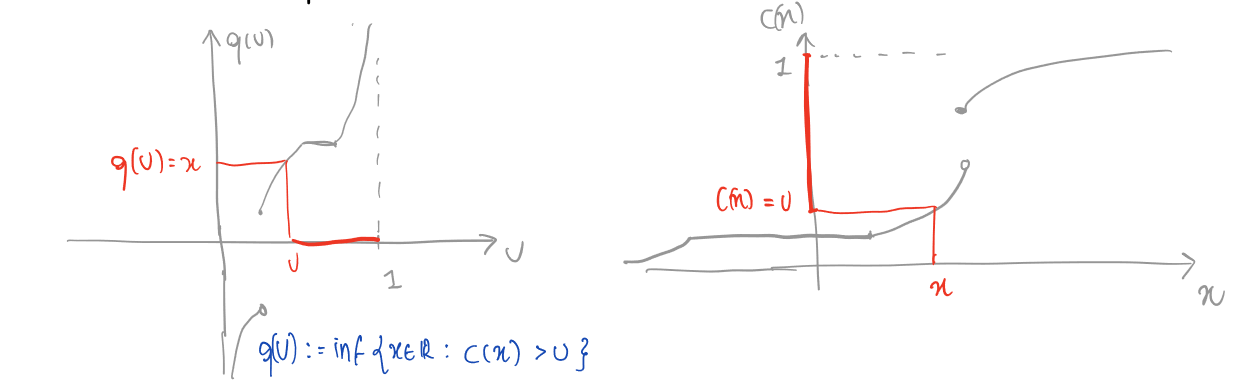
\includegraphics[width=\linewidth]{screenshot021}
		\caption[Whatever. I hate exercises]{Ok but tikz are hard and long... ;) that is WHY i use them.}
		\label{fig:screenshot021}
	\end{figure}
	\item We construct $\mu$ as in the previous two points. That $\mu$ is unique thanks to the theorem on uniqueness of measures (since $\mu$ is defined on the p-system $(-\infty,x]$). Vice versa, given the probability measure $\mu$ on $\left(\Rext,\B\left(\Rext\right)\right)$ we define
	\begin{align*}
		c:&\R\to[0,1]\\
		&x\mapsto c(x)=\mu([\infty,x]).
	\end{align*}
	We notice that $c$ is a cumulative distribution function. Indeed:
	\begin{itemize}
		\item $c$ is increasing (it is non-decreasing but whatever):
		\begin{equation*}
			\every x_1\leq x_2\qquad c(x_1)=\mu[\infty,x_1]\leq\mu[-\infty,x_2]=c(x_2)
		\end{equation*}
		since $[-\infty,x_1]\subseteq[-\infty,x_2]$.
		\item $c$ is right continuous: let $x\in\R$ be fixed and let $A_n=[-\infty,x+\frac{1}{n}],\;\every n\geq1$. Clearly $A_n\in\B(\R)$ and $A_n\searrow a:=[-\infty,x]$. Then by properties of measures we know that 
		\begin{equation*}
			\lim_{n \to \infty}\mu(A_n)=\mu(A)
		\end{equation*}
		and since $\mu(A_n)=c(x+\frac{1}{n})$ and $\mu(A)=c(x)$ we conclude
		\begin{equation*}
			\lim_{n \to \infty}c\left(x+\frac{1}{n}\right)=c(x).
		\end{equation*}
	\end{itemize}
\end{enumerate}
\begin{exercise}
	Let $X_1,X_2,\ldots,X_n\in L^{1}$. Show that $\{X_1,X_2,\ldots,X_n\}$ is uniformly integrable.
\end{exercise}
We know that a \rv{} is uniformly integrable if $\lim_{b\to\infty}\sup_{X\in K}\ev\left[|X|\indi_{\{(|X|>b)\}}\right]=0$. So, since we are operating over a finite set, we can swap $\lim$ and $\max$ to conclude that this is equivalent to showing
\begin{equation}
	\max_{i=1,\ldots,n}\lim_{b\to\infty}\ev\left[|X_i|\indi_{\{X>b\}}\right]=0\tag{$\ast$}\label{session2ex31}
\end{equation}
Let's fix $i$. We have
\begin{equation}
	\lim_{b\to\infty}\ev\left[|X_i|\indi_{\{|X_i|>b\}}\right]=\ev\ubracketthin{\left[\lim_{b\to\infty}|X_i|\indi_{\{|X_i|>b\}}\right]}_{\mathclap{\text{this is $0$ because $|X_i|\in L^{1}$. }}}=0.\tag{$\ast\ast$}\label{session2ex32}
\end{equation}
Here we can swap expectation and limit thanks to the dominated convergence theorem, since $|X_i|$ (weakly) dominates $|X_i|\indi_{\{|X_i|>b\}}$. Moreover, $\lim_{b\to\infty}|X_i|\indi_{\{|X_i|>b\}}$ is 0 because being in $L^{1}$ means having "low" tails. So \ref{session2ex32} holds for all $i$ and therefore \ref{session2ex31} holds.
\begin{exercise}
	Let $\{X_i\}$ be a family of uniformly integrable variables on $(\Omega,\F,\pr)$ and let $X\in\lone$. Show that the family $\{X_i-X\}$ is uniformly integrable.
\end{exercise}
Let $K:=\{X_i-X\}$. We use the $\varepsilon-\delta$ characterization for uniform integrability. So we should check that:
\begin{enumerate}
	\item $\sup_{Y\in K}\ev[Y]$;
	\item $\every\varepsilon\exists\delta:\text{if $F\in\F$ with $\pr(F)\leq\delta$}$ then $\sup_{Y\in K}\ev\left[|Y|\indi_F\leq\varepsilon\right]$.
\end{enumerate}
\begin{enumerate}
	\item We have
	\begin{align*}
		\sup_{Y\in K}\ev|Y|&=\sup_i\ev\left|X_i-X\right|\\
		&\leq\sup_i\left(\ev\left|X_i\right|+\ev\left|X\right|\right)\\
		&\leq\ubracketthin{\ev\left|X\right|}_{<\infty\text{ bc U.I.}}+\sup_i\ubracketthin{\ev\left|X_i\right|}_{<\infty\text{ bc $\in\lone$}}<\infty
	\end{align*}
	The third step is simple triangle inequality...
	\item Since $\{X_i\}$ is uniformly integrable, for any $\varepsilon_1$ there exists a $\delta_1$ such that if $\pr(F)<\delta_1$ then $\sup_i\ev\left[|X_{i}|\right]\leq1\varepsilon_1$. On the other hand, the fact that $X$ is in $\lone$ means that $\{X\}$ is uniformly integrable because $\lim_{b\to\infty}\ev\left[|X|\indi_{\{|X|>b\}}\right]$, so for each $\varepsilon_2$ we can find a $\delta_2$ such that if $\pr(F)\leq\delta_2$ then $\sup_i\ev\left[|X|\indi_F\right]\leq\varepsilon_2$. Then, for any $\varepsilon>0$, choose $\varepsilon_1=\varepsilon_2=\frac{\varepsilon}{2}$. We need to find our $\delta$ so we say $\delta=\min\{\delta_1,\delta_2\}$. In this way, for $F\in\F$ such that $\pr(F)\leq\delta$ (which means that is also $\leq\delta_1$ and $\leq\delta_2$) we have
	\begin{align*}
		\sup_{Y\in K}\ev\left[|Y|\indi_F\right]&=\sup_i\ev\left[|X_i+X|\indi_F\right]\\
		&\leq\sup_i\ev\left[|X_i|\indi_F\right]+\ev\left[|X|\indi_F\right]\\
		&\leq\frac{\varepsilon}{2}+\frac{\varepsilon}{2}=\varepsilon.
	\end{align*}
\end{enumerate}
\begin{exercise}
	Let $X$ and $Y$ be \rv s with values in $(\R_+,\B(\R_+))$ and $(\R,\B(\R))$ respectively. Let $Z=(X,Y)$ and 
	\begin{equation*}
		\pr_Z(\dx,\dy)=\lambda\frac{e^{-\lambda x}}{\sqrt{2\pi x}}e^{-\frac{y^{2}}{2x}}\dx\dy\qquad x\in\R_+,y\in\R
	\end{equation*}
	be the joint density function.
	\begin{enumerate}[\circnum]
		\item Find the marginal distribution $\pr_X$ of $X$.
		\item Find the transition kernel $K$ from $(\R_{+}),\B(\R_+)$ to $(\R,\B(\R))$ such that 
		\begin{equation*}
			\pr_Z=\pr_X\times K\qquad\left(\pr_Z(\dx,\dy)=\pr_X(\dx)\cdot K(x,\dy)\right).
		\end{equation*}
		Prove that $K$ is a Markov transition kernel.
		\item Find the marginal distribution $\pr_Y$ of $Y$. Hint: use that
		\begin{equation*}
			\int_0^\infty\frac{1}{\sqrt{x}}\cdot e^{-\gamma x}\cdot e^{-\frac{\beta}{x}}\dx=\sqrt{\frac{\pi}{\gamma}}\cdot e^{-2\sqrt{\beta\gamma}}\qquad\gamma>0,\beta\geq0.
		\end{equation*}
		\item Determine whether $X$ and $Y$ are independent.
	\end{enumerate}
\end{exercise}
\begin{enumerate}[\circnum]
	\item Let's find $\pr_X(A)$ for each $A\in\B(\R_+)$.
	\begin{align*}
		\pr_X(A)&=\pr_Z(A\times\R)=\int_{A\times\R}\pr_Z(\dx,\dy)\\
		&=\int_{A}\int_\R\lambda\frac{e^{-\lambda x}}{\sqrt{2\pi x}}e^{\frac{-y^{2}}{2x}}\dx\dy\\
		&=\int_A\lambda e^{-\lambda x}\ubracketthin{\int_\R\frac{1}{\sqrt{2\pi x}}e^{-\frac{y^{2}}{2x}}\dy}_{\text{density of }\mathcal{N}(0,x)}\,\dx\\
		&=\int_A\lambda e^{-\lambda x}\cdot1\cdot\dx.
	\end{align*}
	So $\pr_X(\dx)=\lambda e^{-\lambda x}\sim\mathsf{Exp}(\lambda)$.
	\item Since we can now write
	\begin{equation*}
		\pr_Z(\dx,\dy)=\pr_X(\dx)\frac{1}{\sqrt{2\pi x}}e^{-\frac{y^{2}}{2x}}\dy
	\end{equation*}
	then we see that \[K(x,\dy)=\frac{1}{\sqrt{2\pi x}}e^{-\frac{y^{2}}{2x}}\dy\]
	or, more formally, for $B\in\B(\R)$ we have
	\begin{equation*}
		K(x,B)=\int_B\frac{1}{\sqrt{2\pi x}}e^{-\frac{y^{2}}{2x}}\dy.
	\end{equation*}
	Let's now check that $K(x,B)$ is a Markov transition kernel:
	\begin{itemize}
		\item it is a transition kernel because
		\begin{enumerate}
			\item for $B\in\B(\R)$ fixed, $K(\cdot,B)$ is positive and measurable (it is even continuous);
			\item for $x\in\R_{+}$ fixed, $K(x,\cdot)$ is a measure on $\B(\R)$: in particular by inspection we see that it is a Gaussian measure with mean 0 and variance $x$.
		\end{enumerate}
		\item It is a Markov kernel because $K(x,\R)=1\,\every x$ since $K(x,\cdot)$ is a probability measure $\every x\in\R$.
	\end{itemize}
	\item Let's find $\pr_Y(B)$ for every $B\in\B(\R)$.
	\begin{align*}
		\pr_B(B)&=\pr_Z(\R_+\times B)=\int_{\R_+\times B}\lambda e^{-\lambda x}\frac{e^{\frac{y^{2}}{2x}}}{\sqrt{2\pi x}}\dx\dy\\
		&=\int_{B}\left(\int_{\R_{+}}\lambda\frac{e^{-\lambda x}}{\sqrt{2\pi x}}e^{\frac{-y^{2}}{2x}}\dx\right)\dy\\
	\end{align*}
	Now use the hint with $\gamma=\lambda,\,\beta=\frac{y^{2}}{2}$ to get
	\begin{align*}
		\frac{1}{\sqrt{2\pi}}\lambda\int_{\R_+}e^{-\lambda x}\frac{1}{\sqrt{x}}e^{\frac{y^{2}}{2x}}\dx&=\frac{\lambda}{\sqrt{2\pi}}\cdot\frac{\sqrt{\pi}}{\sqrt{\lambda}}\cdot e^{-2\sqrt{\lambda\cdot\frac{y^{2}}{2}}}\\
		&=\sqrt{\frac{\lambda}{2}}e^{-\sqrt{2\lambda}\cdot|y|}.
	\end{align*}
	So our function becomes
	\begin{equation*}
		\int_B\frac{1}{2}\sqrt{2\lambda}e^{-\sqrt{2\lambda|y|}}\dy.
	\end{equation*}
	Which is the probability density function of a two-sided exponential \rv. Thus $\pr_Y(\dy)=\frac{1}{2}\sqrt{2\lambda}e^{-\sqrt{2\lambda}|y|}\dy$.
	\item We observe that $\pr_X\cdot\pr_Y\neq \pr_Z$ so $X$ and $Y$ are not independent.
\end{enumerate}
\subsection{Exercise class 3}
\begin{exercise}
	Let $X,Y$ be independent \rv s $\sim\normale(0,1)$. Compute the joint distribution of $(X+Y,X-Y)$.
\end{exercise}
The vector is Gaussian, since it is a linear combination of Gaussian \rv s.
\begin{align*}
	W&:=(X+Y,X-Y)=(W_1,W_2)\\
	Z&:=(X,Y).
\end{align*}
We write $W$ in terms of $Z$:
\begin{equation*}
	W=\mu+\mathbf{A}Z\qquad\text{for some }\mu=(\mu_1,\mu_2)\text{ and }\mathbf{A}=\begin{bmatrix}
		a_{11}&a_{12}\\a_{21}&a_{22}
	\end{bmatrix}.
\end{equation*}
Clearly $\mu=(0,0)$ because
\begin{align*}
	\ev W_1&=\ev X+Y=\ev X+\ev Y=0\\
	\ev W_2&=\ev X-Y=\ev X-\ev Y=0
\end{align*}
So now we have
\begin{equation*}
	\begin{array}{l}
		W_1=X+Y=a_{11}X+a_{12}Y\\
		W_2=X-Y=a_{21}X+a_{22}Y
	\end{array}\implies\mathbf{A}=\begin{bmatrix}
	a_{11}&a_{12}\\a_{21}&a_{22}
	\end{bmatrix}=\begin{bmatrix}
	1&1\\1&-1
	\end{bmatrix}
\end{equation*}
Let's calculate the covariance matrix $\Gamma$ of $W$, given by
\begin{equation*}
	\Gamma=\mathbf{A}\trns{\mathbf{A}}=\begin{bmatrix}
		1&1\\1&-1
	\end{bmatrix}\begin{bmatrix}
	1&1\\1&-1
	\end{bmatrix}=\begin{bmatrix}
	2&0\\0&2
	\end{bmatrix}
\end{equation*}
Since $\mathsf{det}(\Gamma)=4\neq0$ then $\Gamma$ has full rank so the \rv{} $W$ has density given by
\begin{equation*}
	f_W(W_1,W_2)=\frac{1}{(2\pi)^{\frac{2}{2}}}\cdot\frac{1}{\sqrt{\mathsf{det}(\Gamma)}}e^{-\unmezz(\begin{smallmatrix}
			W_1&W_2
	\end{smallmatrix})\Gamma^{-1}\left(\begin{smallmatrix}
	W_1\\W_2
\end{smallmatrix}\right)}.
\end{equation*}
Compute $\Gamma^{-1}$:
\begin{equation*}
	\Gamma^{-1}=\frac{1}{\mathsf{det}(\Gamma)}\begin{bmatrix}
		2&-0\\-0&2
	\end{bmatrix}=\begin{bmatrix}
	\unmezz&0\\0&\unmezz
	\end{bmatrix}
\end{equation*}
And now plug the results inside the density formula:
\begin{align*}
	f_W(W_1,W_2)&=\frac{1}{(2\pi)^{\frac{2}{2}}}\cdot\frac{1}{\sqrt{\mathsf{det}(\Gamma)}}e^{-\unmezz(\begin{smallmatrix}
			W_1&W_2
		\end{smallmatrix})\Gamma^{-1}\left(\begin{smallmatrix}
			W_1\\W_2\end{smallmatrix}\right)}\\
		&=\frac{1}{(2\pi)^{\frac{2}{2}}}\cdot\frac{1}{2}e^{-\unmezz(\begin{smallmatrix}
				W_1&W_2
			\end{smallmatrix})\left(\begin{smallmatrix}
			\unmezz&0\\0&\unmezz
			\end{smallmatrix}\right)\left(\begin{smallmatrix}
				W_1\\W_2\end{smallmatrix}\right)}\\
			&=\frac{1}{4\pi}e^{-\unmezz(\unmezz W^{2}_{1}+\unmezz W^{2}_{2})}.
\end{align*}
So this is the density of the \rv{} $W=(X+Y,X-Y)$.
\begin{remark}
	Since $\Gamma_{12}=\Gamma_{21}=0$ we have $W_1\independent W_2$. We can see this also because the joint distribution factorizes in the product of the marginal distributions.
		\begin{equation*}
		f_W(W_1,W_2)=\underbrace{\frac{1}{\sqrt{2\pi\cdot 2}}e^{-\frac{1}{4}W^{2}_1}}_{\sim\normale(0,2)}\cdot\underbrace{\frac{1}{\sqrt{2\pi\cdot 2}}e^{-\frac{1}{4}W^{2}_2}}_{\sim\normale(0,2)}
		\end{equation*}
\end{remark}
\begin{exercise}
	Let $X,Y$ be independent real \rv s with distributions $\mu_{X}$ and $\mu_{Y}$ respectively. Show that the distribution of $Z:=X+Y$ denoted $\mu_{Z}$ is given by 
	\begin{equation*}
		\mu_Z(B)=\int_\R\mu_{X}(B-x)\mu_Y(\dx)\qquad\every B\in\B(\R)
	\end{equation*}
	where
	\begin{equation*}
		\{B-x\}:=\{y-x\in\R\text{ s.t. }y\in B\}.
	\end{equation*}
	Note that since $X+Y=Y+X$ we also have 
	\begin{equation*}
		\mu_Z(B)=\int_\R\mu_Y(B-x)\mu_X(\dx)
	\end{equation*}
\end{exercise}
Take $B\in\B(\R)$. We have
\begin{align*}
	\mu_Z(B)&=\pr(Z\in B)\\
	&=\pr(X+Y\in B)\\
	&=\ev\left[\indi_{\{X+Y\in B\}}\right].
\end{align*}
We know that $\mu_{(X,Y)}=\mu_X\cdot\mu_Y$ since $X\independent Y$, so whe have that
\begin{align*}
		\mu_Z(B) &=\pr(X+Y\in B)\\
		&=\ev\left[\indi_{\{X+Y\in B\}}\right]\\
				&=\int_\R\int_\R\indi_{\{X+Y\in B\}}\mu_{(X,Y)}(\dx,\dy)\\
	 &=\int_\R\int_\R\indi_{\{X+Y\in B\}}\mu_X(\dx)\mu_Y(\dy)\\
	 &=\int_\R\int_\R\indi_{B}(x+y)\mu_X(\dx)\mu_{Y}(\dy).\tag{$\ast$}\label{funziona}
\end{align*}
Now consider
\begin{equation*}
	\indi_{B}(x+y)=\indi_{\{B-x\}}(y)=\begin{cases}
		1 &\text{ if }x+y\in B\iff y\in\{B-x\}\\
		0 &\text{ if }x+y\notin B\iff y\notin\{B-x\}
	\end{cases}.
\end{equation*}
Now consider \ref{funziona}:
\begin{align*}
	\int_\R\int_\R\indi_{B}(x+y)\mu_X(\dx)\mu_{Y}(\dy)&=\int_\R\int_\R\indi_{\{B-x\}}(y)\mu_{X}(\dx)\mu_Y(\dy)\\
	&=\int_\R\Biggl(\ubracketthin{\int_\R\indi_{\{B-x\}}(y)\mu_{Y}(\dy)}_{\mathclap{\int_{\{B-x\}}\mu_{Y}(\dy)=\mu_Y(B-x)}}\Biggr)\mu_{X}(\dx)\\
	&=\int_\R\mu_{Y}(B-x)\mu_{X}(\dx)
\end{align*}\begin{exercise}
Let $X,Y$ be independent \rv s with densities $f_X,f_Y$. Show that $Z:=X+Y$ also has a density function given by
\begin{equation*}
	f_Z(z):=\int_\R f_{X}(x)f_Y(z-x)\dx,\qquad z\in\R.
\end{equation*}
\end{exercise}
Take $B\in\B(\R)$. The law of $Z$, $\mu_Z$, is such that
\begin{equation*}
	\mu_Z(B)=\pr(Z\in B)
\end{equation*}
and we want to show that indeed
\begin{equation*}
	\pr(Z\in B)=\int_{B}f_Z(z)\dz.
\end{equation*}
Using what we found in exercise 2 we have that
\begin{align*}
	\mu_Z(B)&=\int_\R\mu_Y(B-x)\mu_X(\dx)\\
	&=\int_\R\int_{B-x}f_Y(y)\dy f_X(x)\dx.
\end{align*}
If $y\in\{B-x\}$ it means that $y=t-x$ for some $t\in B$. So we can make a change of variable $y=t-x$:
\begin{equation*}
	\int_{\{B-x\}}f_Y(y)\dy=\int_{B}f_Y(t-x)\dt
\end{equation*}
which implies
\begin{align*}
	\mu_Z(B)&=\int_\R\int_B f_Y(y)(t-x)\dt f_X(x)\dx\\
	&=\int_B\left(\int_\R f_Y(t-x)f_X(x)\dx\right)\dt\\
	&=\int_B f_Z(t)\dt.
\end{align*}
\begin{exercise}
	Let $(X_n)$ be a sequence of independent \rv s. Show that if $\lim_{n\to\infty}X_n=X\;\pr\as$ then $X=c\;\pr\as$ for some $c\in\R$.
\end{exercise}
Start from this set:
\begin{align*}
	A&=\left\{\omega:\lim_{n}X_{n}(\omega)\text{ exists}\right\}\\
	&=\left\{\omega:\liminf_{n}X_n(\omega)=\limsup_{n}X_n(\omega)\right\}.
\end{align*}
We know that $\pr(A)=1$ because we know that $X_n$ always converges and we want to show that $A\in\tau$ because this (together with independence) would allow us to apply Kolmogorov's 0-1 law's corollary that tells us that if an event is part of a tail \sa{} then it is a constant\footnote{If you have already read the theory then you know how this thing caused me a mental breakdown.}. Let's show that $\limsup_n X_n$ is $\tau$-measurable.
\begin{align*}
	\limsup_nX_n&=\inf_n\ubracketthin{\sup_{m\geq n}X_m}_{\mathclap{\text{is measurable with respect to }\bigvee_{m\geq n}\sigma(X_m)=\tau_n}}
\end{align*}
Thus $\inf_n\sup_{m\geq n}X_m$ is measurable with respect to 
\begin{equation*}
	\bigcap_{n\geq1}\bigvee_{m\geq n}\sigma(X_m)=\bigcap_{n\geq1}\tau_n=\tau
\end{equation*} 
so $\limsup_nX_n$ is $\tau$-measurable. Similarly for $\liminf$ we get that is is $\tau$-measurable so $A\in\tau$. \\
We recall that $X$ is such that
\begin{equation*}
	X(\omega)=\lim_{n\to\infty}X_{n}(\omega)\qquad\every\omega\in A\in\tau.
\end{equation*}
Introduce
\begin{equation*}
	Y(\omega)=\begin{cases}
		X(\omega)&\text{if }\omega\in A\\
		0&\text{if }\omega\notin A.\\
	\end{cases}
\end{equation*}
We introduced this new \rv{} because we are technically working with the \textit{limit} of $X_n$ (which is a sequence) and measurability of limits is not a beautiful thing to handle.
By definition $X=Y$ $\pr-\as$ (because $\pr(A^{c})=0$) and $Y$ is $\tau$-measurable because $A\in\tau$. This implies that $X$ is $\tau$-measurable. By corollary of the Kolmogorov's 0-1 law, $X=c$ $\pr-\as$ for some $c\in\R$.
\begin{exercise}
	Let $(X_n)$ be a sequence of i.i.d. \rv s with $X_n\sim\mathsf{Exp}(1)$ with density
	\begin{equation*}
		f(x)=\begin{cases}
			e^{-x}&\text{if }x\geq 0\\
			0&\text{else.}
		\end{cases}
	\end{equation*}
	Determine whether
	\begin{equation*}
		\frac{1}{n}\max\left\{X_1,X_2,\ldots,X_n\right\}\convas0.
	\end{equation*}
\end{exercise}
We guess yes because why not. Let $\varepsilon>0$. Take the set
\begin{equation*}
	B_n:=\left\{\omega:X_n(\omega)\geq n\varepsilon\right\}.
\end{equation*}
This gives us
\begin{align*}
	\pr(B_n)&=\ev\left[\indi_{B_{n}}\right]\\
	&=\int_{n\varepsilon}^{+\infty}e^{-x}\dx=e^{-n\varepsilon}.
\end{align*}
Thus $\sum_{n}\pr(B_{n})=\sum_{n}e^{-n\varepsilon}<\infty$. By Borel-Cantelli 1 we have 
\begin{equation*}
	\pr\left(\left\{B_{n}\;\io\right\}\right)=0.
\end{equation*}
Take the complement:
\begin{equation*}
	\pr(\{B^{c}_{n}\;\text{f.o.}\})=1.
\end{equation*}
For every $\omega\in\left\{B_n^c\;\text{f.o.}\right\}$ there exists $m(\omega,\varepsilon)$ such that $\every n>m(\omega,\varepsilon)$ then $\ubracketthin{X_n(\omega)<n\varepsilon}_{B_n^c}$.
Set 
\begin{equation*}
	M(\omega,\varepsilon):=\max\left\{X_1(\omega),X_2(\omega),\ldots,X_{m(\omega,\varepsilon)}(\omega)\right\}
\end{equation*}
so that for $\every n$ we have
\begin{equation*}
	\max\{X_1(\omega),X_2(\omega),\ldots,X_n(\omega)\}\leq M+n\varepsilon
\end{equation*}
so
\begin{equation*}
	\frac{1}{n}\max\{X_1(\omega),X_2(\omega),\ubracketthin{\ldots}_{\mathclap{X_m(\omega),X_{m+1}(\omega),\ldots}},X_n(\omega)\}\leq\frac{M(\omega,\varepsilon)}{n}+\varepsilon.
\end{equation*}
Check the limit:
\begin{align*}
	\limsup_{n}\frac{1}{n}\max\{X_1(\omega),\ldots,X_n(\omega)\}&\leq \limsup_{n}\frac{M(\omega,\varepsilon)}{n}+\varepsilon\\
	&=\lim_{n}\frac{M(\omega,\varepsilon)}{n}+\varepsilon=\varepsilon.
\end{align*}
Now we take the limit as $\varepsilon\to0$:
\begin{equation*}
	\limsup_{n}\frac{1}{n}\max\{X_1(\omega),\ldots,X_n(\omega)\}\leq\lim_{e\to0}\varepsilon=0
\end{equation*}
Thus, using the fact that $X_i$ are positive, we conclude
\begin{equation*}
	\lim_{n\to\infty}\frac{1}{n}\max\{X_1(\omega),\ldots,X_n(\omega)\}=0.
\end{equation*}
Since this holds for $\every \omega\in\{B_{n}^x\text{ ev.}\}$ and $\pr(\{B^c_n\text{ ev.}\})=1$ we have
\begin{equation*}
	\frac{1}{n}\max\{X_1,\ldots,X_n\}\to0\qquad \as{}
\end{equation*}
\begin{exercise}
	Let $(X_i)$ be independent \rv s non negative such that
	\begin{equation*}
		\pr(X_i\geq\delta)\geq\varepsilon,\qquad\every i
	\end{equation*}
	for some fixed $\delta,\varepsilon>0$. Determine whether $S_n=\sum_{i=1}^{n}X_i$ converges a.s. as $n\to\infty$.
\end{exercise}
Guess: $S_n$ diverges to $+\infty$ because the \rv s $X_i$ are such that $\{X_i>\delta\}$ has positive probability. We claim
\begin{equation}
	\limsup_n\{X_i\geq\delta\}\subset\{\lim_{n\to\infty}S_n=\infty\}\tag{\FiveFlowerOpen}\label{proviamoilfiore}
\end{equation}
Let's prove it.
\begin{align*}
	\omega\in\limsup_{i}\{X_i\geq\delta\}&=\bigcap_{i\geq1}\bigcup_{m\geq i}\{X_m\geq\delta\}\\
	&=\{X_i\geq\delta\;\io\}.
\end{align*}
This means that $\exists$ a subsequence $i_{k}$ such that $X_{i_{k}}(\omega)\geq\delta$. Summing over $k$ we get
\begin{equation*}
	\sum_{k=1}^{\infty}X_{i_{k}}(\omega)\geq\sum_{k=1}^{\infty}X_{i}(\omega)=\infty.
\end{equation*}
So taking the limit we obtain
\begin{align*}
	\lim_{n\to\infty}S_n^{(\omega)}&=\lim_{n\to\infty}\sum_{i=1}^{n}X_i(\omega)\\
	&=\sum_{i=1}^{\infty}X_i(\omega)\\
	&\geq\sum_{k=1}^\infty X_{i_{k}}(\omega)=\infty\implies\lim_{n \to \infty}S_n(\omega)=\infty
\end{align*}
hence \ref{proviamoilfiore}\footnote{Yes, I have ONLY NOW discovered dingbats. My future endeavours will have more of them, do not worry. Even if they look like shit with this font, on god.} holds. We now apply Borel-Cantelli 2.
\begin{revise}
	\begin{proposition}
		\emph{``\textit{Divergence}''}. Let ${(A_{n})}_{n}$ be a sequence of pairwise independent events. 
		\begin{equation*}
			\text{If }\sum_{n=1}^{\infty}\pr(A_n)=+\infty\text{ then }\ubracketthin{\sum_{n=1}^{\infty}\indi_{A_{n}}}_{\mathclap{=\pr(\{A_n\,\io\})}}=\infty\;\as{}
		\end{equation*}
	\end{proposition}
	An equivalent formulation of Borel-Cantelli 2 is:
	\begin{proposition}
		Take a sequence of Bernoulli \rv s $B_{n}$ defined as
		\begin{equation*}
			B_n=\begin{cases}
				1&\text{on }A_n\\
				0&\text{on }A_n^c\\
			\end{cases}\qquad(\text{or, more simply, }B_n=\indi_{A_{n}})
		\end{equation*}
		so that $B_n$ is a Bernoulli \rv{} and we have 
		\begin{equation*}
			\ev B_{n}=\pr(A_{n}).
		\end{equation*}
		The $B_n$ are pairwise independent.
		\begin{equation*}
			\text{If }\sum_{n=1}^{\infty}\ev B_{n}=\infty\text{ then }\sum_{n=1}^{\infty}B_n=\infty\;\as{}
		\end{equation*}
	\end{proposition}
	Remember that $\limsup_n\{X_n=1\}$ is the same as saying that $\{X_n=1\;\io\}$.
\end{revise}
In our case we have $B_i=\{X_i\geq\delta\}$. We know that $\pr(B_i)\geq\epsilon$ by assumption, so
\begin{equation*}
	\sum_{i=1}^\infty \pr(B_i)=\infty.
\end{equation*}
Moreover, the $B_i$ are independent. Hence we can apply BC-2 and say that
\begin{equation*}
	\pr(\{X_i\geq\delta\}\,\io)=1\iff\pr(\limsup_{i}\{X_i\geq\delta\})=1.
\end{equation*}
By \ref{proviamoilfiore} we have
\begin{equation*}
	1=\pr(\limsup\{X_i\geq\delta\})\leq\pr(\lim_{n}S_n=\infty)
\end{equation*}
hence 
\begin{equation*}
	\pr(\lim_n S_n=\infty)=1
\end{equation*}
which means that we have almost sure divergence of the sum.
\subsection{Exercise class 4}
\begin{revise}
	Hi bitch. Remember all the types of convergence? Me neither!
		\begin{enumerate}[\HandRight]
			\item \emph{Convergence in $\lp$}:
			\begin{equation*}
				X_n\convlp X
			\end{equation*}
			if $X_n,X\in\lp$ and $$\ev|X_n-X|^{p}\to0 \text{ as }  n\to\infty.$$\\
			A necessary (but not sufficient...) condition for convergence in $\lp$ is that 
			 \begin{equation*}
				\ev|X_n|^{p}\to\ev|X|^{p}.
			\end{equation*}
			\item \emph{Convergence in probability}:
			\begin{equation*}
				X_n\convpr X
			\end{equation*}
			if $\every\varepsilon>0$ we have \\
			\begin{equation*}
				\pr(|X_n-X|>\varepsilon)\to0\qquad\text{as }n\to\infty.
			\end{equation*}
			\item \emph{Almost sure convergence}:
			\begin{equation*}
				X_n\convas X
			\end{equation*}
			if $\exists\Omega'\subset\Omega$ with $\pr(\Omega')=1$ such that
			\begin{equation*}
				X_n(\omega)\to X(\omega)\qquad\every\omega\in\Omega'.
			\end{equation*}
			\item \emph{Convergence in distribution}:
			\begin{equation*}
				X_n\convd X
			\end{equation*}
			if $F_n(x)\to F(x)$ for any point $x$ such that $F(x)$ is continuous. Here $F_n$ and $F$ denote the cumulative distribution functions of $X_n$ and $X$.
			\item[\PencilRightDown] \emph{Link between different convergence modes}:
			\begin{equation*}
				\begin{array}{ccccc}
					X_{n}\convlp X&\implies&X_n\convpr X&\impliedby&X_n\convas X\\
					&&\Downarrow&&\\
					&&X_n\convd X.&&
				\end{array}
			\end{equation*}
			\item[\PencilRightDown]\emph{Properties:}
			\begin{enumerate}[\ArrowBoldRightStrobe]
				\item if $X_n\convpr X$ and $X_n\convpr Y$ then $X=Y$ \as{};
				\item if $X_n\convlp X$ and $\lim_n X_n$ exists \as, then $X_n\convas X$.
			\end{enumerate}
		\end{enumerate}
\end{revise}
\begin{exercise}
	Let $X_n$ be a sequence of independent \rv s with $X_n\sim\mathsf{Be}(\frac{1}{n})$. Determine whether $X_n$ converges \as{} or in $\lp$ for some $p\geq1$. 
\end{exercise}
I will now stop\footnote{This is a lie.} with the stupid \LaTeX{}  symbols.
\begin{enumerate}[\faPaperPlane]
	\item $\lp$ convergence: note that 
	$$\ev|X_n|^{p}=\ev X_n^{p}=1^{p}\cdot\frac{1}{n}
	+0^{p}\cdot(1-\frac{1}{n})
	=\frac{1}{n}\xrightarrow[]{n\to\infty}=0,\qquad\every p>0.$$
	Hence the candidate limit is $X=0$. Let's check
	\begin{equation*}
		\ev|X_n-0|^{p}=\ev|X_n|^{p}=\frac{1}{n}\to0
	\end{equation*}
	so \begin{equation*}
		X_n\convlp X,\qquad\every p\geq1.
	\end{equation*}
	\item Almost sure convergence: we note that 
	\begin{equation*}
		\sum_{n=1}^{\infty}\pr(X_n=1)=\sum_{n=1}^{\infty}\frac{1}{n}=+\infty
	\end{equation*}
	hence by BC-2 we have that
	\begin{equation*}
		\pr(\limsup_n\{X_n=1\})=1.
	\end{equation*}
	This implies that we cannot have $X_n\convas 0$.
\end{enumerate}
\begin{exercise}
	Let ${(X_{n})}_{n}$ be a sequence of i.i.d. \rv s with $X_{n}\sim\mathsf{U}(0,1)$.  Let $Y_{n}=\min\{X_1,X_2,\ldots,X_n\}$. Determine whether $Y_n$ converges a.s. and in $\lp$ for some $p\geq1$.
\end{exercise}
We must figure out the distribution of $Y_n$. for $x\in(0,1)$ we have:
\begin{align*}
	\pr(Y_n>x)&=\pr(X_1>x,X_2>x,\ldots,X_n>x)\\
	&=\pr(X_1>x)\cdot\pr(X_2>x),\cdot\ldots\cdot\pr(X_n>x)\\
	&=(1-x)^{n}.
\end{align*}
Therefore,
\begin{equation*}
	\pr(Y_n\leq x)=1-(1-x)^{n}=\int_{0}^{x}f_{Y_{n}}(x)\dy
\end{equation*}
so taking the derivative we have:
\begin{equation*}
	f_{Y_{n}}(y)=\begin{cases}
		n(1-y)^{n-1}&\text{for }y\in(0,1)\\
		0&\text{else.}
	\end{cases}
\end{equation*}
Let's check if $\ev|Y_n|^{p}$ converges for some $p$. We start with $p=1$.
\begin{revise}
	Remember integration by parts? Lmao.
	$$\int fg'=fg-\int f'g$$
\end{revise}
\begin{align*}
	\ev|Y_{n}|&=\ev Y_{n}\\
	&=\int_0^1\ubracketthin{y}_{\mathclap{f}}\ubracketthin{n(1-y)^{n-1}}_{g'}\dy\\
	&=y\left(-(1-y)^{n}\right)\Big|^1_0-\int_0^1-(1-y)^{n}\dy\\
	&=0+-\frac{(1-y)^{n+1}}{n+1}\Big|^1_0\\
	&=0+\frac{1}{1+n}
\end{align*}
Hence $\ev|Y_n|\xrightarrow[n\to\infty]{}0$, so the candidate $Y$ such that $\ev|Y_n-Y|\to0$ is 0. This implies $\ev|Y_n-0|=\ev|Y_n|\to0$ so that we have $Y_n\xrightarrow{\lone}0$. What about convergence in $\lp$ though? First check a.s. convergence. \\
By definition of $Y_n$ we have $Y_{n+1}(\omega)\leq Y_n(\omega)$ for almost all $\omega$; this means that $Y_n$ is monotone $\pr$-almost surely. This implies that $Y_n$ has a limit $\pr$-almost surely, say $Y$ (moreover, $Y_n(\omega)\geq0$ hence $Y(\omega)\geq0$ $\pr$-a.s.). \\
By uniqueness of the limit\footnote{$Y_n\xrightarrow{\lone}0\implies Y_n\convpr0$; $Y_b\convas Y\implies Y=0\;\pr-\as$} we have that $Y=0$. Hence we conclude $Y_n\convas 0$.\\
To check for convergence in $\lp$, if we can apply the dominated convergence theorem then we have: 
\begin{equation*}
	\lim_{n\to\infty}\ev|Y_n-Y|^{p}=\ev\left[\lim_{n\to\infty}|Y_n|^{p}\right]=0.
\end{equation*}
Here dominated convergence works because $0\leq X_{k}\leq 1$ hence $|Y_n|\leq1$ and $|Y_n|^{p}\leq1$ where 1 is integrable. Moreover, the a.s. limit $Y=0$ is also integrable.
\begin{exercise}
Let $(\Omega,\F,\pr)=\left([0,1],\B([0,1]),\leb_{(0,1)}\right)$. Let $$X_n(\omega)=n\indi_{\left[0,\frac{1}{n}\right]}(\omega).$$
Determine whether $X_n$ converges a.s. or in $L^{p}$ for some $p\geq1$.
\end{exercise}
Let's calculate $\ev|X_n|^{p}$ for some $p\geq 1$.
\begin{equation*}
	\ev|X_n|^{p}=n^{p}\cdot\pr\left(\left[0,\frac{1}{n}\right]\right)+0^{p}\cdot\pr\left(\left[\frac{1}{n},1\right]\right)=n^{p}\cdot\frac{1}{n}=n^{p-1}
\end{equation*}
which diverges for $n\to\infty$ if $p>1$. Thus there can be no $\lp-convergence$ for $p>1$.\\
Let's check a.s. convergence. For any $\omega>0\;\exists N=N(\omega)\text{ s.t. }\every n>N$ then $X_n(\omega)=0$ (since the interval $\left[0,\frac{1}{n}\right]$ shrinks). Hence $X_n(\omega)\to0\;\every\omega\;\pr-\as$ given that $\pr([0,1])=1$. \\
\faExclamationTriangle\, It does not converge for $\omega=0$ but $\{\omega=0\}$ has Lebesgue measure zero.\\
Back to $\lp$-convergence with $p=1$: if $p=1$ then $\ev|X_n|=1$ but by uniqueness of the limit we should have $X=0$ and $\ev|X|=0\neq 1$ so we do not have convergence in $\lone$.
\begin{exercise}
	Let ${(X_{n})}_{n}$ be a sequence of independent \rv s such that
	\begin{equation*}
		X_n=\begin{cases}
			0&\text{with probability }1-\frac{1}{n^2}\\
			n^{2}&\text{with probability }\frac{1}{n^{2}}.
		\end{cases}
	\end{equation*}
	Determine whether $X_n$ converges in $L^{p}$ or almost surely.
\end{exercise}
\begin{equation*}
	\ev|X_n|=\ev|X_n|=n^{2}\cdot\frac{1}{n^{2}}+0=1.
\end{equation*}
Let us check whether $X_n\convlp1$.
\begin{align*}
	\ev|X_{n}-1|&=|n^{2}-1|\frac{1}{n^{2}}+|0-1|\left(1-\frac{1}{n^{2}}\right)\\
	&=\left|\frac{n^{2}-1}{n^{2}}\right|+\left|\frac{n^{2}-1}{n^{2}}\right|\\
	&=2\left|\frac{n^{2}-1}{n^{2}}\right|\to2\neq0
\end{align*}
so there is no $\lone$ convergence. Since $\lp\implies\lone\;p\geq1$ there is no $\lp$ convergence either. What about $\as$ convergence?\\
We cannot argue directly as in Exercise 3, but do so through Borel-Cantelli: we know that $\every\varepsilon>0,\pr(|X_{n}|\geq\varepsilon)=\frac{1}{n^{2}}$, hence
\begin{equation*}
	\sum_{n=1}^{\infty}\pr\left(|X_{n}|\geq\varepsilon\right)=\sum_{n=1}^{\infty}\frac{1}{n^{2}}<\infty.
\end{equation*}
Thus by Borel-Cantelli 1 we have
\begin{equation*}
	\pr\left(\limsup_{n}\{|X_{n}|\geq\varepsilon\}\right)=0
\end{equation*}
and, taking the complement,
\begin{equation*}
	\pr\left(\liminf_{n}\{|X_{n}|<\varepsilon\}\right)=1.
\end{equation*}
Thus, $\every\varepsilon>0\;\exists\,N=N(\varepsilon)$ such that $|X_{n}(\omega)|<\varepsilon$ for $\pr$-almost all $\omega$ and this implies $X_n\convas 0$.
\begin{exercise}
	Let ${(X_{n})}_{n}$ be a sequence of independent \rv s with $X_n\sim\mathsf{Exp}(\frac{1}{n})$. Determine if $Y_{n}=\min\{X_{1},\ldots,X_{n}\}$ converges in probability.
\end{exercise}
\begin{revise}
	The exponential distribution has the following cumulative distribution function:
	\begin{equation*}
		\pr(X_{n}\geq x)=\int_0^x\frac{1}{k}e^{-\frac{\lambda}{k}}\dz=-e^{-\frac{\lambda}{k}}\Big|^{x}_{0}=1-e^{-\frac{x}{k}}
	\end{equation*}
\end{revise} 
Let's figure out the distribution of $Y_n$. We have 
\begin{align*}
	\pr(Y_{n}>y)&=\pr(X_1>y,X_2>y,\ldots,X_n>y)\\
	&=\prod_{i=1}^{n}\pr(X_i>y)\\
	&=\prod_{i=1}^{n}e^{-\frac{y}{i}}\\
	&=e^{-y\cdot\sum_{i=1}^{n}\frac{1}{i}}
\end{align*}
hence
\begin{equation*}
	Y_{n}\sim\mathsf{Exp}\left(\sumin\frac{1}{i}\right).
\end{equation*}
At the limit we would have $f_{Y}(y)=\infty\cdot e^{-\infty\cdot y}$ but we guess that $e^{-\infty}$ is stronger than $\infty$ and the limit is zero.\\
Thus we have, for $\every \varepsilon>0$,
\begin{equation*}
	\lim_{n\to\infty}\pr(|Y_{n}-0|>\varepsilon)=\lim_{n\to\infty}e^{\varepsilon\cdot\sumin\frac{1}{i}}=0
\end{equation*}
So by definition $Y_{n}\convpr0$.
\begin{exercise}
	Let ${(X_{n})}_{n}$ be a sequence of i.i.d. 
\rv s with $X_n\distexp{\lambda}$. Let
\begin{equation*}
	Y_{n}=\begin{cases}
		\frac{1}{n}&\text{if }X_n<\log n\\
		1&\text{else}.
	\end{cases}
\end{equation*}
Determine, for varying $\lambda$s, the convergence a.s., in probability or in $\lp$ for some $p\geq1$.
\end{exercise}
First, we calculate the distribution of $Y_n$:
\begin{equation*}
	\pr(Y_n\geq y)=\begin{cases}1&\text{if }Y\geq1\\\pr(X_n<\log n)&\text{if }\frac{1}{n}\leq y<1\\0&\text{if }y<\frac{1}{n}\end{cases}
\end{equation*}
where 
\begin{equation*}
	\pr(X_n<\log n)=1-e^{\lambda\cdot\log n}=1-e^{\log(n^{-\lambda})}=1-n^{-\lambda}.
\end{equation*}
From this, it looks like $pr(Y_{n}\leq y)\to1$ as $n\to\infty$. The complement of the cumulative distribution function, which we are interested in to compute the limit, is 
\begin{align*}
	\pr(Y_{n}>y)&=1-\pr(Y_{n}\leq y)\\
	&=\begin{cases}0&\text{if }Y\geq1\\n^{-\lambda}&\text{if }\frac{1}{n}\leq y<1\\1&\text{if }y<\frac{1}{n}\end{cases}
\end{align*}
and it looks like Figure \ref{backwaaaaardseverythingsbackwaaaards}.
\begin{itemize}
	\item Convergence in $\pr$: we have that $\every\varepsilon>0$ (since $Y_n\geq0$),
	\begin{equation*}
		\lim_{n\to\infty}\pr(|Y_{n}-0|>\varepsilon)=\lim_{n\to\infty}\pr(Y_{n}>\varepsilon)=0
	\end{equation*}
	which implies
	\begin{equation*}
		Y_n\convpr0,\qquad\every\lambda>0.
	\end{equation*}
	\begin{figure}[h]
		\centering
		\begin{tikzpicture}
			\begin{axis}[
				xmin=-0.5,
				ymin=0,
				xmax=6,
				ymax=3.5,
				unit vector ratio*={0 0 0},
				axis x line=bottom,
				axis y line=center,
				xtick={0,2,5},
				ytick={1.5,3},
				xticklabels={0,$\frac{1}{n}$,1},
				yticklabels={$n^{\lambda}$,1}]
				\draw[thick,red] (-0.5,3)--(2,3);
				\draw[thick,red] (2,1.5)--(5,1.5);
				\draw[thick,red] (5,0)--(6,0);
				\node[fill, red,inner sep=1pt,circle] at(2,1.5) {};
				\node[fill, red,inner sep=1pt,circle] at(5,0) {};
			\end{axis}
		\end{tikzpicture}
		\caption{It's really just like a cumulative distribution ``backwards''...}
		\label{backwaaaaardseverythingsbackwaaaards}
	\end{figure}
	\item Almost sure convergence:
We now tackle almost sure convergence and we try to apply Borel-Cantelli. Let $\varepsilon<1$ and consider
\begin{equation*}
	\sumiinf\pr(Y_{n}>\varepsilon)=\sum_{n=1}^{N^\star}1+\sum_{\mathclap{n=N^{\star}+1}}^{\infty}n^{-\lambda}\leq N^{\star}+\sumiinf n^{-\lambda}<\infty\qquad\text{if }\lambda>1
\end{equation*}
where $N^{\star}=\max\left\{n:\varepsilon<\frac{1}{n}\right\}$. Thus, by BC1 (given that $\lambda>1$),
\begin{equation*}
	\pr\left(\limsup_k\{|Y_{n}>\varepsilon\}\right)=0\iff\pr\left(\limsup_k\{|Y_{n}\leq\varepsilon\}\right)=1
\end{equation*}
i.e., $\every\varepsilon$ $\exists N=N(\varepsilon)$ such that $|Y_{n}(\omega)|\leq\varepsilon$ $\pr$-almost all $\omega$. This means that 
\begin{equation*}
	Y_{n}\convas0\qquad\qquad\text{if }\lambda>1.
\end{equation*}
On the other hand, if $\lambda\leq1$ we instead have
\begin{equation*}
	\sum_{n=1}^{\infty}\pr(Y_{n}>\varepsilon)=\sum_{n=1}^{N^\star}1+\sum_{\mathclap{n=N^{\star}+1}}^{\infty}n^{-\lambda}\leq N^{\star}+\sumiinf n^{-\lambda}=\infty\qquad\text{if }\lambda\leq1.
\end{equation*}
Thus, by BC2, we get (since $X_n\independent\implies Y_{n}\independent$)
\begin{equation*}
	\pr\left(\limsup_n\{Y_n>\varepsilon\}\right)=1
\end{equation*}
So the sequence $Y_n$ cannot converge almost surely to 0. By uniqueness f the limit, this implies that $Y_{n}\not\!\convas Y$ to any $Y$.
\item Convergence in $\lp$: let's check the necessary condition
\begin{equation*}
	\ev|Y_n|^{p}\to\ev|Y|^{p}=0.
\end{equation*}
Again, by uniqueness of the limit, we must have $Y=0$ $\pr$-a.s. Considering that $X_n\distexp{\lambda}$, we have
\begin{align*}
	\ev|Y_{n}|^{p}&=\ev Y_{n}^{p}\\
	&=\frac{1}{n^{p}}\pr(X_{n}<\log n)+1\cdot\pr(X_{n}\geq\log n)\\
	&=\frac{1}{n^{p}}\left(1-e^{\lambda\log n}\right)+e^{-\lambda\log n}\\
	&=\frac{1}{n^{p}}\left(1-n^{-\lambda}\right)+n^{-\lambda}\to0\qquad\text{ as }n\to\infty,\;\every\lambda,\;\every\lambda>0.
\end{align*}
Hence,
\begin{equation*}
	\ev|Y_{n}-0|^{p}=\ev|Y_{n}|^{p}\to0
\end{equation*}
that is 
\begin{equation*}
	Y_{n}\convlp0\qquad\every p\geq1,\;\every\lambda>0.
\end{equation*}
\end{itemize}
\subsection{Exercise class 5}	
\begin{revise}
	\begin{enumerate}[\NibSolidRight]
		\item \emph{Strong Law Of Large Numbers (SLLN)}: if $X_{n}$ are pairwise independent and identically distributed as $X$. If $\ev X$ exists ($\pm\infty$ is allowed) then
		\begin{equation*}
			\overline{X}_{n}\convas\mu.
		\end{equation*}
		\item \emph{Weak Law Of Large Numbers (WLLN)}: \begin{enumerate}
			\item if $X_{n}$ are pairwise independent and identically distributed as $X$ with $\ev X=\mu<\infty$ and $\var X=\sigma^{2}<\infty$ then 
			\begin{equation*}
				\overline{X}_{n}\to\mu\qquad\text{ in $L^{2}$, in $\pr$ and a.s.}
			\end{equation*}
			\item If $X_{n}$ are uncorrelated and $\sum_n\var\left(\frac{X_{n}}{b_{n}}\right)<\infty$ for some $(b_{n})$ strictly positive and increasing to $\infty$ then
			\begin{equation*}
				\frac{\sumin X_{i}-\ev\left(\sumin X_{i}\right)}{b_{n}}\to0\qquad\text{ in $L^{2}$ and in $\pr$.}
			\end{equation*}
			If the \rv s are independent, the convergence holds almost surely.
		\end{enumerate}
		\item \emph{Central Limit Theorem (CLT)} (easy version, whatever this may mean): if $X_{n}$ are i.i.d. \rv s with $\ev X_{i}=\mu<\infty$, $\var X=\sigma^{2}<\infty$ then
		\begin{equation*}
			\frac{\overline{X}_{n}-\mu}{\sigma/\sqrt{n}}\convd\mathsf{N}(0,1).
		\end{equation*}
		\item \emph{Weak Convergence} (for probability measures): a sequence ${(\mu_{n})}_{n}$ of probability measures converges weakly to $\mu$ if for any $f$ bounded and continuous function we have
		\begin{equation*}
			\int f\dmu_{n}\to\int f\dmu.
		\end{equation*}
		In this case we write $\mu_{n}\convw\mu$.
	\end{enumerate}
	\begin{proposition}
		\begin{equation*}
			X_{n}\convd X\iff\mu_{n}\convw\mu
		\end{equation*}
		where $\mu_n$ is the law of $X_{n}$ and $\mu$ is the law of $X$.
	\end{proposition}
	\begin{proposition}
		\begin{enumerate}
			\item $X_{n}\convpr X\implies X_{n}\convd X$;
			\item $X_{n}\convd X$ and $X(\omega)=x\;\as\implies X_{n}\convpr X$.
		\end{enumerate}
	\end{proposition}
\end{revise}
\begin{exercise}
	Let ${(X_{n})}_{n}$ be a sequence of i.i.d. \rv s on $(\Omega,\F,\pr)$ with $\ev X_{n}=\mu>0$ and $\mu<\infty$. Let $Y\distbernoulli{p},\;p\in(0,1)$ be a \rv{} independent of ${\{X_{n}\}}_{n}$ and let $Z_{n}=Y\cdot X_{n}$ with $\overline{Z}_{n}=\frac{1}{n}\sumin Z_{i}$.
	\begin{enumerate}
		\item Determine the convergence of $Z_{n}$ in the a.s. sense.
		\item Compute $\pr(A)$ where $A=\{\omega:\overline{Z}_{n}\to\mu\}$.
	\end{enumerate}
\end{exercise}
\begin{enumerate}
	\item Note that $\overline{Z}_{n}=\frac{1}{n}\sumin YX_{n}=Y\overline{X}_{n}$. Moreover $\ev Z_{n}=\ev Y\ev X_{n}=\mu\ev Y<\infty$, but $Z_{n}$ are not independent: hence we cannot apply SLLN... However, we can apply it to $\overline{X}_{n}$. Let's guess the limit, which is $Y\ev X$ (because $Y$ does not average). We have:
	\begin{equation*}
		|\overline{Z}_{n}-Y\ev X|=\left|Y\sumin X_{i}-Y\ev X\right|\leq|Y|\left|\sumin X_{i}\ev X\right|\leq|\overline{X}_{n}-\ev X|.
	\end{equation*}
	Hence $\every\varepsilon>0$ and for any $n\geq1$:
	\begin{equation*}
		\left\{\left|\overline{Z}_{n}-Y\ev X_{n}\right|\leq\varepsilon\right\}\supset	\left\{\left|\overline{X}_{n}-\ev X_{n}\right|\leq\varepsilon\right\}
	\end{equation*}
	which means
	\begin{equation*}
		\bigcap_{n=k}^{\infty}\left\{\left|\overline{Z}_{n}-Y\ev X\right|\leq\varepsilon\right\}\subset	\bigcap_{n=k}^{\infty}\left\{\left|\overline{X}_{n}-\ev X_{n}\right|\leq\varepsilon\right\},\qquad\every k
	\end{equation*}
	and also
	\begin{equation*}
		\begin{array}{c}
			\bigcup_{k=1}^{\infty}\bigcap_{n=k}^{\infty}\left\{\left|\overline{Z}_{n}-Y\ev X\right|\leq\varepsilon\right\}\subset	\bigcup_{k=1}^{\infty}\bigcap_{n=k}^{\infty}\left\{\left|\overline{X}_{n}-\ev X_{n}\right|\leq\varepsilon\right\},\qquad\every k\\
			\Big\Updownarrow \\
			\liminf_n\left\{\left|\overline{Z}_{n}-Y\ev X\right|\leq\varepsilon\right\}\supset\liminf_n\left\{\left|\overline{X}_{n}-\ev X_{n}\right|\leq\varepsilon\right\}\\
			\Big\Downarrow\\
			\pr\left(\left\{\left|\overline{Z}_{n}-Y\ev X\right|\leq\varepsilon\right\}\right)\geq\ubracketthin{\pr\left(\left\{\left|\overline{X}_{n}-\ev X_{n}\right|\leq\varepsilon\right\}\right)}_{\to1\text{ by SLLN: }\overline{X}_{n}\to\ev X\;\as}\\
			\Big\Downarrow\\
			\pr\left(	\liminf_n\left\{\left|\overline{Z}_{n}-Y\ev X\right|\leq\varepsilon\right\}\right)=1
		\end{array}
	\end{equation*}
	i.e. 
	\begin{equation*}
		\overline{Z}_{n}\convas Y\ev X.
	\end{equation*}
	\begin{remark}
		There is a shorter solution: we know that $X_{n}\to X$ a.s. and $Y_{n}\to Y$ a.s. and this implies that
		\begin{equation*}
			X_{n}Y_{n}\convas XY
		\end{equation*}
		in the special case where $Y_{n}\equiv Y$.
	\end{remark}
	\item We know that 
	\begin{align*}
		\pr(A)&=\pr(Y\ev X=\mu)\\
		&=\pr(Y\ev X=\ev X)\\
		&=\pr(Y=1)=p\in(0,1)
	\end{align*}
	since $\ev X\neq0$.
\end{enumerate}
\begin{exercise}
	\emph{Monte Carlo integration}. Let $f:[0,1]\to\R$ be a Borel-measurable function with $f\in \lone([0,1])$. Let ${(U_{i})}_{i}$ be a sequence of i.i.d. \rv s with $U_i\distunif{0,1}$. Let 
	\begin{equation*}
		I_{n}=\frac{1}{n}(f(U_{1})+\ldots+f(U_{n})).
	\end{equation*}
	Determine the convergence a.s. of $I_{n}$.
\end{exercise}
Since we know that $U_i\independent$ and that $f$ is Borel-measurable, then $f(U_{i})$ are random variables and independent ones. Note that, since $U_{i}$ are absolutely continuous random variables,
\begin{align*}
	\ev|f(U_{i})&|=\int_0^1|f(u)|\cdot f_{U_{i}}(u)\du\\
	&=\int_0^1|f(u)|\cdot\ubracketthin{1}_{\mathclap{\text{p.d.f. of }\mathsf{U}}}\du<\infty
\end{align*}
since $f\in\lone$. Setting $Y_{i}=f(U_{i})$ we have $I_{n}=\overline{Y}_{n}$. By SLLN we have
\begin{equation*}
	\overline{Y}_{n}\to\ev Y=\int_0^1f(u)\du.
\end{equation*}
\begin{exercise}
	Let $(X_{n})$ be a sequence of i.i.d. \rv s with $X_{n}\distunif{0,1}$. Let $Y_{n}=\min\{X_{1},\ldots,X_{n}\}$ and $Z_{n}=n\cdot Y_{n}$. Determine the convergence in distribution of $Z_{n}$.
\end{exercise}
Let $x\in(0,n)$. We have
\begin{align*}
	\pr(Z_{n}>x)&=\pr\left(nX_{1}>x,nX_{2}>x,\ldots,nX_{n}>x\right)\\
	&=\pr\left(X_{1}>\frac{x}{n}\right)\cdot\ldots\cdot\pr\left(X_{n}>\frac{x}{n}\right)\\
	&=\left(1-\frac{x}{n}\right)\cdot\ldots\cdot\left(1-\frac{x}{n}\right)\\
	&=\left(1-\frac{x}{n}\right)^{n}.
\end{align*}
So \begin{equation*}
	\pr(Z_{n}\leq x)=1-\left(1-\frac{x}{n}\right)^{n}
\end{equation*}
and for $x\geq n$ we have $\pr(Z_{n}\geq x)=1$, for $x\geq 0$ we have $\pr(Z_{n}\geq x)=0$.
\begin{revise}
	Remember that 
	\begin{equation*}
		e^{x}=\lim_{n\to\infty}\left(1+\frac{x}{n}\right)^{n}.
	\end{equation*}
\end{revise}
Thus 
\begin{equation*}
	\lim_{n\to\infty}\pr(X_{n}\leq x)=\begin{cases}
		1-e^{-x}&\text{for }0<x<\infty\\
		0&\text{for }x\geq0.
	\end{cases}
\end{equation*}
It follows that 
\begin{equation*}
	Z_{n}\convd Z
\end{equation*}
where $Z\distexp{1}$.
\begin{exercise}
	Let $(X_{n})$ be a sequence of independent\footnote{We won't need this.} \rv s such that $X_{n}\distunif{0,2^{n}}$. Let $Y_{n}=(X_{n})^{\frac{1}{n}}$. Determine the convergence of $Y_{n}$ in distribution, in probability and a.s.
\end{exercise}
\begin{enumerate}[\faHeadphones]
	\item \emph{A.s. convergence}: if this holds, we also have convergence in probability and in distribution. The distribution of $Y_{n}$ is
	\begin{align*}
		\pr(Y_{n}\leq y)=\pr\left(X^{\frac{1}{n}}_n\leq y\right)&=\begin{cases}
			0&\text{if }y<0\\
			\pr(X_{n}\leq y^{n})&\text{if }y\geq0.
		\end{cases}\\
		&=\begin{cases}
				0&\text{if }y<0\\
					y^{n}\cdot 2^{-n}&\text{if }0\leq y^{n}\leq 2^{n}\iff0\leq y\leq 2\\
						1&\text{if }y^{n}>2^{n}\iff y>2.\\
		\end{cases}
	\end{align*}
		\begin{figure}[h]
		\centering
		\begin{tikzpicture}
			\begin{axis}[
				xmin=0,
				ymin=0,
				xmax=3.5,
				ymax=1.2,
				unit vector ratio*={0 0 0},
				axis x line=bottom,
				axis y line=center,
				xtick={0,2},
				ytick={1},
				xticklabels={0,$2^{n}$},
				yticklabels={$\frac{1}{2^{n}}$}]
				\draw[ultra thick,Aquamarine4] (0,1)--(2,1);
				\draw[ultra thick,Aquamarine4] (2,0)--(3,0);
				\node[fill, Aquamarine4,inner sep=1pt,circle] at(2,0) {};
			\end{axis}
		\end{tikzpicture}
		\caption{Remember how a $\mathsf{U(0,2^{n})}$ uniform distribution is made?}
		\label{unifmaxmsp}
	\end{figure}
	\begin{revise}
		Do you really need to remember that for uniform distributions the probability density function is 
		\begin{equation*}
			f(x)=\frac{1}{a-b}?
		\end{equation*}
	\end{revise}
	Since $y^{n}2^{-n}\to0$ when $y<2$ and $y^{n}2^{-n}\to 1$ when $y=2$ we have:
	\begin{equation*}
		\lim_{n\to\infty}\pr(Y_{n}\leq y)=\begin{cases}
			0&\text{if }y<2\\
			1&\text{if }y\geq2.\\
		\end{cases}
	\end{equation*}
	This means that we have convergence in distribution to the degenerate \rv{} $Y=2$. Let's check a.s. convergence with BC: for $\varepsilon>0$ and $\varepsilon<2$ (because for $\varepsilon\geq 2$ the probability is simply 0) we have
	\begin{align*}
		\pr(|Y_{n}-2|>\varepsilon)=\ubracketthin{\pr(-Y_{n}+2>\varepsilon)}_{\mathclap{Y_{n}\in[0,2]\text{ since }Y_{n}=X_{n}^{\frac{1}{n}}\text{ and }Y_{n}\in[0,2^{n}]}}&=\pr(Y_{n}<2-\varepsilon)\\
		&=\left(\frac{2-\varepsilon}{2}\right)^{n}
	\end{align*}
	hence, since we know that $0>\varepsilon<2$ and therefore $\frac{2-\varepsilon}{2}<1$
	\begin{equation*}
		\sumiinf\pr(|Y_{n}-2|>\varepsilon)=\sumiinf\left(\frac{2-\varepsilon}{2}\right)^{n}<+\infty.
	\end{equation*}
	Thus, by BC-1 we have
	\begin{equation*}
		\pr(\limsup_n\{|Y_{n}-2|>\varepsilon\})=0\iff\pr(\liminf_n\{|Y_{n}-2|\geq\varepsilon\})=1
	\end{equation*}
	which implies a.s. convergence of $Y_{n}$ to 2, since $\varepsilon>0$ was arbitrary.
\end{enumerate}
\begin{exercise}
	Let ${(X_{n})}_{n}$ be a sequence of \rv s independent and such that
	\begin{equation*}
		\pr(X_{1}=x)=\begin{cases}
			\frac{1}{2}&\text{if }x\in\{-1,1\}\\
			0&\text{else}
		\end{cases}
	\end{equation*}
	and
	\begin{equation*}
			\pr(X_{n}=x)=\begin{cases}
			\frac{1}{2n^{2}}&\text{if }x\in\{-n,n\}\\
			\unmezz\left(1-\frac{1}{n^{2}}\right)&\text{if }x\in\{-1,1\}\\
			0&\text{else}.
		\end{cases}
	\end{equation*}
	Let \begin{equation*}
		Y_{n}=n^{-\unmezz}\sumin X_i.
	\end{equation*}
	Determine the convergence in distribution of ${(Y_{n})}_{n}$.
\end{exercise}
Let's chech whether we can apply CLT (ez version). We know that the $X_{n}$ are independent with $\ev X_{n}=0$ and
\begin{equation*}
	\var X_{n}=\ev X^{2}_{n}=2\cdot n^{2}\cdot\frac{1}{2n^{2}}+2\cdot1\cdot\unmezz\left(1-\frac{1}{n^{2}}\right)=1+\left(1-\frac{1}{n^{2}}\right)
\end{equation*}
so $\var X_{n}$ depends on $n$ and we can't apply CLT! Let's proceed differently. Consider
\begin{equation*}
	\phi(x)=\begin{cases}
		1&\ift x\geq0\\
		-1&\ift x<0
	\end{cases}
\end{equation*}
and notice that
\begin{equation}
	Y_{n}=\frac{1}{\sqrt{n}}\cdot\sumin\phi(X_i)+\frac{1}{\sqrt{n}}\sumin(X_i-\phi(X_i)).\tag{\faWalking}\label{class5}
\end{equation}
We study the convergence of the two parts separately. Note that
\begin{align*}
	\pr(X_i\neq\phi(X_i))&=\pr(X_{i}\neq\pm1)\\
	&=\pr(X_i=i\cup X_i=-i)\qquad\text{for }i>1\\
	&=\pr(X_{i}=i)+\pr(X_{i}=-i)\\&=\frac{1}{2i^{2}}+\frac{1}{2i^{2}}=\frac{1}{i^{2}}.
\end{align*}
Hence we have that 
\begin{equation*}
	\sumiinf\pr(X_{i}\neq\phi(X_{i}))=\sumiinf\frac{1}{i^{2}}<\infty
\end{equation*}
and by BC-1 we can take the complement $\pr(\liminf_{i}\{X_i=\phi(X_i)\})=1$ and thus $\pr$-a.a.$\omega$, $\exists N(\omega)$ such that $\every i\geq N(\omega)$, $X_{i}(\Omega)=\phi(X_{i}(\omega))$ which implies that for a set $\Omega'$ of measure 1 we have $\sumiinf X_{i}-\phi(X_{i})<\infty$.\\
Then the second term in \ref{class5} converges to 0 $\pr-\as$ (and in distribution) because of the factor $\frac{1}{\sqrt{n}}$ in front of the finite series. For the other terms in \ref{class5} we have
\begin{equation*}
	\begin{array}{c}
		\phi(X_{i})\in\{1,-1\}\\
		\pr(\phi(X_{i})=1)=\pr(X_{i}\geq0)=\unmezz\\
		\pr(\phi(X_{i})=-1)=\pr(X_{i}<0)=\unmezz
	\end{array}\qquad\text{i.e. }\phi(X_{i})\distunif{\{-1,1\}}
\end{equation*}
so $\phi(X_{i})$ are identically distributed \rv s with mean 0 and variance
\begin{equation*}
	\var\phi(X_{i})=\ev\phi(X_{i})^{2}=1\cdot\unmezz+1\cdot\unmezz=1.
\end{equation*}
They are independent because $X_i$ are independent and thus, by CLT (ez version) we have
\begin{equation*}
	\ubracketthin{\frac{\frac{1}{n}\sumin\phi(X_{i})-0}{\frac{1}{\sqrt{n}}}}_{\convd\mathsf{N}(0,1)}=\frac{\sqrt{n}}{n}\sumin\phi(X_{i})=\frac{1}{\sqrt{n}}\sumin\phi(X_{i})
\end{equation*}
hence $Y\convd\mathsf{N}(0,1)+0=\mathsf{N}(0,1)$ because of the following \emph{$\mathfrak{fact}$}:
\begin{remark}
	if $X_{n}\convd X$, $Z_{n}\convd c,\; c\in\R$, then $(X_{n},Z_{n})\convd(X,c)$.
\end{remark} 
From this fact we know that $X_{n}+Z_{n}\convd X+c$ and we apply this with
\begin{equation*}
	X_{n}=\frac{1}{\sqrt{n}}\sumin\phi(X_{i})\convd\mathsf{N}(0,1)\qquad\text{and}\qquad Y_{n}=\frac{1}{\sqrt{n}}\sumin(X_{i}-\phi(X_{i}))\convd0.
\end{equation*}
\begin{exercise}
	Prove that if $X_{n}\convpr X$ then exists a subsequence ${(n_{k})}_{k}$ such that $X_{n_{k}}\convas X$ (= converges along the subsequence).
\end{exercise}
Let $k\in \N$ and select $n_{k}$ such that $n_{k}>n_{k-1}$ and
\begin{equation*}
	\pr\left(\left|X_{n_{k}}-X\right|>\frac{1}{k}\right)\leq\frac{1}{k^{2}}
\end{equation*}
which is always possible since $\lim_{n\to\infty}\pr(|X_{n}-X|>\varepsilon)\to0\;\every\varepsilon>0$ thanks to the fact that we know about the convergence. Notice, moreover, that $n_{k}\to\infty$ as $k\to \infty$. We have
\begin{equation*}
	\sumkinf\pr\left(\left|X_{n_{k}}-X\right|>\frac{1}{k}\right)\leq\sumkinf\frac{1}{k^2}<\infty
\end{equation*}
so by BC-1 we have
\begin{equation*}
	\pr\left(\limsup_k\left\{\left|X_{n_{k}}-X\right|>\frac{1}{k}\right\}\right)=0\iff\pr\left(\liminf_k\left\{\left|X_{n_{k}}-X\right|\leq\frac{1}{k}\right\}\right)=1
\end{equation*}
which means that $\every\omega\in\left\{\liminf_k\left|X_{n_{k}}-X\right|\leq\frac{1}{k}\right\}=\Omega'$ (which is the set of the $\omega$ where the event $\left|X_{n_{k}}-X\right|\leq\frac{1}{k}$ is true as $k\to\infty$) we have
\begin{equation*}
	\left|X_{n_{k}}(\omega)-X(\omega)\right|\leq\frac{1}{k}
\end{equation*}
i.e.
\begin{equation*}
	\lim_{k\to\infty}\left|X_{n_{k}}(\omega)-X(\omega)\right|\leq0\implies\lim_{k\to\infty}\left|X_{n_{k}}-X(\omega)\right|=0
\end{equation*}
and since $\pr(\Omega')=1$ we have a.s. convergence along the subsequence $n_{k}$.
\begin{exercise}
	Let ${(X_{i})}_{i}$ be a sequence of i.i.d. \rv s (real-valued).
	\begin{enumerate}[(i)]
		\item Show that for any $f:\R\to\R^{+}$ Borel-measurable and bounded we have
		\begin{equation*}
			\frac{1}{n}\sumin f(X_{i})\to\ev(f(X)).
		\end{equation*}
		\item For $A\in\B(\R)$ and $\omega\in\Omega$ let $F_{n}(A)$ be the \rv 
		\begin{equation*}
			F_{n}(A):=\frac{1}{n}\sumin \indi_{A}(X_{i}).
		\end{equation*}
		Given $A\in\B(\R)$ determine whether $F_{n}(A)$ converges a.s.
	\end{enumerate}
\end{exercise}
\begin{enumerate}[(i)]
	\item Let $Y_{i}:=f(X_{i})$. ${(Y_{i})}_{i}$ are \rv s because $f$ is Borel-measurable and $Y_{i}\independent$ because $X_{i}\independent$. Moreover $Y_{i}$ are identically distributed because
	\begin{align*}
		\pr(Y_{i}\leq y)&=\pr(f(X_{i})\leq y)\\
		&=\pr(f(X_{i})\in(-\infty,y])\\
		&=\pr(X_{i}\in f^{-1}(-\infty,y])\\
		&=\pr(X_{1}\in f^{-1}(-\infty,y])\\
		&=\pr(f(X_{1})\in(-\infty,y])\\
		&=\pr(Y_{1}\leq y)\qquad\every i\geq1
	\end{align*}
	Moreover, since $\var Y_{i}\leq c\norm{f}_{\infty}=:\sigma^{2}$ (and it is independent of $i$) then
	\begin{equation*}
		\sumik\var\left(\frac{Y_{i}}{i}\right)\leq\sigma^{2}\cdot\sumin\frac{1}{i^{2}}<\infty
	\end{equation*}
	So by the second point of the WLLN we have
	\begin{equation*}
		\begin{array}{>{\displaystyle}c}
			\frac{\sumin Y_{i}-\ev\left(\sumin Y_{i}\right)}{n}\convas 0\\
			\big\downarrow\\
			\frac{1}{n}\sumin f(X_{i})-\frac{1}{n}\ev[n
			\cdot Y_{i}]=\frac{1}{n}\sumin f(X_{i})-\ev[f(X_{i})]\\
			\big\Downarrow\\
			\frac{1}{n}\sumin f(X_{i})\convas\ev[f(X_{1})].
		\end{array}
	\end{equation*}
	\item By (i) with $f=\indi_{A}$ we have
	\begin{equation*}
		\frac{1}{n}\sumin\indi_{A}(X_{i})\convas\ev[\indi_{A}(X_{1})]=\pr(X_{1}\in A).
	\end{equation*}
\end{enumerate}
\begin{remark}
	Notice that (i) and (ii) provide a Monte-Carlo method to estimate probabilities and expectations.
\end{remark}
\subsection{Exercise class 6}
\begin{revise}
	\begin{definition}
		\emph{Conditional expectation}: let $(\Omega,\HS,\pr)$ be a probability space and $\F\subset\HS$. Let $X$ be $\HS$-measurable with $\ev|X|<\infty$. The conditional expectation of $X$ given $\F$, denoted by $\overline{X}$ or $\ev(X|\F)$ is a \rv such that:\begin{itemize}
			\item $\overline{X}$ is $\F$-measurable (\emph{measurability});
			\item $\ev[\indi_{F}\overline{X}]=\ev[\indi_{F}X],\;\every F\in\F$ (\emph{projection}).
		\end{itemize}
	\end{definition}
	This actually defines the conditional expectation of positive \rv{} first and then uses $X=X^{+}-X^{-}$.\par
	Here are the \emph{main properties of conditional expectation}. Let $X,Y\in L^{1}(\Omega,\HS,\pr),\;\G\subset\HS,\;\F\subset\HS$. Then:
	\begin{enumerate}[(a)]
		\item if $Y$ is a version of $\ev(X|\G)$ then $\ev Y=\ev X$;
		\item if $X$ is $\G$-measurable then $\ev(X|\G)=X$, $\pr-\as$;
		\item $\ev[aX+bY|\G]=a\ev(X|\G)+b\ev(Y|\G)$, $\pr-\as$;
		\item if $X\geq0$ then $\ev[X|\G]\geq0$\\
		\item \emph{tower property}: if $\F\subset\G$ then
		\begin{equation*}
			\ev[\ev(X|\G)|\F]=	\ev[\ev(X|\F)|\G]=\ev(X|\F);
		\end{equation*}
		\item if $Y$ is bounded and $\G$-measurable
 then
 \begin{equation*}
 	\ev(YX|\G)=Y\ev(X|\G);
 \end{equation*}
 	\item if $\F$ is independent of $\sigma(\G,\sigma(X))$ then 
 	\begin{equation*}
 		\ev(X|\sigma(\G,\F))=\ev(X|\G).
 	\end{equation*}
	\end{enumerate}
	\begin{remark}
		Special case with $\G=\{\emptyset,\Omega\}$: if $X\independent\F$ then $\ev(X|\F)=\ev X$.
	\end{remark}
	Conditioning on another \rv:
	\begin{equation*}
		\ev(X|Y):=\ev(X|\sigma(Y)).
	\end{equation*}
	\begin{remark}
		The expectation $\ev(X)$ can be viewed as a condition expectation given the trivial \sa{} $\HS_{0}=\{\emptyset,\Omega\}$ i.e.
		\begin{equation*}
			\ev(X)=\ev(X|\HS_{0}).
		\end{equation*}
		This is useful when applying the tower property, because it gives us 
		\begin{equation*}
			\ev X=\ev(\ev(X|\G)).
		\end{equation*}
	\end{remark}
	\begin{theorem}
		Suppose $X$ and $Y$ are \rv s on $(\Omega,\HS,\pr)$ with values in $(D,\D),\;(E,\E)$ respectively. Suppose that the joint probability distribution has the form
		\begin{equation*}
			\pi(\dx,\dy)=\mu(\dx)k(x,\dy)
		\end{equation*}
		with some probability kernel form $(D,\D)$ to $(E,\E)$, i.e. for every $f$ which is $(\D\times\E)$-measurable we have
		\begin{equation*}
			\int_{D\times E}f(x,y)\pi(\dx,\dy)=\int_{D}\left(\int_{E}f(x,y)k(x,\dy)\right)\mu(dx).
		\end{equation*}
		Then the kernel $L$ defined by
		\begin{equation*}
			L_{\omega}(B)=k(X(\omega),B),\qquad\every\omega\in\Omega,\;B\in\E
		\end{equation*}
		is a version of the conditional distribution of $Y$ given $X$ and for every positive $f$ which is $(\D\times\E)$-measurable it holds
		\begin{equation*}
			\ev[f(X,Y)|X]=\int_{E}f(X,y)k(X,\dy).
		\end{equation*}
	\end{theorem}
	This last equation is also known as \emph{freezing lemma}. It means that I can effectively calculate the conditional expectation given $X$ as if $X$ was a constant (and not a \rv). Cool! Was it so hard to put it in this way?
\end{revise}
\begin{exercise}
	Let $(\Omega,\F,\pr)=([0,1],\B([0,1]),\leb_{[0,1]})$. Let
	\begin{equation*}
		X(\omega)=\begin{cases}
			1 &\ift\omega\in\left[0,\frac{1}{3}\right)\\
			2 &\ift\omega\in\left[\frac{1}{3},\frac{2}{3}\right)\\
			3 &\ift\omega\in\left[\frac{2}{3},1\right].\\
		\end{cases}
	\end{equation*}
	Let $Y(\omega)=2\omega^{2}$. Determine a version of $\ev(Y|X)$.
\end{exercise}
Note that $\sigma(X)$ is generated by three disjoint intervals:
\begin{equation*}
\begin{array}{c c c}
	I_{1}:=\left[0,\frac{1}{3}\right),&I_{2}:=\left[\frac{1}{3},\frac{2}{3}\right),I_{3}:=&\left[\frac{2}{3},1\right].
\end{array}
\end{equation*}
We know that $\overline{Y}:=\ev(Y|X)$ must be $\sigma(X)$-measurable (by property of measurability) so it must be constant on each interval $I_{i}$ (since the \sa s of constants are constants so any function measurable by a constant must be a constant):
\begin{equation*}
	\left(\every A\in\B(\R),\qquad\overline{Y}^{-1}(A)\in\sigma(X)=\sigma(I_{1},I_{2},I_{3})\right).
\end{equation*}
Let's denote by $a_{i}$ the values of $\overline{Y}$ on $I_{i}$, that is \\
\begin{equation*}
	\overline{Y}(\omega)=\ev(Y|X)=\begin{cases}
		a_1&\text{on }I_{1}\\
		a_2&\text{on }I_{2}\\
		a_3&\text{on }I_{3}.\\
	\end{cases}
\end{equation*}
It must be that, for the projection property,
\begin{equation*}
	\ev\left(\indi_{I_{i}}\overline{Y}\right)=\ev\left(\indi_{I_{i}}Y\right)\qquad\every I_{i}\in\sigma(X),
\end{equation*}
that is 
\begin{equation}
	\int_{I_{i}}\overline{Y}(\omega)\dpr(\omega)=\int_{I_{i}}Y(\omega)\dpr(\omega),\qquad\every i=1,2,3.\tag{\faCubes}\label{cubidimerda}
\end{equation}
The left hand side of \ref{cubidimerda} gives
\begin{equation*}
	\int_{I_{i}}\overline{Y}(\omega)\dpr(\omega)=\int_{I_{i}}a_{i}\dpr=a_{i}\pr(I_{i})=a_{i}\cdot\frac{1}{3}.
\end{equation*}
The right hand side of \ref{cubidimerda} gives
\begin{align*}
	\int_{I_{i}}Y(\omega)\dpr(\omega)&=\int_{I_{i}}2\omega^{2}\dpr(\omega)\\
	&=\begin{cases}
		\frac{2}{3}\omega^{3}\big|^{\frac{1}{3}}_{0}=\frac{2}{81}&\ift i=1\\
		\frac{2}{3}\omega^{3}\big|^{\frac{2}{3}}_{\frac{1}{3}}=\frac{14}{81}&\ift i=2\\
		\frac{2}{3}\omega^{3}\big|^{1}_{\frac{2}{3}}=\frac{38}{81}&\ift i=3.\\
	\end{cases}
\end{align*}
Thus we must have
\begin{equation*}
	\begin{array}{c c c}
		\frac{1}{3}a_{1}=\frac{2}{81},&	\frac{1}{3}a_{2}=\frac{14}{81},&	\frac{1}{3}a_{3}=\frac{38}{81}\\
		&\big\Downarrow&\\
		a_1=\frac{2}{27},&	a_2=\frac{14}{27},&	a_3=\frac{38}{27}
	\end{array}
\end{equation*}
\begin{exercise}
	\emph{Special case of freezing lemma}. Let $X,Y$ be discrete \rv s with values in $E$ and $F$ respectively and let $\rho_{X,Y}(x,y)$ denote their joint discrete density. Let $g:E\to\R$ be such that $g(X)\in\lone$. Show that
	\begin{equation*}
		\ev[g(X)|Y]=\varphi(Y)\qquad\as{}
	\end{equation*}
	where 
	\begin{equation*}
		\varphi(y)=\sum_{x}g(x)\rho_{X|Y}(x|y)
	\end{equation*}
	and
	\begin{equation*}
		\rho_{X|Y}(x|y)=\begin{cases}
			\frac{\rho_{X,Y}(x,y)}{\rho_{Y}(y)}&\ift\rho_{Y}(y)>0\\
			0&\text{else}.
		\end{cases}
	\end{equation*}
\end{exercise}
According to the definition we must show:
\begin{enumerate}[{[i]}]
	\item $\sigma(Y)$-measurability ($g(X)\in\lone$ by assumption);
	\item projection.
\end{enumerate}
Let's tackle this one at the time.
\begin{enumerate}[{[i]}]
	\item For this property it is enough to show that $y\mapsto\varphi(y)$ is measurable. We have $\varphi(y)=\sum_{x}g(x)\rho_{X|Y}(x|y)$ where $\rho_{X|Y}(x|y)$ depends on $\rho_{X,Y}(x,y)$ and $\rho_{Y}(y)$ which are both measurable because $X$ and $Y$ are \rv s.
	\item $\every A\in\sigma(Y)$ we should check whether $\ev\left[\indi_{A}\varphi(Y)\right]=\ev\left[\indi_{A}g(X)\right]$. The set $A\in\sigma(Y)$ must be of the form $A=\{\omega:Y(\omega)\in B\}$ for some $B\in \F$. Thus $\indi_{A}(\omega)=\indi_{B}(Y)$. We have

	\begin{align*}
		\ev[\indi_{A}\varphi(Y)]&=\int_{\Omega}\indi_{A}(\omega)\varphi(Y(\omega))\pr(\dw)\\
		&=\int_{\Omega}\indi_{B}(Y(\omega))\pr(\dw)\\
		&=\sum_{y\in F}\indi_{B}(y)\varphi(y)\rho_{Y}(y)\footnotemark\\
		&=\sum_{y\in B}\sum_{x\in E}g(x)\rho_{X|Y}(x|y)\rho_{Y}(y)\\
		&=\sum_{y\in B}\sum_{x\in E}g(x)\rho_{X,Y}(x,y).\tag{\faBeer}\label{sefunzionamiammazzo}
	\end{align*}		\footnotetext{In the sum only the terms with $\rho_{Y}(y)>0$ give a contribution.}
	On the other hand,
	\begin{align*}
		\ev[\indi_{A}g(Y)]&=\int_{\Omega}\indi_{A}(\omega)g(X(\omega))\pr(\dw)\\
		&=\int_{\Omega}\indi_{B}(Y(\omega))g(X(\omega))\pr(\dw)\\
		&=\sum_{(x,y)\in E\times F}\indi_{B}(y)g(x)\rho_{X,Y}(x,y)\\
		&=\sum_{X\in E}\sum_{y\in B}g(x)\rho_{X,Y}(x,y)
	\end{align*}
	which is the same as in \ref{sefunzionamiammazzo}.
\end{enumerate}
\begin{exercise}
	Let $X\distgeom{1-p}$ and $Y\distgeom{1-q}$ be independent and let $Z:=\min(X,Y)$. Determine a version of the conditional expectation $\ev(X|Z)$.
\end{exercise}
Here we mean that $\pr(X=x)=(1-p)p^x,\;x\in\N\cup\{0\}$. This is also known as ``modified Geometric''. In this case $\ev X=\frac{1}{1-p}-1$.
We want to use the result from exercise 2 and hence we compute the joint distribution of $(X,Z)$:
\begin{align*}
	\rho_{X,Z}(x,z)&=\pr(X=x,Z=z)\\
	&=\pr(X=x,\min(X,Y)=z)\\
	&=\begin{cases}
		0&\ift z>x\\
		\pr(X=x,Y=z)&\ift z<x,\quad z,x\in\N\cup\{0\}\\
		\pr(X=x,Y\geq x)&\ift z=x,\quad z,x\in\N\cup\{0\}\\
		0&\text{else}
	\end{cases}\\
	&=\begin{cases}
		\pr(X=x,Y=z)&\ift z<x,\quad z,x\in\N\cup\{0\}\\
		\pr(X=x,Y\geq x)&\ift z=x,\quad z,x\in\N\cup\{0\}\\
		0&\text{else}
	\end{cases}\\
		&=\begin{cases}
		\pr(X=x,Y=z)&\ift z<x,\quad z,x\in\N\cup\{0\}\\
		\pr(X=x,Y\geq x)&\ift z=x,\quad z,x\in\N\cup\{0\}\\
		0&\text{else}
	\end{cases}\\
	&=\begin{cases}
		(1-p)p^{x}(1-q)q^{z}&\ift z<x,\quad z,x\in\N\cup\{0\}\\
		(1-p)p^{x}\sumkinf(1-q)q^{k}&\ift z=x,\quad z,x\in\N\cup\{0\}\\
		0&\text{else}.\\
	\end{cases}\tag{\faGuitar}\label{guitarr}\\
\end{align*}
\begin{revise}
	Remember the geometric series:
	\begin{equation*}
		\begin{array}{>{\displaystyle}c}
			\sumkonf q^{k}=\frac{1}{1-q}\\
			\sum_{k=0}^{N}q^{k}=\frac{1-q^{N+1}}{1-q}.
		\end{array}
	\end{equation*}
\end{revise}
In this case we have 
\begin{align*}
	\pr(Y\geq x)&=\sum_{k=x}^{\infty}q^{k}\\
	&=-\sum_{k=0}^{x-1}(1-q)q^{k}+\sumkonf(1-q)q^{k}\\
	&=-(1-q)\cdot\frac{1-q^{x}}{1-q}+(1-q)\frac{1}{1-q}\\
	&=1-(1-q^{x})=q^{x}.\tag{\faPizzaSlice}\label{pizza}
\end{align*}
We compute now the marginal distribution of $Z$. Let $z\geq 0$, $z\in\N$.
\begin{align*}
	\rho_{Z}(z)&=\pr(Z=z)\\
	&=\pr(\min(X,Y)=z)\\
	&=\pr(min(X,Y)\geq z)-\pr(\min(X,Y\geq z+1))\\
	&=\pr(X\geq z)\pr(Y\geq z)-\pr(X\geq z+1)\pr(Y\geq z+1)\\
	&=p^{z}q^{z}-p^{z+1}q^{z+1}\qquad\text{due to \ref{guitarr}}\\
	&=p^{z}q^{z}(1-pq)\tag{\faItunes}\label{itunes}
\end{align*}
hence $Z\distgeom{1-pq}$. We can thus define the conditional probability $\rho_{X|Z}$ as
\begin{align*}
	\rho_{X|Z}&=\begin{cases}
		\frac{\rho_{X,Z}(x,z)}{\rho_{Z}(z)}&\ift\rho_{Z}(z)>0\\
		0&\ift\rho_{Z}(z)=0
	\end{cases}\\
	\text{due to \ref{guitarr} and \ref{itunes}}&=\begin{cases}
		\frac{(1-p)p^{x}(1-q)\cancel{q^{z}}}{p^{z}\cancel{q^{z}}(1-pq)}&\ift z<x,\; z,x\in\N\cup\{0\}\\
		\frac{(1-p)\cancel{p^{x}q^{x}}}{\cancel{p^{x}q^{x}}(1-pq)}&\ift  z=x,\; z,x\in\N\cup\{0\}\\
		0&\text{else}
	\end{cases}\\
	&=\begin{cases}
		\frac{(1-p)(1-q)p^{x-z}}{1-pq}&\ift z<x,\;z,x\in\N\cup\{0\}\\
		\frac{(1-p)}{1-pq}&\ift z=x,\;z,x\in\N\cup\{0\}\\
		0&\text{else}.
	\end{cases}\tag{\faPaw}\label{furry}
\end{align*}
Using \ref{furry} and the result of exercise 2 with $g(x)=x$ we define
\begin{align*}
	\varphi(z)&=\sum_{x=0}^{\infty}x\rho_{X|Z}(x|z)\\
	&=\sum_{x=0}^{\infty}(x-z+z)\rho_{X|Z}(x|z)\\
	&=z\sum_{x=0}^{\infty}\rho_{X|Z}(x|z)+\sum_{x=0}^{\infty}(x-z)\rho_{X|Z}(x|y)\\
	&=z+\sum_{x=z}^{\infty}(x-z)\rho_{X|Z}(x|y)\\
	&=z+0+\sum_{x=z+1}^{\infty}(x-z)\cdot\frac{(1-p)(1-q)p^{x-z}}{1-pq}\\
	&=z+\frac{(1-p)(1-q)}{1-pq}\sum_{x=z+1}^{\infty}(\ubracketthin{x-z}_{=y})p^{x-z}\\
	&=z+\frac{(1-p)(1-q)}{1-pq}\sum_{y=1}^{\infty}yp^{y}\\
	&=z+\frac{1-q}{1-pq}\ubracketthin{\sum_{y=1}^{\infty}ypY(1-p)}_{\mathclap{\text{$\ev V$ where $V\distgeom{1-p}$ so $\ev V=\frac{1}{1-p}-1$}}}\\
	&=z+\frac{1-q}{1-pq}\cdot\frac{p}{1-p}.
\end{align*}
So a version of the conditional expectation $\ev(X|Z)$ is
\begin{equation*}
	\ev(X|Z)=Z+\frac{(1-q)p}{(1-pq)(1-p)}.
\end{equation*}
\begin{exercise}
	Let ${(Z_{n})}_{n\geq1}$ be independent \rv s on $(\Omega,\F,\pr)$ with finite mean. Let $X_0:=a\in\R$ and $X_{n}=a+Z_{1}+Z_{2}+\ldots+Z_{n},\forall n\geq 1$. Find a version of $\ev(X_{n+1}|\F_{n}),\;\every n\geq 1,$ where $\F_{n}=\sigma(X_{0},\ldots,X_{n})$. 
\end{exercise}
Idk this had no solution.
\begin{exercise}
	Let ${(X_{n})}_{n\in\N}$ be a sequence of positive i.i.d. \rv s in $\lone(\Omega,\F,\pr)$. Let $N$ be a \rv{} with values in $\N$ and belonging to $\lone(\Omega,\F,\pr)$, $N\independent{(X_{n})}_{n}$. Let 
	\begin{equation*}
		Y(\omega)=X_{1}(\omega)+X_{2}(\omega)+\ldots+X_{N(\omega)}(\omega).
	\end{equation*}
	Find a version of $\ev(Y|N)$.
\end{exercise}
Take $A\in\sigma(N)$ arbitrary. Note that the events $\{N=n\}_{n\in \N}$ for a partition of $\Omega$ so
\begin{equation*}
	Y=\sum_{n=1}^{\infty}\indi_{\{N=n\}}=\sum_{n=1}^{\infty}\sum_{k=1}^{n}X_{k}\indi_{\{N=n\}}.
\end{equation*}
Hence
\begin{align*}
	\ev\left[\indi_{A}Y\right]&=\ev\left[\indi_{A}\sumninf\sumkn X_{k}\indi_{\{N=n\}}\right]\\
	\text{monotone convergence}&=\sumninf\ev\left[\indi_{A}\sumkn X_{k}\indi_{\{N=n\}}\right]\\
	&=\sumninf\ev\left[\sumkn X_{k}\right]\cdot\ev\left[\indi_{A}\indi_{\{N=n\}}\right]\\
	&=\sumninf n\cdot\ev X_{1}\cdot\ev\left[\indi_{A}\indi_{\{N=n\}}\right]\\
	&=\ev X_{1}\cdot\ev\left[\sumninf n\cdot\indi_{\{N=n\}}\cdot\indi_{A}\right]\\
	&=\ev X_{1}\cdot\ev\left[N\indi_{A}\right]\\
	&=\ev\left[\ev[X_{1}]\cdot N\indi_{A}\right].\tag{\faBookOpen}\label{stomorendodietrostapatchdimax}
\end{align*}
Hence, since $\ev (X_{1})\cdot N$ is $\F(N)$-measurable, we have that the second point of definition and expectation is satisfied for 
\begin{equation*}
	\ev(Y|N)=\ev(X_{1})\cdot N
\end{equation*}
which is then a version of the conditional expectation. Notice that we should also check that $Y\in\lone(\Omega,\F,\pr)$ which is true by similar computations as in \ref{stomorendodietrostapatchdimax} with $A=\Omega$ so
\begin{equation*}
	\ev[|Y|]=\ev(Y)=\ev(\ev X_{1}\cdot N)=\ev X_{1}\cdot\ev N<\infty
\end{equation*}
since $X_{1},N\in\lone(\Omega,\F,\pr)$.
\begin{exercise}
	Let $X,Y\in L^{2}(\omega,\F,\pr)$ be such that $\ev(Y|X)=\ev Y$ almost surely. Show that $\cov(X,Y)=0$ and that the converse is not true.
\end{exercise}
We know that 
\begin{equation*}
	\ev(XY)=\ev(\ev(XY|X))\underset{\mathclap{X\in\sigma(X)}}{=}\ev(X\ev(Y|X))=\ubracketthin{\ev(X\ev Y)}_{\mathclap{\text{by assumption}}}=\ev X\ev Y.
\end{equation*}
Thus $\cov (X,Y)=\ev(XY)-\ev X\ev Y=0$. 
Assume now $\cov(X,Y)=0$. To show that $\ev(Y|X)\neq\ev Y$ in general, we find a counterexample. Consider
\begin{equation*}
	U\distunif{\{(0,1),(-1,-1),(1,-1)\}}\qquad U=(X,Y).
\end{equation*}
Then $X\distunif{\{0,-1,1\}}$ which means $\ev X=0$ and
\begin{equation*}
	XY=\begin{cases}
		0&\text{with prob. }\frac{1}{3}\\
		1&\text{with prob. }\frac{1}{3}\\
		-1&\text{with prob. }\frac{1}{3}.\\
	\end{cases}
\end{equation*}
Hence $XY\distunif{\{0,-1,1\}}$ which means $\ev(XY)=0$. We then have $\cov(XY)=\ev XY-\ev X\ev Y=0-0=0$. However, $\ev(Y|X=0)=1$ but
\begin{equation*}
	Y=\begin{cases}
			1&\text{with prob. }\frac{1}{3}\\
				-1&\text{with prob. }\frac{2}{3}\\
	\end{cases}\implies\ev Y=\frac{1}{3}-\frac{2}{3}=-\frac{1}{3}\neq 1.
\end{equation*}
\begin{exercise}
	Let $X$ and $Y$ be real-valued independent \rv s. Let $F_{X+Y}$ be the distribution function of $X+Y$ and $F_{Y}$ the distribution function of $Y$. Show that $F_{Y}(t-X)$ is a version of the conditional expectation\\
	\begin{equation*}
		\ev\left(\indi_{\{X+Y\leq t\}}|X\right).
	\end{equation*}
	Deduce that if $X\distunif{0,1}$ then $F_{X+Y}(t)=\int_{0}^1F_{Y}(t-u)\du$.
\end{exercise}
We want to apply the freezing lemma:
\begin{theorem}
	Let $(X,Y)$ be $\R$-valued \rv s such that their joint distribution is
	\begin{equation*}
		\pi(\dx,\dy)=\mu(\dx)\ubracketthin{k(x,\dy)}_{\claptext{prob. kernel}}.
	\end{equation*}
	Then $\every$ positive measurable $f$ we have that $\int_{\R}f(X,Y)k(X,\dy)$ is a version of conditional expectation $\ev[f(X,Y)|X]$.
\end{theorem}
We want to apply this shit to $(X,Y)$ and $f(X,Y)=\indi_{\{X+Y\leq t\}}$ for some $t\in\R$ given. We have by independence $\pi(\dx,\dy)=\mu_{X}(\dx)\mu_{Y}(\dy)$ and $\indi_{\{X+Y\leq t\}}\geq0$ and measurable. Thus a version of the conditional expectation $\ev\left(\indi_{\{X+Y\leq t\}}|X\right)$ is given by
\begin{equation*}
	\int_\R\indi_{\{X+y\geq t\}}(y)\mu_{Y}(\dy).
\end{equation*}
Let's work out the integral (with $X$ replaced by $x$):
\begin{align*}
		\int_\R\indi_{\{x+y\geq t\}}(y)\mu_{Y}(\dy)&=\int_\R\indi_{\{y\geq t-x\}}(y)\mu_{Y}(\dy)\\
		&=\int_{-\infty}^{t-x}\mu_{Y}(\dy)\\
		&=F_{Y}(t-x).
\end{align*}
Hence a version of the conditional expectation is given by $F_Y(t-x)$. In the special case when $X\distunif{0,1}$ we get $\mu(\dx)=\dx$ on (0,1). Then
\begin{align*}
	F_{X+Y}(t)&=\pr(X+Y\leq t)\\
	&=\ev\left[\indi_{\{X+Y\leq t\}}\right]\\
	&=\ev\left[\ev\left[\indi_{\{X+Y\leq t\}}|X\right]\right]\\
	&=\ev\left[F_{Y}(t-X)\right]\\
	&=\int_\R F_{Y}(t-x)\mu_X(\dx)\\
	&=\int_\R F_Y(t-x)\dx.
\end{align*}
\subsection{Exercise class 7}
\begin{revise}
	\begin{definition}
		\emph{Sub/Super Martingale}: a real-valued stochastic process ${(X_{t})}_{t\in T}$ is a $\F$-\textcolor{blue}{submartingale}/\textcolor{green!40!black}{supermartingale}/\textcolor{magenta}{martingale} if:
		\begin{enumerate}
			\item $X$ is $\F$-adapted;
			\item $X_{t}$ is integrable $\every t \in T,$ i.e. $\ev|X_{t}|<\infty$;
			\item $\ev[X_{t}|\F_{s}]\textcolor{blue}{\geq}/\textcolor{green!40!black}{\leq}/\textcolor{magenta}{=}X_{s},\;\every s\geq t,\;t,s\in T$.
		\end{enumerate}
	\end{definition}
	For the discrete time processes we have $T\equiv\N$.
	\begin{definition}
		\emph{Stopping time}: a random time $T:\Omega\to\R^+$ is a stopping time for a filtration ${(\F_{t})}_{t\in T}$ if $\{T\leq t\}\in\F_{t}\;\every t\in T$.
	\end{definition}
	In the discrete case we have $T:\Omega\to\N\cup\infty$ s.t. $\{T=n\}\in\F_{n}\;\every n\geq0$.
	\begin{theorem}
		\emph{Doob's stopping theorem.} Let $M$ be a $\F$-adapted process. The following are equivalent:
		\begin{itemize}
			\item $M$ is a $\F$-submartingale;
			\item $\every T,S$ stopping times such that $S\geq T$ and $S,T$ bounded, $M_{S}$ and $M_{T}$ are integrable and $\ev(M_{T}-M_{S}|\F_{S})\geq0$;
			\item $\every T,S$ stopping times such that  $S\geq T$ and $S,T$ bounded, $M_{S}$ and $M_{T}$ are integrable and $\ev(M_{T}-M_{S})\geq0$.
		\end{itemize}
	\end{theorem}
	We can replace the submartingale with the \textcolor{magenta}{martingale} by switching $\geq$ with $\textcolor{magenta}{=}$. Same for \textcolor{green!40!black}{supermartingale} (switching with $\textcolor{green!40!black}{\leq}$).
	\begin{theorem}
		\emph{Variation/extension of Doob's stopping theorem}. Let $M$ be a $\F$-martingale and $T$ a stopping time. Then $M_{T}$ is integrable and $\ev M_{T}=\ev M_{0}$ if and only if one of the following condition holds:
		\begin{enumerate}
			\item $T$ is bounded;
			\item $M$ is bounded and $T<\infty$ $\pr-\as$;
			\item $\ev T<\infty$ and $M$ has bounded increments;
			\item $M$ is uniformly integrable.
		\end{enumerate}
	\end{theorem}
\end{revise}
\begin{exercise}
	Let $(\Omega,\A,\pr)=((0,1),\B([0,1]),\leb_{[0,1]})$. Let 
	\begin{equation*}
		C_{n}:=\left\{\left(\frac{k}{2^{n}},\frac{k+1}{2^{n}}\right],\; k=0,1,\ldots,2^{n}-1\right\}
	\end{equation*}
	and $\G_{n}=\sigma(C_{n})$. Define
	\begin{equation*}
		X_{n}(\omega)=\begin{cases}
			2^{n}&0<\omega\leq 2^{-n}\\
			0&\text{else}.
		\end{cases}
	\end{equation*}
	Determine whether ${(\G_{n})}_{n}$ is a filtration and if so whether $X$ is a $\G$-martingale.
\end{exercise}
Each $\G_{n}$ is a \sa{} by definition. We must prove that $\F_{n}\subseteq\G_{n+1}$. We have:
\begin{align*}
	C_{n}\ni\left(\frac{k}{2^{n}},\frac{k+1}{2^{n}}\right]&=\left(\frac{2k}{n^{n+1}},\frac{2(k+1)}{n^{n+1}}\right]\\
	&=\ubracketthin{\ubracketthin{\left(\frac{2k}{2^{n+1}},\frac{2k+1}{2^{n+1}}\right]}_{\in C_{n+1}}\cup\ubracketthin{\left(\frac{2k+1}{2^{n+1}},\frac{2k+2}{2^{n+1}}\right].}_{\in C_{n+1}}}_{\in\sigma(C_{n+1})=\G_{n+1}}
\end{align*}
Since it holds $\every k=0,\ldots,2^{n}-1$ we have $C_{n}\subset\G_{n+1}$ as wanted. Let's check whether $X$ is a $\G$-martingale.
\begin{enumerate}
	\item \textit{``Is $X\;\G$-adapted?''} We need to check that $\every B\in\B(\R),\; X^{-1}_n(B)\in\G_{n}$. This is like asking whether we have $\sigma(X_{n})\subseteq\G_{n}$.
	\begin{align*}
		\sigma(X_{n})&=\{X_{n}^{-1}(B):B\in\B(\B)\}\\
		&\equiv\{\emptyset,\Omega,(0,2^{n}],(2^{n},1]\}\subset\G_{n}.\tag*{\faCheckCircle}
	\end{align*}
	\item \textit{``Is $X$ integrable?''} We know that
	\begin{align*}
		\ev|X_{n}|&=\int_{\Omega}|X_{n}(\omega)|\dpr(\omega)\\
		&=\int_0^{1}|X_{n}(\omega)|\dw\\
		&=\int_{0}^{2^{-n}}2^{n}\dw+\int_{2^{-n}}^{1}0\dw=1<\infty.\tag*{\faCheckCircle}
	\end{align*}
	\item \textit{``Does $X$ have martingale property?''} It is enough to show for $n$ and $n+1$ that $\ev(X_{n+1}|\G_{n})=X_{n}$. We have to show that 
	\begin{equation*}
		\ev(X_{n}\indi_{A})=\ev(X_{n+1}\indi_{A})\qquad\every A\in\G_{n}.
	\end{equation*}
	Since $\G_{n}=\sigma(C_{n})$ we have that $A=\bigcup_{k}A_{k}$ where $A_{k}$ have the form $A_{k}=\left(\frac{k}{2^{n}},\frac{k+1}{2^{n}}\right]$ and are thus disjoint. Thus
	\begin{align*}
		\ev(X_{n+1}\indi_{A})&=\ev(X_{n+1}\indi_{\bigcup_{k}A_{k}})\\
		&=\sum_k\ev(X_{n+1}\indi_{A_{k}})
	\end{align*}
	and similarly
	\begin{equation*}
		\ev(X_{n}\indi_{A})=\sum_{k}\ev(X_{n}\indi_{A_{k}}).
	\end{equation*}
	We then just have to check that
	\begin{equation*}
		\ev(X_{n}\indi_{A_{k}})=\ev(X_{n+1}\indi_{A_{l}})\qquad\every A_{k}\in C_{n}\tag{\faSlackHash}\label{fadiesis}
	\end{equation*}
	(which means for $k=0,1,\ldots,2^{n}-1$). Notice that if $k\geq 1$ then $\left(\frac{k}{2^{n}},\frac{k+1}{2^{n}}\right]\cap\left(0,\frac{1}{2^{n}}\right]=\emptyset$ and $\left(\frac{k}{2^{n}},\frac{k+1}{2^{n}}\right]\cap\left(0,\frac{1}{2^{n+1}}\right]=\emptyset$. Thus $X_{n}\indi_{A_{k}}=0$ and $X_{n+1}\indi_{A_{k}}=0$, so \ref{fadiesis} holds.\\
	If $k=0$ then
	\begin{equation*}
		X_{n}\indi_{A_{0}}=2^{n}\cdot\indi_{(0,2^{-n})}\cdot\indi_{(0,2^{-n})}=2^{n}\cdot\indi_{(0,2^{-n})}=X_{n}
	\end{equation*}
	and
	\begin{equation*}
		X_{n+1}\indi_{A_{0}}=2^{n+}\indi_{(0,2^{-n-1})}\indi_{(0,2^{-n})}=2^{n+1}\indi_{(0,2^{-n-1})}=X_{n+1}.
	\end{equation*}
	Moreover, $\ev X_{n}=\ev N_{n+1}=1$. Hence \ref{fadiesis} holds also for $k=0$.\hspace*{\fill}\faCheckCircle
\end{enumerate}
\begin{exercise}
	Let $X$ be $\G$-supermartingale, with $X_{n}\geq0,\;\every n$. Show that 
	\begin{equation*}
		X_{n+k}\indi_{[X_{n}=0]}=0\qquad\as{}
	\end{equation*}
\end{exercise}
By the supermartingale property we know that $\ev(X_{n+k}|\G_{n})\leq X_{n}$ so for any $A\in\G_{n}$ we have 
\begin{equation*}
	\ev(X_{n+k}\indi_{A})=\ev\left[(\ev X_{n+k}|\G_{n})\indi_{A}\right]\leq\ev(X_{n}\indi_{A}).\tag{\CrossClowerTips}\label{class7es2-1}
\end{equation*}
We can use tower property because if a \rv{} is $\G$-adapted and positive then it is $\G$-measurable.
Moreover, since $X_{n}\geq 0\every n$ and also $\indi_{A}\geq0$ we have
\begin{equation*}
	0\leq\ev(X_{n+k}\indi_{A}).\tag{\CrossClowerTips\CrossClowerTips}\label{class7es2-2}
\end{equation*}
Putting \ref{class7es2-1} and \ref{class7es2-2} together we get 
\begin{equation*}
	0\leq\ev(X_{n+k}\indi_{A})\leq \ev(X_{n}\indi_{A})
\end{equation*}
and choosing $A=\{X_{n}=0\}\in\G_{n}$ we get
\begin{equation*}
	0\leq\ev(X_{n+k}\indi_{\{X_{n}=0\}})\leq\ev(X_{n}\ubracketthin{\indi_{\{X_{n}=0\}}}_{\claptext{this is always 0...}})=0
\end{equation*}
which implies $X_{n+k}\indi_{\{X_{n}=0\}}=0$ a.s. since $X_{n+k}\geq 0$.
\begin{exercise}
	Let ${(X_{n})}_{n}$ be a sequence of \rv s in $L^{2}(\Omega)$ such that, $\every n\geq 0$, $\ev(X_{n+1}|\G_{n})=0$ a.s., where $\G$ is the natural filtration generated by $X_{n}$. Let 
	\begin{equation*}
		S_{n}=\sum_{j=0}^{n}X_{j}\qquad\text{and}\qquad Z_{n}=S^{2}_{n}-\sum_{j=0}^{n-1}\ev\left(X^{2}_{j+1}|\G_{j}\right).
	\end{equation*}
	Check whether ${(Z_{n})}_{n}$ is a $\G$-martingale.
\end{exercise}
We need to check the three properties.
\begin{enumerate}
	\item Check that $Z_{n}\in m\G_{n}$ (= it is measurable with respect to $\G_{n}$): this is true because $X_{j}\in m\G_{n}$ $\every j\leq n$, thus $S_{n}\in m\G_{n}$ and also $S^2_n\in m\G_{n}$. Finally $  \ev\left(X^{2}_{j+1}|\G_{j}\right)$ is $\G_{j}$-measurable, so its sum up to $n-1$ is $\G_{n-1}$-measurable.
	\item Check integrability:
	\begin{align*}
		\ev|Z_{n}|&\leq\ev|S_{n}|^{2}+\sum_{j=0}^{n-1}\ev\left(\left|\ev\left(X^{2}_{j+1}|\G_{j}\right)\right|\right)\\
		&\leq\ev\left(\left|\sumjon X_{j}\right|^{2}\right)+\sum_{j=0}^{n-1}\ev\left(X^{2}_{j+1}\right)\\
		&\leq n\sumjon\ev\left|X_{j}\right|^{2}+\sum_{j=0}^{n-1}\ev\left|X_{j+i}\right|^{2}<\infty \qquad\text{since }X_{j}\in L^{2}(\Omega).
	\end{align*}
	\item Check martingale property:
	\begin{align*}
		Z_{n+1}&=S^{2}_{n+1}-\sum_{j=0}^{n}\ev\left(X^{2}_{j+1}|\G_{n}\right)\\
		&=S^{2}_{n}+2X_{n+1}S_{n}+X^{2}_{n+1}-\sum_{j=0}^{n-1}\ev\left(X_{j+1}^{2}|\G_{n}\right)-\ev(X^{2}_{n+1}|\G_{n})\\
		&=Z_{n}+2X_{n+1}S_{n}+X^{2}_{n+1}-\ev\left(X^{2}_{n+1}|\G_{n}\right).
	\end{align*}
	Thus
	\begin{align*}
		\ev\left(Z_{n+1}|\G_{n}\right)&=\ev(Z_{n}|\G_{n})+2\ev\left(X_{n+1}S_{n}|\G_{n}\right)+\cancel{\ev\left(X^{2}_{n+1}|\G_{n}\right)}-\cancel{\ev\left(\ev\left(X^{2}_{n+1}|\G_{n}\right)|\G_{n}\right)}\\
		&=Z_{n}+2S_{n}\ubracketthin{\ev\left(X_{n+1}|\G_{n}\right)}_{\claptext{=0 by assumption}}\\
		&=Z_{n}.
	\end{align*}
\end{enumerate}
\begin{exercise}
	Let ${(X_{n})}_{n\geq 1}$ be a sequence of i.i.d. \rv s s.t. $\pr(X_{n}=1)=\pr(X_{n}=-1)=\unmezz$. Let $S_{n}=\sum_{j=1}^{n}X_{j},\; n\geq 1$ and $S_0=0$. Let
	\begin{align*}
		&T_{1}=\min\{n\geq 1:S_{n}-S_{n-1}=1\}\\
		&T_{2}=\min\{n\geq 1:S_{n}=1\}.
	\end{align*}
	\begin{enumerate}
		\item Determine whether ${(S_{n})}_{n}$ is a $\G$-martingale, where $\G_{n}=\sigma(X_{1},\ldots,X_{n})$.
		\item Determine whether $T_{1}$ and/or $T_{2}$ are stopping times for $\G$.
		\item Compute $\ev S_{T_{1}}$ and $\ev S_{T_{2}}$.
	\end{enumerate}
\end{exercise}
\begin{enumerate}
	\item We must check the three conditions:
	\begin{enumerate}
		\item \textit{measurability}: $X_{j}\in m\G_{n}$, $\every j\leq n$, hence $S_{n}\in m\G_{n}$;\hspace*{\fill}\faCheckCircle
		\item \textit{integrability}:
		\begin{equation*}
			\ev|S_{n}|=\ev\left|\sumjn X_{j}\right|\leq\ev\sumjn\left|X_{j}\right|=n\ev\left|X_{j}\right|=n<\infty.\tag*{\faCheckCircle}
		\end{equation*}
		\item \textit{martingale property}:
		\begin{align*}
			\ev\left(S_{n+1}|\G_{n}\right)&=\ev\left(\sum_{j=1}^{n+1}X_{j}|\G_{n}\right)\\
			&=\ev\left(X_{n+1}+S_{n}|\G_{n}\right)\\
			&=\ev\left(X_{n+1}|\G_{n}\right)+\ev\left(S_{n}|\G_{n}\right)\\
			&=\ev\left(X_{n+1}\right)+S_{n}\qquad\text{since }X_{n+1}\independent\G_{n}\text{ and }S_{n}\in m\G_{n}\\
			&=0+S_{n}.\tag*{\faCheckCircle}
		\end{align*}
	\end{enumerate}
	\item We have clearly $T_{i}:\Omega \to \N$ and they are measurable (hence \rv s) because $S_{n},S_{n-1}$ are \rv s. Let's check the condition $\{T_{i}=n\}\in\G_{n},\;\every n\geq 0$. Remember that this is equivalent to check $\{T_{i}\leq n\}\in\G_{n},\;\every n\geq 0$.
	\begin{align*}
		\{T_{1}\leq n\}&=\bigg\{\omega:\inf\{m\geq 1: \ubracketthin{S_{m}-S_{m-1}}_{X_{m}}=1\}\leq n\bigg\}\\
		&=\biggl\{\omega:\min\{m\geq 1:X_{m}=1\}\leq n\biggr\}\\
		&=\biggl\{\omega:X_{m}(\omega)=1\text{ for some }m\leq n\biggr\}\\
		&=\bigcup_{m=1}^{n}\ubracketthin{\left\{X_{m}(\omega)=1\right\}}_{\mathclap{\in\G_{n},\;\every m\leq n}}\in\G_{n}.
	\end{align*}
	So $T_{1}$ is a stopping time. Now check $\{T_{2}\leq n\}$.
	\begin{align*}
\{T_{2}\leq n\}&=\biggl\{\omega:S_{m}(\omega)=1\text{ for some }m\leq n\biggr\}\\
&=\bigcup_{m=1}^{n}\left\{S_{m}=1\right\}\\
&=\bigcup_{m=1}^{n}\ubracketthin{\left\{\sum_{j=1}^{n}X_{j}=1\right\}}_{\claptext{$\in\G_{n},\;\every m\leq n$ because $X_{j}\in m\G_{n}$ for $j\leq m\leq n$.}}\in\G_{n}.
	\end{align*}
	So $T_{2}$ is a $\G$-stopping time.
	\item Let's calculate $\ev S_{T_{2}}$ first. We have $S_{T_{2}}=1$ a.s., hence $\ev\left(S_{T_{2}}\right)=1$. Notice that $\ev(S_{0})=0\neq\ev(S_{T_{2}})$, so the variation/extension of the Doob's theorem can't apply. This means that $T_{2}$ must be unbounded... Let's calculate $\ev S_{T_{1}}$ now. Notive that $T_{1}$ is unbounded hence Doob's theorem does not apply. Let's check whether $S_{T_{1}}$ is integrable. Since $\left\{\left\{T_{1}=n\right\},n\in \N\right\}$ is a partition of $\Omega$ we have:
	\begin{align*}
		\ev\left|S_{T_{1}}\right|&=\sumninf\ev\left(\left|S_{n}\right|\indi_{\{T_{1}=n\}}\right)\\
		&=\sumninf\ev\left[\left|\sumjn X_{j}\right|\indi_{\{T_{1}=n\}}\right]\\
		&=\sumninf\sumjn\ev\left[\left|X_{j}\right|\indi_{\{T_{1}=n\}}\right]\\
		&=\textcolor{HotPink3}{\sumjinf\sum_{n=j}^{\infty}}\ev\left[\left|X_{j}\right|\indi_{\{T_{1}=n\}}\right]\\
		&=\sumjinf\ev\left[\left|X_{j}\right|\indi_{\{T_{1}\geq j\}}\right]\\
		&=\ev|X_{1}|\sumjinf\pr(\{T_{1}\geq j\})\\
		&=\ev|X_{1}|\cdot\ev(T_{1}).
	\end{align*}
	The last equation comes form the fact that $X_{j}$ are i.i.d., that $X_{j}\in m\G_{j}$ and that $\{T_{1}\geq j\}=\{T_{1}\leq j-1\}^{c}\in\G_{j-1}$, so we know that $X_j\independent\{T_{i}\geq j\}$ (for $X\geq0$, $\ev X=\int_{0}^\infty\pr(X\geq x)\dx=\sumkonf\pr(X\geq x)$)\footnote{What the fuck?}. We have $\pr(T_{1}=k)=\unmezz\cdot\frac{1}{2^{k-1}}=\frac{1}{2^{k}}$, hence
	\begin{equation*}
		\ev T_{1}=\sum_{k=1}^{\infty}k\frac{1}{2^{k}}<\infty\implies S_{T_{1}}\in\lone(\Omega).
	\end{equation*}
	Doing the same computations without absolute value we get
	\begin{equation*}
		\ev(S_{T_{1}})\ubracketthin{=}_{\claptext{before that we put $\leq$ due to $|\sum X_{j}|\leq\sum|X_{j}|$}}\ev(X_{1})\ev(T_{1})=0\cdot\ev(T_{1})=0.
	\end{equation*}
	There is an alternative (shorter) solution to compute $\ev S_{T_{2}}$, using the extended Doob's Theorem since $T_{2}<\infty$ $\pr-\as$. Given that $T_{2}\distgeom{\unmezz}$ hence
	\begin{equation*}
		\begin{cases}
			\ev T_{2}<\infty\\
			T_{2}\geq0
		\end{cases}\implies T_{2}<+\infty\pr-\as{}
	\end{equation*}
	Moreover, the increments of the martingale $S$ are
	\begin{equation*}
		S_{n}-S_{n-1}=X_{n}\distbernoulli{\unmezz}
	\end{equation*}
	hence $|X_{n}(\omega)|\leq 1\;\every\omega\in\Omega$. This tells us that $S_{T_{2}}$ is integrable and $\ev\left(S_{T_{2}}\right)=\ev(S_{0})=0$.
\end{enumerate}
\begin{exercise}
	Let $X$ be a \rv{} with values in $\N$ such that $\pr(X\geq n)=p^{n}$ for some $p\in(0,1)$. Let $Y_{n}=p^{-n}\indi_{\{X\geq n\}},\;\every n\geq 0,$ and $\G_{n}=\sigma(Y_{1},\ldots,_{n})$.
	\begin{enumerate}
		\item Determine if $Y$ is a $\G$-martingale.
		\item Determine if $T:=\min\{n\geq0:Y_{n}=0\}$ is a stopping time for $\G$.
		\item Show that $T\in\lone(\Omega)$.
		\item Compute $\ev Y_{T}$.
	\end{enumerate}
\end{exercise}
\begin{enumerate}
	\item \begin{enumerate}
		\item Measurability is obvious by definition of $\G_{n}$.\\
		\item To check for integrability:
		\begin{equation*}
			\ev|Y_{n}|=\ev(Y_{n})=\ev\left(p^{-n}\indi_{\{X\geq n\}}\right)=p^{-n}\pr(X\geq n)=p^{-n}p^{n}=1.
		\end{equation*}
		\item Martingale property: $\ev(Y_{n+1}|\G_{n}=Y_{n}$. We must show that, $\every G\in\G$,
		\begin{equation*}
			\ev\left(\indi_G Y_{n+1}\right)=\ev\left(\indi_GY_{n}\right).\tag{\faBong}\label{bong}
		\end{equation*}
		Since we know that $\G_{n}=\sigma(Y_{1},\ldots,Y_{n})$, then 
		\begin{equation*}
			\begin{array}{lcc}
				Y_{n}=0&\iff&X<n\\
				Y_{n}=p^{-n}&\iff&X\geq n.
			\end{array}
		\end{equation*}
		So $G$ is of the form
		\begin{equation*}
			G=\left\{Y_{1}=y_{1},Y_{2}=y_{2},\ldots,Y_{n}=y_{n}\right\}.
		\end{equation*}
		If $Y_{n}\neq0$ then we have $y_1,y_2,\ldots,y_{n-1}\neq0$ because $X\geq n>n-1>\ldots>1$. If $y_{n}=0\iff X<n$ then
		\begin{equation}
			 X>n+1\iff Y_{n+1}=0.\tag{\faCannabis}\label{ganja1}
		\end{equation}
		This also means=
		\begin{align}
			\ev\left(\indi_GY_{n}\right)&=\begin{cases}
				0&\ift y_{n}=0\\
				p^{-n}&\ift y_{n}\neq0
			\end{cases}\tag{\faCannabis\faCannabis}\label{ganja2}\\
				\ev\left(\indi_GY_{n+1}\right)&=\begin{cases}
				0&\ift y_{n}=0 \text{ (because of \ref{ganja2})}\\
				?&\ift y_{n}\neq0.
			\end{cases}\tag{\faCannabis\faCannabis\faCannabis}\label{ganja3}
		\end{align}
		There are two possible values for $Y_{n+1}$:
		\begin{equation*}
			\begin{array}{lcc}
				Y_{n+1}=0&\iff&X<n+1\\
				Y_{n+1}=p^{-n-1}&\iff&X\geq n+1.
			\end{array}
		\end{equation*}
		If $y_{n}\neq0$ we know that $X\geq n$. So we get
		\begin{equation*}
			\begin{array}{lccc}
				\indi_GY_{n+1}=0&\iff&X<n+1&\text{given that }X\geq n\\
				\indi_GY_{n+1}=p^{-n-1}&\iff&X\geq n+1&\text{given that }X\geq n
			\end{array}
		\end{equation*}
		that is
		\begin{align*}
			\pr(\indi_GY_{n+1}=0)&=\pr(X<n+1|X\geq n)\\
			&=\frac{\pr(X<n+1,X\geq n)}{\pr(X\geq n)}\\
			&=\frac{\pr(X=n)-\pr(X\geq n+1)}{\pr(X\geq n)}\\
			&=\frac{p^{n}-p^{n+1}}{p^{n}}\\
			&=1-p
		\end{align*}
		and
		\begin{align*}
			\pr(\indi_GY_{n+1}=p^{n-1})&=\pr(X\geq n+1|X\geq n)\\
			&=\frac{\pr(X\geq n+1,X\geq n)}{\pr(X\geq n)}\\
			&=\frac{\pr(X\geq n+1)}{\pr(X\geq n)}\\
			&=\frac{p^{n+1}}{p^{n}}\\
			&=p.
		\end{align*}
		Thus if $y_{n}\neq 0$ we get 
		\begin{align*}
			\ev(\indi_{G}Y_{n+1})&=0\cdot\pr(\indi_{G}Y_{n+1}=0)+p^{-n-1}\pr(\indi_{G}Y_{n+1}=p^{-n-1})\\
			&=0+p^{-n-1}\cdot p=p^{-n}
		\end{align*}
		and plugging this into \ref{ganja3} we get \ref{ganja2}. Thus \ref{bong} holds and ${(Y_{n})}_{n}$ is a martingale with respect to $\G$.
	\end{enumerate}
	\item We have
	\begin{align*}
		T&=\min\{n\geq 0:Y_{n}=0\}\\
		&=\min\{n\geq 0:\indi_{\{X\geq n\}}=0\}\\
		&=X+1.
	\end{align*}
	Note that the indicator $\indi_{\{X\geq n\}}$ is 1 if $X\geq n$ and when $X<n$ it switches to 0. $X\geq n$ means $X=n-1\iff n=X+1$. Thus the conditions for stopping time reduce to
	\begin{equation*}
		\{T\leq n\}=\{X+1\leq n\}\in\G_{n}
	\end{equation*}
	and 
	\begin{equation*}
		\{X+1\leq n\}^{n}=\left\{X+1>n\right\}=\{X>n+1\}=\ubracketthin{\{X\leq n\}\in\G_{n}}_{\claptext{since $Y_{n}=p^{-n}\indi_{\{X\geq n\}}$}}
	\end{equation*}
	so $\{T\leq n\}\in \G_{n}$, hence it is a stopping time.
	\item Consider
	\begin{align*}
		\ev X&=\sum_{n\geq 1}\pr(X\geq n)\\
		&=\sum_{n\geq 1}p^{n}\\
		&=-1+\sum_{n\geq 0}p^{n}\\
		&=-1+\frac{1}{1-p}\tag{\faPills}\label{pillole}
	\end{align*}
	We know that
	\begin{align*}
		\ev|T|=\ev|X+1|\leq1+\ev|X|&=1+\ev X\\
		&=1+\sum_{n=0}^{\infty}n\cdot\pr(X=x)\\
		&=1+\sumnonf n(\pr(X\geq n)-\pr(X\geq n+1))\\
		&=1+\sumnonf(p^{n}-p^{n+1}).\tag{\faDrum}\label{batta}
	\end{align*}
	Compute the members one by one. 
	\begin{equation*}
		\sumnonf p^{n}=\frac{1}{1-p}\qquad\text{so}\qquad\sumnonf np^{n-1}=\frac{1}{(1-p)^{2}}\qquad\text{for }p<1
	\end{equation*}
	so
	\begin{equation*}
		\sumnonf np^{n}=p\sumnonf np^{n-1}=\frac{p}{(1-p)^{2}}
	\end{equation*}
	and
	\begin{equation*}
		\sumnonf np^{n+1}=p^{2}\sumnonf np^{n-1}=\frac{p^{2}}{(1-p)^{2}}.
	\end{equation*}
	This gives us
	\begin{align*}
		\ref{batta}&=1+\frac{p}{(1-p)^{2}}-\frac{p^{2}}{(1-p)^{2}}\\
		&=\frac{(1-p)^{2}+p-p^{2}}{(1-p)^{2}}\\
		&=\frac{1+\cancel{p^{2}}-2p+p-\cancel{p^{2}}}{(1-p)^{2}}\\
		&=\frac{1-p}{(1-p)^{2}}\\
		&=\frac{1}{1-p}<\infty.
	\end{align*}
\end{enumerate}
\begin{remark}
	To compute $\ev(X)$ we can also use the formula for positive \rv s:
	\begin{equation*}
		\ev(X)=\sumninf\pr(X\geq n)\qquad\mathrm{or}\qquad\ev(X)=\int_0^\infty\pr(X\geq x)\dx
	\end{equation*}
	and get the same result $\ev(X)=\frac{1}{1-p}-1$. Take
	\begin{equation*}
		A:=\left\{(x,\omega):0\leq x\leq X(\omega)\right\}.
	\end{equation*}
	Then
	\begin{align*}
		\int_\Omega\int_0^\infty\indi_{A}(x,\omega)\dx\dpr&=\int_0^\infty\int_\omega\indi_{A}(x,\omega)\dpr\dx\\
		&=\int_0^{\infty}\pr(X\geq x)\dx.
	\end{align*}
\end{remark}
\begin{exercise}
	Let $X\in\lone(\Omega)$ and $\G_{n}$ be a filtration. Let $Y_{n}:=\ev(X|\G_{n})$.
	\begin{enumerate}
		\item Show that ${(Y_{n})}_{n}$ is a $\G$-martingale.
		\item Show that for any $\G$-stopping time $T$ such that $\pr(T<\infty)=1$ one has $Y_{T}\in\lone(\Omega)$.
	\end{enumerate}
\end{exercise}
\begin{enumerate}
	\item \begin{enumerate}
		\item Measurability: obvious by definition.\hspace*{\fill}\faCheckCircle
		\item Integrability: obvious by definition.\hspace*{\fill}\faCheckCircle
		\item Martingale property:
		\begin{align*}
			\ev[Y_{n+1}|\G_{n}]&=\ev[\ev(X|\G_{n+1})|\G_{n}]\\
			&=\ev[X|\G_{n}]=Y_{n}.
		\end{align*}
	\end{enumerate}
	\item \begin{align*}
		\ev|Y_{T}|&=\ev\left|\sumnonf Y_{n}\indi_{\{T=n\}}\right|\\
		&\leq\sumnonf\ev\left(\ev(|X|\big|\G_{n})\indi_{\{T=n\}}\right)\\
		\indi_{\{T=n\}}\in m\G_{n}\longrightarrow&=\sumnonf\ev\left[\ev(|X|\indi_{\{T=n\}}|\G_{n})\right]\\
		&=\sumnonf\ev\left[|X|\indi_{\left\{T=n\right\}}\right]\\
		&=\ev\left[\sumnonf|X|\indi_{\{T=n\}}\right]\\
		&=\ev|X|<+\infty.\tag*{\faCheckCircle}
	\end{align*}
\end{enumerate}
\begin{exercise}
	Let ${(C_{n})}_{n\in\N}$ be a sequence of independent \rv s with $\ev|X_{n}|=1,\;\every n\in\N$. Let $Y_{n}=\prod_{i=1}^{n}X_{i}$ and $\G_{n}:=\sigma(X_{1},\ldots,X_{n})$. Determine whether $Y$ is a $\G$-martingale.
\end{exercise}
\begin{enumerate}[(a)]
	\item Measurability: follows from the measurability of $X_{i}$ and the fact that $Y_{n}$ is a product of $X_{i}$ with $i\leq n$.\hspace*{\fill}\faCheckCircle
	\item Integrability:
	\begin{equation*}
		\ev|Y_{n}|=\ev\left|\prod_{i=1}^{n}X_{i}\right|=\prod_{i=1}^{n}\ev|X_{i}|=1<\infty.\tag*{\faCheckCircle}
	\end{equation*}
	\item Martingale probability:
	\begin{align*}
		\ev(Y_{n+1}|\G_{n})&=\ev\left(\prod_{i=1}^{n+1}X_{i}|\G_{n}\right)\\
		&=\ev(X_{n+1}\cdot Y_{n}|\G_{n})\\
		Y_{n}\in m\G_{n}\longrightarrow&=Y_{n}\ev(X_{n+1}|\G_{n})\\
		X_{n+1}\independent\G_{n}\longrightarrow&=Y_{n}\ev(X_{n+1})=Y_{n}.\tag*{\faCheckCircle}
	\end{align*}
\end{enumerate}
\subsection{Exercise class 8}
\begin{revise}
	\begin{theorem}
		\emph{Martingale convergence theorem}. Let $X$ be a submartingale. Suppose that ${(X_{n})}_{n}$ is bounded in $\lone$, uniformly in $n$ (that is, $\sup_{n}\ev|X_{n}|<\infty$). Then $X_{n}$ converges a.s. to an integrable \rv .
	\end{theorem}
	\begin{remark}
		\begin{equation*}
			\sup_{n}\ev|X_{n}|<\infty\iff\sup_{n}\ev X^{+}_{n}<\infty.
		\end{equation*}
	\end{remark}
	\begin{definition}
		A sequence of \rv s ${(X_{n})}_{n}$ is said to be \emph{uniformly integrable} if
		\begin{equation*}
			\lim_{b\to\infty}\sup_{n}\ev\left[|X_{n}|\indi_{\{|X_{n}|>b\}}\right]=0.
		\end{equation*}
	\end{definition}
	If a \rv{} is uniformly integrable then it is $\lone$-bounded. If it is $\lp$-bounded and $p>1$ then it is uniformly integrable.
	\begin{theorem}
		\emph{Martingale convergence theorem (equivalence)}. Let $X$ be a submartingale. Then $X$ converges a.s. and in $\lone$ to an integrable \rv{} \ifonly{} it is uniformly integrable.
	\end{theorem}
\end{revise}
\begin{exercise}
	Let ${(X_{n})}_{n\in\N}$ be a sequence of i.i.d. \rv s with $\ev X_{n}=0$, $\ev X^{2}_{n}=1$. Let $S_{n}=\sumin X_{i}$, $n\geq 1$. Determine the a.s.-convergence of $S_{n}$. Decide whether $S_{n}$ is uniformly $\lone$-bounded.
\end{exercise}
If $\lim_{n}S_{n}$ exists and it is finite a.s. it should be absolutely summable so it must be that $|X_{i}|\to0\;\as$ as $i\to\infty$. This however is impossible because $X_{i}$ are i.i.d.. So $S_{n}$ does not convergence a.s..\\
If $\sup_{n}\ev|S_{n}|<\infty$ then by the martingale convergence theorem (if $S_{n}$ is a martingale) we would have $S_{n}$ converging a.s., but this is not the case and thus $S_{n}$ is not $\lone$-bounded.
\begin{enumerate}[(a)]
	\item Measurability with respect to natural filtration.\hspace*{\fill}\faCheckCircle
	\item Integrability:
	\begin{equation*}
		\ev|S_{n}|\leq\sumin\ev|X_{i}|=n\cdot c<\infty.\tag*{\faCheckCircle}
	\end{equation*}
	\item Martingale property:
	\begin{align*}
		\ev\left[S_{n+1}|\F_{n}\right]&=\ev\left[\sumin X_{i}+X_{n}\right]\\
		&=\ev(S_{n}|\F_{n})+\ev(X_{n+1}|\F_{n})\\
		&=S_{n}+\ev(X_{n+1})=S_{n},\tag*{\faCheckCircle}
	\end{align*}
\end{enumerate}
\begin{exercise}
	Let ${(\xi_{n})}_{n}$ be a sequence of independent \rv s such that $\ev\xi_{n}=0\;\every n\in\N$ and $\ev|\xi_{n}|=\frac{1}{2^{n}},\every n\in\N$. Let $X_{n}=\sumin\xi_{i}$, $n\geq 1$. Determine the $\as$-convergence of $X_{n}$. Say if $X_{n}$ is uniformly $\lone$-bounded.
\end{exercise}
${(X_{n})}_{n}$ is a martingale (same as the exercise 1, we used only the fact that $\xi_{i}$ are independent and $\ev\xi_{i}=0$). Thus we could apply martingale convergence theorem:
\begin{equation*}
	\sup_{n}\ev|X_{n}|=\sup_{n}\ev\left|\sumin\xi_{i}\right|\leq\sup_{n}\sumin\ev|\xi_{i}|\leq\sup_{n}\sumin\frac{1}{2^{n}}=1.
\end{equation*}
Hence $X_{n}\to X$ a.s. for some $X\in\lone$ (since ${(X_{n})}_{n}$ is $\lone$-bounded).
\begin{exercise}
	Let ${(Y_{n})}_{n\in\N}$ be a sequence of i.i.d \rv s with distribution $Y\distunif{\{1,-1\}}$. Let $X_{n}=\sumin \frac{Y_{i}}{i}$. Determine the a.s. convergence of $X_{n}$. Say if $X_{n}$ is uniformly $\lone$-bounded.
\end{exercise}
\begin{equation*}
	\ev \frac{Y_{i}}{i}=\frac{1}{i}\left(1\cdot\unmezz-1\cdot\unmezz\right)=0.
\end{equation*}
Thus $X_{n}$ is a martingale with respect to its natural filtration, because it is a sum of independent \rv s with mean 0 (see exercise 1). Let's check whether ${(X_{n})}_{n}$ is $\lone$-bounded.
\begin{align*}
\sup_{n}\ev|X_{n}|&=\sup_{n}\ev\left|\sumin\frac{Y_{i}}{i}\right|\\
&\leq\sup_{n}\sumin\frac{1}{i}\ev|Y_{i}|\\
&=\sup_{n}\sumin\frac{1}{i}\left(1\cdot\unmezz+1\cdot\unmezz\right)\\
&=\sumin\frac{1}{i}=+\infty.
\end{align*}
From this alone we cannot conclude anything. Let's see if ${(X_{n})}_{n}$ is $L^{2}$-bounded. This would imply $\lone$-boundedness, hence convergence a.s. to a $\lone$ \rv.
\begin{align*}
	\ev|X_{n}|^{2}&=\ev\left(\sumin\frac{Y_{i}}{i}\right)^{2}\\
	&=\ev\left(\sumin\frac{Y_{i}^{2}}{i^{2}}+\sum_{\mathclap{\substack{i,j=1\\i\neq 1}}}\frac{Y_{i}Y_{j}}{ij}\right)\\
	&=\sumin \frac{1}{i^{2}}\ev Y^{2}_{i}+\sum_{\mathclap{\substack{i,j=1\\i\neq 1}}}\frac{1}{ij}\ubracketthin{\ev(Y_{i}Y_{j})}_{\ubracketthin{\ev Y_{i}}_{=0}\ubracketthin{\ev Y_{j}}_{=0}}\\
	&=\sumin \frac{1}{i^{2}}\cdot 1+0.
\end{align*}
So 
\begin{equation*}
	\sup_{n}\ev|X_{n}|^{2}=\sumiinf \frac{1}{i^{2}}<\infty
\end{equation*}
hence ${(X_{n})}_{n}$ is $L^{2}$-bounded $\implies$ it is uniformly integrable $\implies$ converges a.s. to a \rv{} in $\lone$ and it converges also in $\lone$.
\begin{exercise}
	Let ${(X_{n})}_{n\in\N}$ be a sequence of \rv s defined recursively as follows:
	\begin{equation*}
		\begin{array}{c}
			X_{1}\distunif{[0,1]}\\
			X_{2}\distunif{[0,X_{1}]}\\
			\vdots\\
			X_{n}\distunif{[0,X_{n-1}]}.
		\end{array}
	\end{equation*}
	Let $\G_{n}=\sigma(X_{1},X_{2},\ldots,X_{n})$.
	\begin{enumerate}
		\item Compute $\ev X_{n}$.
		\item Determine $C_{n}$ such that $Y_{n}=C_{n}X_{n}$ is a $\G$-martingale.
		\item Determine the convergence of $Y_{n}$.
	\end{enumerate}
\end{exercise}
\begin{enumerate}
	\item We formalise the procedure to construct $X_{n}$ and write the conditional p.d.f.:
	\begin{equation*}
		\begin{array}{rl}
			f_{X_{1}}(x)&=\indi_{[0,1]}(x)=\frac{1}{x_{0}}\indi_{[0,x_{0}]}(x)\qquad\text{with }x_{0}=1\\
			f_{X_{2}|X_{1}=x_{1}}(x)&=\frac{1}{x_{1}}\indi[0,x_{1}](x)\\
			&\vdots\\
			f_{X_{n}|X_{n-1}=x_{n-1},\ldots,X_{1}=x_{1}}(x)&=f_{X_{n}|X_{n-1}=x_{n-1}}(x)=\frac{1}{x_{n-1}}\indi_{[0,x_{n-1}]}(x).
		\end{array}
	\end{equation*}
	Thus we have
	\begin{equation*}
		\ev(X_{n}|\G_{n-1})=\ev(X_{n}|X_{n-1})
	\end{equation*}
	and
	\begin{equation*}
		\ev(X_{n}|X_{n-1}=x_{n-1})=\int x f_{X_{n}|X_{n-1}=x_{n-1}}(x)\dx=\frac{1}{x_{n-1}}\int_{0}^{x_{n-1}}x\dx=\frac{1}{x_{n-1}}\cdot\frac{x^{2}_{n-1}}{2}=\frac{x_{n-1}}{2}.
	\end{equation*}
So $\ev(X_{n}|X_{n-1})=\frac{X_{n-1}}{2}$ by the freezing lemma. This implies that $\frac{X_{n-1}}{2}$ is a version of the conditional expectation $\ev(X_{n}|\G_{n-1})$. This helps because by the tower property
\begin{align*}
	\ev(X_{n})&=\ev(\ev(X_{n}|\G_{n-1}))\\
	&=\ev\left(\frac{X_{n-1}}{2}\right)\\
	&=\unmezz\ev(\ev(X_{n-1}|\G_{n-2}))\\
	&=\unmezz\ev(\frac{X_{n-2}}{2})\\
	\text{by recurrence }\to&\qquad\qquad\vdots\\
	&=\frac{1}{2^{2-1}}\ev X_{1}=\frac{1}{2^{n-1}}\cdot\unmezz=\frac{1}{2^{n}}.
\end{align*}
\item Given any ${(C_{n})}_{n}$ we have 
\begin{equation*}
	\ev(Y_{n}|\G_{n-1}2)=C_{n}\ev(X_{n}|\G_{n-1})=\frac{C_{n}}{2}X_{n-1}\overset{?}{=}Y_{n-1}.
\end{equation*}    2
For $Y_{n-1}=C_{n-12}X_{n}$ we must have $C_{n-1}=\frac{C_{n}}{2}$ i.e. $C_{n}=2C_{n-1}$ defined recursively with $C_{1}$ initial condition to get
\begin{equation*}  
	C_{n}=2C_{n-1}=2^{2}C_{n-2}=2^{n-1}C_{1}.
\end{equation*}
\item Notice that if $C_{1}>0$ then $Y_{n}\geq0$, if $C_1<0$ then $Y_n\leq0$. Let's consider the case $C_1>0$ (the other case is analogous with a minus sign).
\begin{equation*}
	\ev|Y_{n}|=\ev(Y_{n})=\ev[C_{n}X_{n}]=2^{n-1}C_{1}\ev X_{n}=2^{n-1}C_{1}\cdot\frac{1}{2^{n}}=\frac{C_{1}}{2}
\end{equation*}
and this implies
\begin{equation*}
	\sup_{n}\ev|Y_{n}|=\frac{C_{1}}{2}<\infty\qquad\text{(independent of n.)}
\end{equation*}
Hence by the martingale convergence theorem we have $Y_{n}\to Y_{\infty}$ a.s. wth $Y_{\infty}\in\lone$.
\end{enumerate}
\begin{exercise}
	Consider the following betting game. A player has random initial capital $X_0\in\lone$ and $X_0>0 \as$. She places a bet of $\frac{X_{0}}{2}$ which gives $X_0$ if she wins and $0$ if she loses so that her total capital after one bet is $X_1=X_0+\frac{X_0}{2}$ (win) or $X_{1}=\frac{X_{0}}{2}$ (lose). The probability of losing is $\unmezz$ and so is the probability of winning. The player plays repeatedly (each bet is independent of the previous one) and each time she bets half od her current capital. We denote by $X_{n}$ her capital after $n$ bets.
	\begin{itemize}
		\item Determine if ${(X_{n})}_{n}$ is a $\G$-martingale, where $\G_{n}=\sigma(X_{0},\ldots,X_{n})$.
		\item Determine if $X_{n}\to X$ a.s. and specify $X$
		\item Determine if $X_{n}\to X$ in $\lone$.
	\end{itemize}
\end{exercise}
\begin{enumerate}
	\item \begin{enumerate}
		\item Measurability is obvious.
		\item Integrability: $$\ev|X_{n}|=\ev X_{n}=\ev X_{n}\leq \ev\left(X_{n-1}+\frac{X_{n-1}}{2}\right)\leq\cdots\mathrm{const}\cdot\ev(X_{0})\leq\infty.$$
		\item Martingale property: we have to show $\ev(X_{n+1}|\G_{n})=X_{n}$ for every $n\in\N$. Notice that $\ev(X_{n+1}|\G_{n})=\ev(X_{n+1}|X_{n}).$ We want to apply the freezing lemma so we calculate
		\begin{equation*}
			\ev(X_{n+1}|X_{n}=x_{n})=\unmezz\left(\frac{x_{n}}{2}+\frac{3}{2}x_{n}\right)=x_{n}
		\end{equation*}
		thus by the freezing lemma we have 
		\begin{equation*}
			\ev(X_{n+1}|X_{n})=X_{n}.
		\end{equation*}
	\end{enumerate}
	\item \begin{equation*}
		\ev|X_{n}|=\ev X_{n}=\ev X_{0}<\infty\implies\sup_{n}\ev|X_{n}|=\ev X_{0}
	\end{equation*}
	hence $X_{n}\to X$ a.s. for some $X\in\lone$. In order to determine $X$ we make the following calculations"
	\begin{equation*}
		\begin{array}{c}
			X_{n+1}=\begin{cases}
			\frac{X_{n}}{2}\\
			\frac{X_{n}}{2}+X_{n}
		\end{cases}\implies|X_{n+1}-X_{n}|=\begin{cases}
		\left|\frac{X_{n}}{2}-X_{n}\right|&=\frac{X_{n}}{2}\\
		\left|\frac{X_{n}}{2}+X_{n}-X_{n}\right|&=\frac{X_{n}}{2}
		\end{cases}\\
		\big\Downarrow\\
		2|X_{n+1}-X_{n}|=X_{n}
		\end{array}
	\end{equation*}
	Taking the a.s. limit on both sides we get $2|X-X|=X$ which implies $X=0$.
	\item Since $\ev[|X_{n}-0|]=\ev|X_{n}|=\ev X_{n}\neq 0$ since $X_{0}>0$ a.s. this implies that $X_{n}$ does not converge in 0 in $\lone$.
\end{enumerate}
\begin{exercise}
	Let ${(X_{n})}_{n\in \N}$ be a sequence of i.i.d. \rv s with distribution $X_{n}\distbernoulli{\unmezz}$ and let $S_{n}=\sumin X_{i}$. Fix $p\in(0,1)$ and $q:=1-p$. Define $M_{n}=(2p)^{S_{n}}(2q)^{n-S_{n}}$.
	\begin{itemize}
		\item Determine whether ${(M_{n})}_{n}$ is a martingale with respect to $\G_{n}=\sigma(X_{1},\ldots,X_{n})$.
		\item Determine the a.s. convergence of $M_{n}$ to $M$ and determine $M$.
	\end{itemize}
\end{exercise}
\begin{enumerate}
	\item \begin{enumerate}
		\item Measurability holds because $M_{n}$ is a continuous function of $X_1,\ldots,X_{n}$.
		\item Integrability:
		\begin{align*}
			\ev|M_{n}|=\ev M_{n}&=\ev\left[(2p)^{S_{n}}(2q)^{n-S_{n}}\right]\\
			&=\ev\left[(2p)^{\sumin X_{i}}(2q)^{\sumin(1-X_{i})}\right]\\
			&=\ev\left[\prod_{i=1}^{n}(2p)^{X_i}(2q)^{1-X_{i}}\right]\\
			&=\prod_{i=1}^n\ev\left[(2p)^{X_{i}}(2q)^{1-X_{i}}\right]\\
			&=\left[\unmezz(2p)^{0}\cdot(2q)^{1-0}+\unmezz(2p)^{1}(2q)^{1-1}\right]^{n}\\
			&=\left[\unmezz 2q+\unmezz 2p\right]^{n}\\
			&=(p+q)^{n}\\
			&=1^{n}=1<\infty.
		\end{align*}
		\item Martingale property: setting $Z_{i}=(2p)^{X_{i}}(2q)^{1-X_{i}}$ we have $M_{n}=\prod_{i=1}^{n}Z_{i}$ and $Z_{i}\independent$. Then
		\begin{align*}
			\ev(M_{n+1}|G_{n})&=\ev(Z_{n+1}M_{n}|\G_{n})\\
			M_{n}\in m\G_{n}\to\qquad&=M_{n}\ev(Z_{n+1}|\G_{n})\\
			Z_{n+1}\independent\G_{n}\to\qquad&=M_{n}\ev_{(Z_{n+1})}\\
			\ev Z_{n+1}=1\to\qquad&=M_{n}.
		\end{align*}
	\end{enumerate}
	\item \begin{equation*}
		\ev|M_{n}|=\ev M_{n}=\ev\prod_{i=1}^{n}Z_{i}=\prod_{i=1}^{n}\ev Z_{i}=1
	\end{equation*}
	thus $\sup_{n}\ev|M_{n}|=1$. By martingale convergence theorem $M_{n}\to M$ a.s. for some $M\in\lone$. To determine $M$ we must distinguish for different values of $p$.
	\begin{itemize}
		\item If $p=\unmezz$ then $M_{n}\equiv 1$ and so $M=1$.
		\item If $p\neq\unmezz$ we note that
		\begin{align*}
			M_{n}&=(2p)^{S_{n}}(2q)^{n-S_{n}}\\
			&=\exp\left\{\log\left[(2p)^{S_{n}}(2q)^{n-S_{n}}\right]\right\}\\
			&=\exp\left\{\log(2p)^{S_{n}}+\log(2q)^{n-S_{n}}\right\}\\
			&=\exp\left\{S_{n}\log(2p)+(n-S_{n})\log(2q)\right\}\\
			&=\exp\left\{n\left[\frac{S_{n}}{n}\log(2p)+\left(1-\frac{S_{n}}{n}\right)\log(2q)\right]\right\}.
		\end{align*}
	\end{itemize}
	By SLLN we have $\frac{S_{n}}{n}\to\ev X_{1}$ a.s. with $\ev X_{1}=\unmezz$. Thus setting 
	\begin{equation*}
		Y_{n}=\frac{S_{n}}{n}\log(2p)+\left(1-\frac{S_{n}}{n}\right)\log(2q)
	\end{equation*}
	we have 
	\begin{equation*}
		Y_{n}\convas\unmezz\log(2p)+\unmezz\log(2q)=\unmezz\log(4pq)
	\end{equation*}
	where
	\begin{equation*}
		4pq=4p(1-p)<1\implies\unmezz\log(4pq)<0.
	\end{equation*}
	We also have $M_{n}=\ev(n\cdot Y_{n})$ and by limit of composite functions (on a set of probability 1) we get
	\begin{equation*}
		\lim_{n\to\infty}M_{n}=e^{-\infty}=0\qquad\as{}
	\end{equation*}
	which means $M=0$.
\end{enumerate}
\begin{exercise}
	Let ${(\F_{n})}_{n}$ be a filtration and ${(X_{n})}_{n\in\N},{(Y_{n})}_{n\in\N}$ be two $\F$-martingales. Let $T=\inf\{n\geq 1:X_{n}=Y_{n}\}$.
	\begin{enumerate}
		\item Determine if $T$ is a $\F$-stopping time.
		\item Letting $Z_{n}:=(X_{n}-Y_{n})\indi_{\{T\geq n\}}$ determine if ${(X_{n})}_{n}$ is a $\F$-martingale.
	\end{enumerate}
\end{exercise}
\begin{enumerate}
	\item We must check whether $\{T\leq n\}\in\F_{n},\;\every n\in\N,$ or equivalently if $\{T=n\}\in\F_{n},\;\every n\in\N$.
	\begin{equation*}
		\{T=n\}=\{\ubracketthin{X_{1}\neq Y_{i}}_{\in\F_{1}\subset\F_{n}},\ubracketthin{X_{n}\neq Y_{n}}_{\in\F_{2}\subset\F_{n}},\ldots,X_{n-1}\neq Y_{n-1},\ubracketthin{X_{n}=Y_{n}}_{\in\F_{n}}\}\in\F_{n}.
	\end{equation*}
	Remember that $X$ and $Y$ are $\F-$martingales and hence measurable.
	\item \begin{itemize}
		\item Measurability:
		\begin{equation*}
			\{T\geq n\}=\{T>n-1\}=\{T\leq n-1\}^{c}
		\end{equation*}
		and by the previous point we know that $\{T\leq n-1\}\in\F_{n-1}$ so $\{T\geq n\}\in m\F_{n-1}$. Moreover $X_{n},Y_{n}\in m\F_{n}$ have $Z_{n}\in m\F_{n}$.
		\item Integrability:
	\begin{equation*}
			\ev\left[\left|(X_{n}-Y_{n})\indi_{\{T\geq n\}}\right|\right]\leq\ev|X_{n}|+\ev|Y_{n}|<\infty.
	\end{equation*}
	\item Martingale property:
	\begin{align*}
		\ev\left[(X_{n}-Y_{n})\indi_{\{T\geq n\}}|\G_{n-1}\right]&=\indi_{\{T\geq n\}}\ev\left[X_{n}-Y_{n}|\G_{n-1}\right]\\
		&=\indi_{\{T\geq n\}}(X_{n-1}-Y_{n-1})\\
		&=\left(\indi_{\{T\geq n-1\}}-\indi_{T=n-1}\right)(X_{n-1}Y_{n-1})\\
		&=\indi_{\{T\geq n-1\}}(X_{n-1}-Y_{n-1})-\ubracketthin{\indi_{\{T=n-1\}}(X_{n-1}-Y_{n-1})}_{\claptext{=0 because if $T=n-1$ it means $X_{n-1}=Y_{n-1}$}}\\
		&=\indi_{\{T\geq n-1\}}(X_{n-1}-Y_{n-1}).
	\end{align*}
	\end{itemize}
\end{enumerate}
\section{Questions for the oral examination}
	Here I will try and answer to the questions for the anal examination that were on the moodle page for the academic year 2022-2023. I hope that they will be valid for the years to come as well.
	\subsection{Transition kernels: definition, example, and their usage in the extension of measures to
		product spaces}
	First of all, the definition:
	\begin{definition}
		Let $(E,\E)$ and $(F,\F)$ be measurable spaces. Let $K$ be a mapping from $E\times\F$ into $\overline{\R}_+$. Then $K$ is called \emph{transition kernel} from space $(E,\E)$ into space $(F,\F)$ if:
		\begin{itemize}
			\item the mapping $x\mapsto K(x,B)$ is $\E$-measurable $\every B\in\F$;
			\item the mapping $B\mapsto K(x,B)$ (the second mapping of the kernel, the one regarding the set) is a measure $\every x\in E$.
		\end{itemize}
	\end{definition}
	Then the example:
	\begin{example}
		Take $\nu$, a finite measure on $(F,\F)$ and take $k$, a positive function on $(E\times F)$ which is measurable with respect to $\E\otimes\F$, the product \sa{}. Then, we integrate
		\[\int_B\nu(\dy)k(x,y)\qquad\begin{array}{l}
			B\in\F\\
			x\in E
		\end{array}\]
		We see how this object depends on $x$ and on the choice of $B$ (a function of $x$ and $B$...). It defines a transition kernel
		\[K(x,B)=\int_B\nu(\dy)k(x,y)\qquad\begin{array}{l}
			B\in\F\\
			x\in E
		\end{array}\]
		from $(E,\E)$ into $(F,\F)$.
	\end{example}
	Now the extensions of measures on product spaces;
	\begin{theorem}
		\emph{Extension of measures on product spaces}.\\
		Let $\mu$ be a measure on the measurable space $(E,\E)$. Let $K$ be a $\Sigma$-finite\footnote{Erm... what the sigma?} transition kernel from space $(E,\E)$ into $(F,\F)$. Then:
		\begin{enumerate}[\circnum]
			\item if we take our function $f(x,y)$, integrate it against our kernel $K(x,\dx)$ over $F$ and then integrate again against measure $\mu$ over $E$, the operation 
			\[\pi f=\int_E\mu(\dx)\int_FK(x,\dy)f(x,y)\]
			defines a measure $\pi$ on $(E\times F,\E\otimes\F)$;
			\item if $\mu$ is $\sigma$-finite and $K$ is $\sigma$-bounded then $\pi$ is $\sigma$-finite and it is the unique measure on $(E\times F,\E\otimes\F)$ satisfying
			\[\pi(A\times B)=\int_A\mu(\dx)K(x,B)\qquad\every A\in\E,B,\in\F.\]
		\end{enumerate}
	\end{theorem}
	\subsection{Kolmogorov’s 0-1 law: proof and an example of its usage}
	First, the statemente of the theorem.
	\begin{theorem}
		\emph{Kolmogorov's 0-1 law}\\
		This is a theorem about independence. Let $\G_1,\G_2,\ldots$ be independent. Then
		\[\pr(H)=\begin{cases}
			0\\
			1
		\end{cases}\qquad\every H\in\tau.\]
	\end{theorem}
	and here's the short proof:
	\begin{fancyproof}
		Start from your independency $(\G_1,\G_2,\ldots)$, then put the last $\G$'s in a partition (which is still an independency) $(\G_1,\G_2,\ldots,\G_n,\tau_n)$. Now consider that the tail \sa{} is a subset of $\tau_n$ and this means that $(\G_1,\G_2,\ldots,\G_n,\tau)$ is still an independency... But we also know that this is true for every $n$ up to $\infty$ and so we can extend the independency to a collection of countably many partitions, since ${(\G_1,\G_2,\ldots,\G_n,\tau)}_{n}$ us a countably infinite sequence of independencies. So
		\begin{equation*}
			(\tau,\G_1,\G_2,\ldots)
		\end{equation*}
		is an independency. Do another partition (which still gives us an independency) and get the independency
		\begin{equation*}
			(\tau,\tau_0)
		\end{equation*}
		but then remember that $\tau_0$ is an \textit{union} of the \sa s from 1 to $\infty$ while $\tau$ is an \textit{intersection} of all $\tau_n$ including $\tau_0$, so we have that $\tau\subset\tau_0$.\\
		Consider now $\pr(H\cap G)$ where $H\in\tau$ and $G\in\tau_0$. Due do independency we have that 
		\begin{equation*}
			\pr(H\cap G)=\pr(H)\pr(G)
		\end{equation*}but since all elements of $\tau$ are also elements of $\tau_0$ we can choose $G\equiv H$ and our equation becomes
		\begin{equation*}
			\pr(H\cap G)=\pr(H\cap H)=\pr(H)=\pr(H)^{2}
		\end{equation*}
		and the solution to this can only be 0 or 1.
	\end{fancyproof}
	We still need an example of the application... that would be, for example, the behavior in the limits of a sequence of \rv s with independence between $\{X_{n}\}$. Then if the limit exists it is a constant, since $\lim_{n}X_{n}$ belongs to the tail \sa{} of the sequence. Independency between \rv s tells us that we can apply Kolmogorov's 0-1 law to say that $\pr(\lim_{n}X_{n}=\infty)$ is either 0 or 1... but if we somehow know that the limit exists then it can't be $\infty$ so its probability of being $\infty$ is 0 and therefore it is a constant almost surely! This is cool because it tells us that the limit is either infinite or finite. This is useful for sub-martingales. 
	\subsection{Almost sure convergence: definition, properties and characterization theorem}
	Start with the definition:
	\begin{definition}
		A real-valued sequence of \rv s ${(X_n)}_{n}$ on $(\Omega,\HS,\pr)$ is said to be \emph{almost sure convergent} (a.s. convergent) is the numerical sequence
		\[{\Big(X_n(\omega)\Big)}_{n}\]
		converges for almost all $\omega\in\Omega$. \\
		It is said to converge to $X$ if $X$ is an almost sure real-valued \rv{} and 
		\[\lim_{n\to\infty}X_n(\omega)=X(\omega)\]
		for almost all $\omega\in\Omega$.
	\end{definition}
	The characterization is
	\begin{theorem}
		\emph{Characterization of almost sure convergence}:\\
		A sequence of real valued \rv s ${(X_n)}_{n}$ converges to $X$ almost surely \ifonly{}, for every $\varepsilon>0$,
		\begin{equation*}
			\sum_n\mathcal{i}_\varepsilon\circ|X_n-X|<\infty
		\end{equation*}
		almost surely.
	\end{theorem} Where $\mathcal{i}_\varepsilon$  is the indicator function of $(\varepsilon,\infty)$:
	\[\mathcal{i}_\varepsilon(x)=\indi_{(\varepsilon,\infty)}(x)=\begin{cases}
		1, &x>\varepsilon\\
		0, &x\leq \varepsilon.
	\end{cases}\]
	This basically means that in every interval from a certain point $\varepsilon$ to $\infty$ the sum of the differences of $X_n$ and $X$ must not diverge. Here are some properties:
	\begin{itemize}
		\item \textbf{Comparison with Other Types of Convergence:}
		\begin{itemize}
			\item If $\{X_n\}$ converges almost surely to $X$, then $\{X_n\}$ also converges to $X$ in probability.
			\item Almost sure convergence implies convergence in distribution, but not necessarily vice versa.
		\end{itemize}
		\textbf{Closure Under Linear Operations:}
		\begin{itemize}
			\item \textbf{Addition:} If $X_n \to X$ a.s. and $Y_n \to Y$ a.s., then $X_n + Y_n \to X + Y$ a.s.
			\item \textbf{Multiplication:} If $X_n \to X$ a.s. and $Y_n \to Y$ a.s., then $X_n Y_n \to XY$ a.s. (provided $X$ and $Y$ are bounded or measurable in a compatible way).
		\end{itemize}
		
		\item \textbf{Countable Additivity:}
		\begin{itemize}
			\item \textbf{Countable Unions:} If $\{X_n\}$ converges almost surely to $X$, then for any countable collection of events $\{A_i\}$ with $\Pr(A_i) \to 0$, $\Pr(\limsup_{i \to \infty} A_i) = 0$.
		\end{itemize}
		
		\item \textbf{Uniform Integrability:}
		\begin{itemize}
			\item \textbf{Expectation Convergence:} If $\{X_n\}$ converges almost surely to $X$ and $\{X_n\}$ is uniformly integrable, then $X_n \to X$ in $L^1$, meaning $\mathbb{E}[|X_n - X|] \to 0$.
		\end{itemize}
		
		\item \textbf{Continuity from Below and Above:}
		\begin{itemize}
			\item \textbf{From Below:} If $X_n \leq X_{n+1}$ a.s. for all $n$ and $X_n \to X$ a.s., then $X_n \leq X$ a.s.
			\item \textbf{From Above:} If $X_n \geq X_{n+1}$ a.s. for all $n$ and $X_n \to X$ a.s., then $X_n \geq X$ a.s.
		\end{itemize}
		
		\item \textbf{Interchange of Limits:}
		\begin{itemize}
			\item \textbf{Expectation Limit:} If $X_n \to X$ a.s. and $\{X_n\}$ is uniformly integrable, then $\mathbb{E}[X_n] \to \mathbb{E}[X]$.
		\end{itemize}
		
		\item \textbf{Fatou's Lemma and Monotone Convergence Theorem:}
		\begin{itemize}
			\item \textbf{Fatou’s Lemma:} If $X_n \geq 0$ almost surely and $X_n \to X$ a.s., then $\mathbb{E}[X] \leq \liminf_{n \to \infty} \mathbb{E}[X_n]$.
			\item \textbf{Monotone Convergence Theorem (for non-negative random variables):} If $X_n \to X$ a.s. and $X_n \geq 0$ a.s., then $\mathbb{E}[X] = \lim_{n \to \infty} \mathbb{E}[X_n]$.
		\end{itemize}
	\end{itemize}
	\subsection{Borel Cantelli lemmas; proof of the divergence part}
	Enunciate the two lemmas side by side (and with a slightly different formulation).
	\begin{theorem}
		\emph{Borel-Cantelli lemmas}\\
		\begin{enumerate}[a)]
			\item Let ${(B_n)}_{n}$ be a sequence of Bernoulli \rv s.
			\[\sum_n \ev B_n<+\infty\implies\sum_n B_n<+\infty\as\]
			\item If 
			\[\sum_n\ev B_n=\infty\text{ and }{(B_n)}_{n}\text{ are pairwise independent}\]
			then
			\[\sum_n B_n=+\infty\as\]
		\end{enumerate}
	\end{theorem}
	Now let's prove the divergent part.
	\begin{notation}
		\[p_n=\ev B_n,\quad a_n=\sum_{i=1}^n\ev B_i=\sum_{i=1}^{n}p_i\]
		and we get the partial sum and the limits
		\[S_n=\sum_{i=1}^{n}B_i,\quad S=\lim_n S_n\]
	\end{notation}
	\begin{fancyproof}
		Ok, this is long. We know that, since the \rv s are pairwise independent,
		\begin{equation*}
			\var S_{n}=\sum_{i=1}^{n} \var B_{n}=\sum_{i=1}^{n} p_{n}(1-p_{n})\leq\sum_{i=1}^{n}p_n=a_{n}.
		\end{equation*}
		Then fix $b\in(0,\infty)$. Since we know that ${(a_{n})}_{n}$ is increasing towards $\infty$ then the same can be said of 
		\begin{equation*}
			{\left(a_{n}-\sqrt{ba_{n}}\right)}_{n}
		\end{equation*}
		since we are subtracting to $a_{n}$ a quantity that goes towards $\infty$ more slowly. So the sequence still goes towards infinity and this means that the event ${S<\infty}$ is basically the limit of the increasing sequence of events 
		\[{\left\{S<a_{n}-\sqrt{ba_{n}}\right\}}_{n}.\]
		Since $S_{n}\leq S$ we have that
		\begin{equation*}
			\left\{S<a_{n}-\sqrt{ba_{n}}\right\}\subset\left\{S_{n}<a_{n}-\sqrt{ba_{n}}\right\}
		\end{equation*}
		and we also have that
		\begin{equation*}
			\left\{S_{n}<a_{n}-\sqrt{ba_{n}}\right\}\subset\left\{|S_{n}-a_{n}|>\sqrt{ba_{n}}\right\}
		\end{equation*}
		Since we are dealing with inclusion of events we can look at this from the point of view of probability measures:
		\begin{equation*}
			\pr\left(S<a_{n}-\sqrt{ba_{n}}\right)\leq\pr\left(S_{n}<a_{n}-\sqrt{ba_{n}}\right)\leq\pr\left(|S_{n}-a_{n}|>\sqrt{ba_{n}}\right).
		\end{equation*}
		We take the $\limsup_n$ for two of these probabilities:
		\begin{equation*}
			\limsup_n\left(\pr\left(S<a_{n}-\sqrt{ba_{n}}\right)\right)\leq\limsup_n\left(\pr\left(|S_{n}-a_{n}|>\sqrt{ba_{n}}\right)\right)
		\end{equation*}
		but the first term of this inequality becomes
		\begin{align*}
			\limsup_n\left(\pr\left(S<a_{n}-\sqrt{ba_{n}}\right)\right)&=\pr\left(\lim_{n}\left(\pr\left(S<a_{n}-\sqrt{ba_{n}}\right)\right)\right)\\
			&=\pr\left(S<\infty\right)
		\end{align*}
		since the quantity ${\left\{S<a_{n}-\sqrt{ba_{n}}\right\}}_{n}$ goes towards infinity. Now we can rewrite the previous inequality and use Chebyshev's inequality:
		\begin{align*}
			\pr\left(S<\infty\right)&\leq\limsup_n\left(\pr\left(|S_{n}-a_{n}|>\sqrt{ba_{n}}\right)\right)\\
			&\leq\limsup_n\left(\frac{\var S_{n}}{ba_{n}}\right)\\
			&\leq\limsup_n\left(\frac{\cancel{a_{n}}}{b\cancel{a_{n}}}\right)=\frac{1}{b}.
		\end{align*}
		Since $b$ is arbitrary we can let it go towards infinty and thus obtain that
		\begin{equation*}
			\pr\left(S<\infty\right)\leq0
		\end{equation*}
		But this means that the probability of the complementary event must be 1:
		\begin{equation*}
			\pr\left(S=\infty\right)=1.
		\end{equation*}
	\end{fancyproof}
	\subsection{Borel Cantelli lemmas; proof of the convergence part, relations with a.s. convergence and
		examples of its application}
	Start by enunciating the theorem.
	\begin{theorem}
		\emph{First Borel-Cantelli Lemma}
		Let ${(H_n)}_{n}$ be a sequence of events. Then
		\[\sum_n\pr(H_n)<+\infty\implies\sum_n\indi_{H_n}<+\infty\quad\text{a.s.}\]
	\end{theorem}
	The proof is no shit:
	\begin{fancyproof}
		Denote $N=\sum\indi_{H_{n}}$ so that $\sum_{n}\pr(H_{n})=\sum_n\ev\indi_{H_{n}}=\ev\sum\indi_{H_{n}}=\ev N$. This means that the new claim is
		\begin{center}
			``If $\ev N<\infty$ then $N<\infty$''
		\end{center}
		But this is true because if the expectation is finite so is its \rv{}. Of course almost surely...
	\end{fancyproof}
	Now the implications for a.s. convergence:
	\begin{proposition}
		Let
		\[\sum_n\pr(|X_n-X|>\varepsilon)<+\infty\qquad\every\varepsilon>0.\]
		Then 
		\[X_n\xrightarrow[]{\text{a.s.}}X.\]
	\end{proposition}
	\begin{proposition}
		Suppose that there exists a sequence ${(\varepsilon_n)}_{n}$ decreasing to 0 such that
		\[\sum_n\pr(|X_n-X|>\varepsilon_n)<+\infty.\]
		Then
		\[X_n\convas X.\]
	\end{proposition}
	So we don't need $\varepsilon$ to be constant, but just to be decreasing to 0.
	\begin{proposition}
		Suppose that there exists a sequence of positive numbers ${(\varepsilon_n)}_{n}$ such that
		\[\sum_n\varepsilon_n<+\infty,\quad\sum_n\pr(|X_{n+1}-X_n|>\varepsilon_n)<+\infty\]
		Then $X_n$ converges almost surely.
	\end{proposition}
	\subsection{Convergence in probability: definition, properties and theorem on the metric for
		convergence in probability}
	Let's start with the definition:
	\begin{definition}
		Let ${(X_n)}_{n}$ be a sequence of real-valued random variables. Then ${(X_n)}_{n}$ converges to a further real-valued \rv{} \emph{in probability} if 
		\[\lim_n\pr(|X_n-X|>\varepsilon)=0\qquad\every\varepsilon>0.\]
	\end{definition}
	I am not sure about properties, why can't you state things clearly? Fuck off. 
	\begin{theorem}
		\emph{Characterization theorem for convergence in probability}. 
		\begin{enumerate}[label=\textit{\roman*})]
			\item \label{ehehe} if ${(X_n)}_{n}$ converges to $X$ almost surely, then it converges to $X$ in probability;
			\item \label{ehehe2} if ${(X_n)}_{n}$ converges in probability to $X$, then it has a subsequence converging to the same \rv{} $X$ almost surely;
			\item \label{ehehe3} if every subsequence of the main sequence has a further subsequence converging to $X$ almost surely, then the main sequence converges to $X$ in probability.
		\end{enumerate}
	\end{theorem}
	\begin{remark}
		Convergence in probability is preserved under arithmetic operations. 
	\end{remark}
	So, for example if we have $X\convpr X$ and $Y_n\convpr Y$ then ${(X_n+Y_n)}_{n}\convpr X+Y$.\\
	We will now introduce a metric for convergence in probability: since we are talking about \textit{distance}, we may think\footnote{A remark that reeks of overestimation.} that this has something to do with \textit{metric spaces}, where we measure the distance between different objects. Indeed there is a connection between measure spaces and metric spaces...\par
	Let us introduce now a metric for convergence in probability. If we want to calculate a metric between \rv s $X$ and $Y$ we can define the following metric:
	\[d(X,Y)=\ev(|X-Y|\wedge1).\]
	\begin{remark}
		\begin{enumerate}[\circnum]
			\item $d(X,Y)=0 \iff X=Y\as$
			\item $d(X,Y)+d(Y,Z)\geq d(X,Z).$
		\end{enumerate}
		$d$ is a metric on the space of real-valued \rv s if $X$ and $Y$ are indentified as the same \rv{} if $X=Y$ almost surely.
	\end{remark}
	\begin{proposition}
		\[ X_n\convpr X\iff d(X_n,X)\xrightarrow[n\to\infty]{}0. \]
	\end{proposition}
	\subsection{Uniform integrability: definitions and its consequences}
	Start with the definition
	\begin{definition}
		A collection of random variables K is said to be \emph{uniformly integrable} if
		\[k(b)=\sup_{X\in K}\left(\ev|X|\indi_{(|X|>b)}\right)\]
		goes to 0 as $b\to\infty$. 
	\end{definition}
	What about the properties?
	\begin{enumerate}[\circnum]
		\item If $K$ is finite and each $X\in K$ is integrable then $K$ is uniformly integrable.
		\item If $K$ is dominated by an integrable \rv{} $Z$ then it is uniformly integrable.
		\item Uniform integrability of a collection $K$ implies the so-called $L^{1}$-boundedness, which means
		\[k\subset L^{1}\quad\text{and}\quad k(0)=\sup_{K}\ev |X|<\infty.\]
		Note that $k(0)$ considers the whole \rv{} without truncation.
		\item We know that uniform integrability implies $L^{1}$... but the converse is not true. We can prove it by a counterexample.
		\item If $K$ is $L^{p}$-bounded with $p>1$ then it is uniformly integrable with $f(x)=x^p$. \\
		To prove this we recur to the following proposition:
		\begin{proposition}
			Suppose it exists a positive borel function $f$ on $\R_+$ such that
			\[\lim_{x\to\infty}\frac{f(x)}{x}=\infty\]
			and write 
			\begin{equation}
				c=\sup_{X\in K}\ev f\circ|X|. \tag{$\star$} \label{desiderolamorte}
			\end{equation}
			If $c\leq \infty$ then $K$ is uniformly integrable.
		\end{proposition}
	\end{enumerate}
	and one last theorem
	\begin{theorem}
		The following are equivalent:
		\begin{enumerate}[\circnum]
			\item $K$ is uniformly integrable;
			\item $h(b)=\sup_{K}\int_{b}^{+\infty}\dy \pr(|X|>y)\xrightarrow[b\to\infty]{}0$;
			\item $\sup_{K}\ev f\circ |X|<+\infty$ for some increasing convex function $f$ on $\R_+$ such that
			\[\lim_{x\to\infty}\frac{f(x)}{x}=+\infty.\]
		\end{enumerate}
	\end{theorem}
	\subsection{Law of large numbers: proof of the related theorems}
	What the hell? This is the definition
	\begin{theorem}
		\emph{Law of large numbers}:\\
		Let ${(X_n)}_{n}$ be a sequence of pairwise independent random variables with the same distribution as $X$. If $\ev X$ exists (infinite values are admitted!) then
		\[\overline{X}_n\xrightarrow[n]{\mathrm{a.s.}}\ev X.\]
	\end{theorem}
	To do this we need two theorems with their related proof.
	\begin{theorem}
		Consider a sequence of real valued, pairwise independent \rv s $X_1,X_2,\ldots$ with finite common expectation and variance
		\[\ev X_n=a,\;\var X_n=b.\]
		Then:
		\begin{enumerate}[\circnum]
			\item $\overline{x}_{n}=\dfrac{\sum_{i=1}^{n}X_i}{n}\xrightarrow[]{L^{2}}a$;
			\item $\overline{x}_{n}\convpr a$;
			\item $\overline{x}_{n}\convas a$.
		\end{enumerate}
	\end{theorem}
	\begin{fancyproof}
		\begin{enumerate}
			\item Define 
			\[S_{n}=n\xbar_{n}.\]
			Now we have, due to independency,
			\[\ev S_{n}=na,\qquad\var S_{n}=nb\]
			and, consequently,
			\[\ev\xbar_{n}=a,\qquad\var\xbar_{n}=\frac{b}{n}.\]
			To prove $L^{2}$-convergence, consider
			\[\ev|\xbar_{n}-a|^{2}=\var \xbar_{n}\xrightarrow[b\to\infty]{}0\]
			so $\xbar_{n}\xrightarrow[]{L^{2}}a$.
			\item This one comes from Markov's inequality.
			\item Assume $X_{n}\geq0$ (without loss of generality as always since we can just divide negative and positive part). Consider a subsequence $N={(n_{k})}_{k\in\Nstar}$ where $n_{k}=k^{2}$. Apply Chebyshev's inequality 
			\[\pr(|\xbar_{n}-a|>\varepsilon)\leq\frac{b}{\varepsilon^{2}k^{2}}\]
			and by summing everything
			\[\varepsilon^{2}\sum_{n\in N}\pr(|\xbar_{n}-a|>\varepsilon)\leq\sum_{k=1}^{\infty}\frac{b}{k^{2}}\leq\infty\]
			so we can apply borel-cantelli to $\pr(|\xbar_{n}-a|>\varepsilon)$ since it is a finite quantity. This means that 
			\[\xbar_{n}\convas a\]
			along $N$. Call $\Omega_0$ the almost sure set on which the convergence take place. Remember that if we have $N={(n_{k})}\in\Nstar$ and $\lim_{k}\dfrac{n_{k+1}}{n_{k}}=r>0$ and the sequence ${(X_{n})}_{n}$ converges along $N$ to $a$ then
			\[\frac{a}{r}\leq\liminf \xbar_{n}\leq\limsup\xbar_{n}\leq ra.\]
			So note that
			\[\frac{(k+1)^{2}}{k^{2}}\xrightarrow[k\to\infty]{}1\]
			and hence $\every \omega\in\Omega_0$ we have that
			\[\lim_{n\to\infty}\xbar_{n}(\omega)=a\]
			with probability 1 which means almost sure convergence.
		\end{enumerate}
	\end{fancyproof}
	Then there is the second statement:
	\begin{proposition}
		Let ${(X_n)}_{n}$ be a sequence of positive independent and identically distributed (i.i.d.) \rv s with
		\[\ev X_1=+\infty.\]
		Consider also a further \rv{} $X$ distributed as $X_1$ (which means that they also have the same expectation). Then
		\[\overline{X}_{n}\convas\infty.\]
	\end{proposition}
	\begin{fancyproof}
		Start by defining $Y_{n}=X_{n}\wedge b$ for some $b\in\R$. Then we have $\ybar_{n}=\frac{\sum_{i=1}^{n}Y_{i}}{n}$. Since the \rv{} is truncated we have
		\[\ev Y_{n}=\ev\left[X_{n}\wedge b\right]<\infty\]
		but by the previous result we know that
		\[Y_{n}\convas\ev\left[X_{n}\wedge b\right].\]
		Now consider the fact that $X_{n}\geq Y_{n}$ for every $n$, so we expect 
		\[\liminf_n X_{n}\geq\lim_{n}\ybar_{n}=\ev\left[X_{n}\wedge b\right]\]
		for every $b$, even when $b$ tends to $\infty$ (which causes $\ev\left[X_{n}\wedge b\right]$ to become $\ev X_{n}$). But this means
		\[\liminf_n\xbar=\infty\as\]
		and since $\xbar_{n}$ is a non-decreasing sequence
		\[\xbar_{n}\convas \infty.\]
	\end{fancyproof}
	\subsection{Central limit theorem (Lyapunov theorem) Proof of the theorem and of the corresponding lemma (Lindeberg Lemma)}
	\begin{theorem}
		\emph{Lyapunov Central limit Theorem}:\\
		Suppose $\ev X_{nj}=0\;\every n,j$ and $\var Z_{n}=1\;\every n$ and $\lim_{n}\sum_n\ev|X_{nj}|^{3}=0$. Then
		\[Z_{n}\convd Z\asstnr.\]
	\end{theorem}
	Here we have replaced the conditions on the \rv s with the condition $\lim_{n}\sum_n\ev|X_{nj}|^{3}=0$ which allows us to use the structure of the triangular array. To prove this theorem we need the following lemma:
	\begin{lemma}
		\emph{Lindeberg's lemma}:
		Let $(Y_1,Y_2,\ldots,Y_k)$ be independent \rv s with mean zero and let $S=\sum_{j=1}^{k}Y_{j}$. Let us further assume that $\var S=1$. Let $f$ be a function which can be differentiated 3 times and let 
		$f',f'',f'''$ be bounded and continuous and such that
		\[|f'''|\leq x,\qquad c\in\R_+.\]
		Then for $Z\asstnr$
		\[|\ev f\circ S-\ev f\circ Z|\leq c\sum_{j=1}^{k}\ev|Y_{j}|^{3}\]
	\end{lemma}
	\begin{fancyproof}
		Let $Z_1,\ldots,Z_k$ be independent normal random variables with mean $\ev Z_{j}=\ev Y_{j}=0$ for $j=1,\ldots,k$ and variance $\var Z_{j}=\var Y_{j}$ for $j=1,\ldots,k$. Then construct
		\[T=\sum_{j=1}^{k}Z_j\sim N(0,\sum_{j=1}^{k}\var Z_{j}=\sum_{j=1}^{k}\var Y_{j}=1).\]
		So we know that $T$ is distributed as $Z$ (they are both $N(0,1)$) so $T\stackrel{d}{=}Z$ and since we are using the expectation of $Z$ we can replace $\ev f\circ Z$ with $\ev f\circ T$. So the Linderberg's lemma becomes
		\[|\ev f\circ S-\ev f\circ T|\leq c\sum_{j=1}^{k}\ev|Y_{j}|^{3}\]
		which we want to prove, to exploit the structure of T. Define now the \rv s $V_1,V_2,\ldots,V_k$ as follows:
		\[\begin{array}{c c l c}
			V_1&\text{s.t.}&S=V_1+Y_1\\
			V_2&\text{s.t.}&V_1+Z_1=V_2+Y_2\\
			&&\vdots\\
			V_j&\text{s.t.}&V_j+Z_j=V_{j+1}+Y_{j+1},&1\leq j<k\\
			&&\vdots\\
			V_k&\text{s.t.}&V_{k}+Z_{k}=T.\\
		\end{array}\]
		Note that 
		\begin{align*}
			V_{1}&=Y_{2}+Y_{3}+\ldots+Y_{k}\\
			V_{2}&=Z_1+Y_{3}+\ldots+Y_{k}\\
			V_{3}&=Z_1+Z_{2}+Y_{4}+\ldots+Y_{k}\\
		\end{align*}
		so the $Y$ get replaced by the $Z$ one at the time in the $V$. We can now focus on the following expression:
		\begin{align*}
			f\circ S-f\circ T&=f(V_1+Y_1)-f(V_{k}-Z_{k})\\
			&=f(V_{1}+Y_{1})+f(V_{2}+Y_{2})-\underbracket[0.6pt]{f(V_{2}+Y_{2})}_{f(V_1+Z_1)}+f(V_{3}+Y_{3})-\underbracket[0.6pt]{f(V_{2}+Y_{2})}_{f(V_2+Z_2)}+\\
			&+\ldots+f(V_{k}+Z_{k})\\
			&=\sum_{j=1}^{k}f(V_{j}+Y_{j})-\sum_{j=1}^{k}f(V_j+Z_j).
		\end{align*}
		Now take the expectation and the absolute value:
		\begin{align*}
			|\ev f\circ s-\ev f\circ t|&=\left|\sum_{j=1}^{k}\ev f(V_{j}+Y_{j})-\sum_{j=1}^{k}\ev f(V_j+Z_j)\right|\\
			&\leq\sum_{j=1}^{k}\left|\ev f(V_{j}+Y_{j})-\ev f(V_j+Z_j)\right|
		\end{align*}
		and now we only need to prove that 
		\[\left|\ev f(V_{j}+Y_{j})-\ev f(V_j+Z_j)\right|\leq c\ev|Y_{j}|^{3}.\]
		Let's write the Taylor formula for this function:
		\begin{equation*}
			f(v+x)=f(v)+f'(v)x+\frac{1}{2}f''(v)x^{2}+R_{2}(v,x)
		\end{equation*}
		where
		\begin{align*}
			R_{2}(v,x)&=\frac{1}{2}\int_{v}^{v+x}(v+x-t)_{2}f''(t)\dt\\
			&\leq \frac{1}{2}c\int_{v}^{v+x}(v+x-t)_{2}\dt=c\frac{x^{3}}{6}
		\end{align*}
		so that
		\[|	R_{2}(v,x)|\leq\frac{c}{6}|x|^{3}.\]
		We now have
		\begin{align*}
			f(V_j+Y_j)&=f(V_j)+f'(V_j)Y_j+\frac{1}{2}f''(V_{j})Y_{j}^{2}+R_2(V_j,Y_j)\\
			f(V_j+Z_j)&=f(V_j)+f'(V_j)Z_j+\frac{1}{2}f''(V_{j})Z_{j}^{2}+R_2(V_j,Z_j)\\
		\end{align*}
		and subtract side by side:
		\begin{equation*}
			f(V_j+Y_j)-f(V_j+Z_j)=(Y_j-Z_j)f'(V_j)+\frac{1}{2}f''(V_j)(Y^{2}_{j}-Z^{2}_{j})+R_2(V_{j},Y_{j})-R_2(V_{j},Z_{j}).
		\end{equation*}
		Now take the expectation 
		\begin{align*}
			\ev f(V_j+Y_j)-\ev f(V_j+Z_j)=&\frac{1}{2}\ev f''(V_j)(\underbrace{\ev Y^{2}_{j}-\ev Z^{2}_{j}}_{\mathclap{=0\text{ since they have same variance}}})+\ev\left[R_2(V_{j},Y_{j})-R_2(V_{j},Z_{j})\right]\\
			&=\ev\left[R_2(V_{j},Y_{j})-R_2(V_{j},Z_{j})\right].
		\end{align*}
		Now take the absolute value
		\begin{align*}
			\left|\ev\left[R_2(V_{j},Y_{j})-R_2(V_{j},Z_{j})\right]\right|&\leq\ev|\left[R_2(V_{j},Y_{j})\right]|+\ev\left[|R_2(V_{j},Z_{j})|\right]\\
			&\leq\frac{c}{6}\left(\ev|Y|^{3}+\ev|Z|^{3}\right)
		\end{align*}
		so that 
		\begin{equation*}
			|	\ev f(V_j+Y_j)-\ev f(V_j+Z_j)|\leq\frac{c}{6}\left(\ev|Y|^{3}+\ev|Z|^{3}\right).
		\end{equation*}
		Recall that $Z_j\sim N(0,b^{2})$ where $b^{2}=\ev Y^{2}_{j}$. We know that
		\[\ev|Z_j|^{3}=b^{3}\sqrt{\frac{8}{\pi}}\leq 2b^{3}\]
		and we also have 
		\[b=\left(\ev Y^{2}_{j}\right)^{\frac{1}{2}}\leq\left(\ev |Y_{j}|^{3}\right)^{\frac{1}{3}}\]
		Because $L^{2}$ norm is less or equal than $L^{3}$ norm (revise inclusions in $L^{p}$-spaces for different values of $p$). But this last inequality is equivalent to
		\[b^{3}\leq\ev|Y_{j}|^{3}\]
		which leads to
		\[\ev\left|Z_j\right|^{3}\leq2 b^{3}\leq2\ev\left|Y_j\right|^{3}.\]
		Finally we get
		\begin{align*}
			\left|\ev f(V_j+Y_j)-\ev f(V_j+Z_j)\right|&\leq\frac{c}{6}\left(\ev\left|Y_j\right|^{3}\right)\\
			&=\frac{c}{6}3\ev\left|Y_{3}\right|^{3}\\
			&=\frac{c}{2}\ev\left|Y_{3}\right|^{3}\leq c\ev\left|Y_{3}\right|^{3}.\\
		\end{align*}
	\end{fancyproof} 
	This was horrible, horrible. Truly an horrible experience and honestly useless proof. And we still have to prove Lyapunov's theorem. 
	\begin{fancyproof}
		\emph{Lyapunov's CLT}. Recall
		\begin{equation*}
			Z_{n}=\sum_{j}X_{nj}\qquad Z\asstnr.
		\end{equation*}
		We are interested in evaluating the characteristic function.
		\begin{align*}
			e^{irZ_n}&=\cos rZ_n+i\sin rZ_n\\
			e^{irZ}&=\cos rZ+i\sin rZ.\\
		\end{align*}
		Consider now
		\begin{align*}
			\left|\ev e^{irZ_n}-\ev e^{irZ}\right|&=\left|\left(\ev\cos rZ_n-\ev\cos rZ\right)+i\left(\ev\sin rZ_n-\ev\sin rZ\right)\right|\\
			&\leq\left|\ev\cos rZ_n-\ev\cos rZ\right|+\underbracket[0.4pt]{|i|}_{1}\left|\ev\sin rZ_n-\ev\sin rZ\right|.
		\end{align*}
		By applying the above lemma  we obtain
		\begin{equation*}
			\left|\ev e^{irZ_n}-\ev e^{irZ}\right|\leq\sum_j|r|^{3}\ev|X_{nj}|^{3}+\sum_{j}|r|^{3}\ev|X_{nj}|^{3}
		\end{equation*}
		and this is possible since both sine and cosine are differentiable three times and they are bounded by 1 (so our $c=1$). Now, according to the hypotheses of Lyapunov's theorem, we need to take the limit considering the hypothesis that $\lim_{n\to\infty}\sum_j\ev|X_{nj}|^{3}=c$ and we obtain the claim. This theorem applies to all triangular arrays which include the one in the CLT.
	\end{fancyproof}
	\subsection{Definition of conditional expectation and its main properties}
	First of all, remember that
	\[\pr(A|B)=\frac{\pr(A\cap B)}{\pr(B)}=\frac{1}{\pr(B)}\int_A\indi_B\dpr\]
	Evaluate our best estimate for $X(\omega)$, which may very well be the average of $X$ over $H$:
	\begin{equation*}
		\frac{1}{\pr(H)}\int_H X(\omega)\pr(\dw)=\frac{1}{\pr(H)}\ev X\indi_H=\ev_H X.
	\end{equation*}
	If $\pr(H)=0$ then we allow any value for $\ev_H X$.
	\begin{notation}
		We usually denote that quantity as $\ev(X|H)$ but \cinlar denotes it as $\ev_H X$.
	\end{notation}
	\begin{remark}
		The quantity $\ev_H X$ is called \emph{conditional expectation of $X$ given the event $H$}.
	\end{remark}
	Consider the following facts:
	\begin{enumerate}
		\item $\overline{X}\in\F$: it is measurable with respect to $\F$ and this is clear from the definition \ref{bratsummer} of the \rv{} $\overline{X}$;
		\item we know that for each $V\in\F_{+}$ we have that
		\[\ev VX=\ev\xbar\]
		which is called \emph{projection property}.
	\end{enumerate}
	\begin{definition}
		Let $\F$ be a sub-\sa{} of $\HS$. The conditional expectation $\ev_\F X$ of $X$ given $\F$ is defined in two steps:
		\begin{enumerate}[\circlet]
			\item for $X\in\HS_{+}$ (positive \rv s) it is \underline{any} \rv{} $\xbar$ satisfying:
			\begin{enumerate}
				\item measurability ($\xbar\in\F_+$);
				\item projection property ($\ev VX=\ev V\xbar\qquad\every V\in\F_+$).
			\end{enumerate}
			\item for arbitrary $X\in\HS$, if $\ev X$ exists, we define
			\[\ev_{\F}X=\ev_{\F}X^{+}-\ev_{\F}X^{-}.\]
			Otherwise, if $\ev X^{+}=\ev X^{-}=\infty$, then $\ev_{\F}$ is left undefined.
		\end{enumerate}
	\end{definition}
	more properties:
	\begin{enumerate}[\circnum]
		\item \emph{monotonicity}:
		\[X\leq Y\implies\ev_\F X\leq\ev_\F Y;\]
		\item \emph{linearity}:
		\[\ev_\F\left(aX+bY+c\right)=a\ev_\F X+b\ev_\F Y+c;\]
		\item \emph{monotone convergence theorem}:
		\[{(X_{n})}_{n}\text{ s.t. }X_{n}\geq 0\every n,X_n\nearrow X\implies\ev_\F X_n\nearrow\ev_\F X;\]
		\item \emph{Fatou's lemma}:
		\[X\geq0\implies \ev_\F\liminf X_n\leq\ev_\F X_n;\]
		\item \emph{Dominated convergence theorem}:
		\[{(X_{n})}_{n}\text{ a.s. }X_n\to X,|X_n|\leq Y,Y\text{ integrable}\implies\ev_\F X_n\to\ev_\F X;\]
		\item \emph{Jensen's inequality}:
		\[f\text{ convex}\implies \ev_\F f(x)\leq f\left(\ev_\F X\right).\]
	\end{enumerate}
	\subsection{Existence and uniqueness of conditional expectation (for L1 random variables)}
	\begin{theorem}
		Let $X\in\HS$. Let $\F$ be a sub-\sa{} of $\HS$. Then the conditional expectation $\ev_{\F} X$ exists and it is unique up to equivalence.
	\end{theorem}
	\begin{fancyproof}
		$\every H\in\F$ on the measurable space $(\Omega,\F)$ consider the restriction of $\pr$ on $\F$. Consider now
		\[\mathbb{Q}(H)=\int_H\pr(\dw)X(\omega)\]
		where $\pr$ is a probability measure and $\mathbb{Q}$ is a measure which is absolutely continuous with respect to $\pr$. In this measurable space random variables are functions, so we can apply Radon-Nikodyn theorem. So it exists a \rv{} $\xbar\in\F_{+}$ such that
		\begin{equation*}
			\int_{\Omega}\mathbb{Q}(\dw)V(\omega)=\int_{\Omega}\pr(\dw)\xbar(\omega)V(\omega)\qquad\every V\in\F_{+}
		\end{equation*}
		so the projection property is satisfied and $\xbar$ is a version of $\ev_\F X$.\\
		About the uniqueness:
		Let $\xbar$ and $\overline{\xbar}$ be versions of $\ev_{\F}X,\;X\geq 0$.
		\begin{enumerate}
			\item Both $\xbar$ and $\overline{\xbar}$ are $\F^{+}$-measurable;
			\item $\ev VX=\ev V\xbar=\ev V\overline{\xbar}$ for every $V\in\F_{+}$. Hence 
			\[\xbar=\overline{\xbar}\as\]
			Conversely, if $\ev_{\F}X=\xbar$ and $\overline{\xbar}\in\F_+$ and $\xbar=\xxbar\as$ then $\xxbar$ satisfies the projection property $\ev XV=\ev\xxbar V$ (i.e. $\xxbar$ is a version of $\ev_\F X$).
		\end{enumerate}
	\end{fancyproof}
	\subsection{Existence and uniqueness of conditional expectation (for L2 random variables, using
		orthogonal projection)}
	\begin{theorem}
		$\every X\in L^{2}(\HS)$ there exists a unique (up to equivalence) $\xbar\in L^{2}(\HS)$ such that 
		\[\ev|X-\xbar|^{2}=\inf_{\mathclap{Y\in L^{2}(\F)}}\ev|X-Y|^{2}.\]
		Furthermore, $	X-\xbar$ is orthogonal to $L^{2}(\F)$, i.e.
		\begin{equation*}
			\ev V(X-\xbar)=0\qquad\every V\in L^{2}(\F)
		\end{equation*}
	\end{theorem}
	Note that $L^{2}(\HS)$ is a complete Hilbert space in which the inner product of $X$ and $Y$ is given by $\ev XY$.
	$\xbar$ is the \emph{orthogonal projection of the vector $X$} onto the subspace $L^{2}(\F)$ and the decomposition 
	\[X=\xbar+\xtilde\]
	holds.
	\begin{fancyproof}
		Let's write the $L^{2}$-norm of $X$ calling it $\norm{X}$:
		\begin{equation*}
			\norm{X}=\norm{X}_{2}=\sqrt{\ev X^{2}}.
		\end{equation*}
		Fix $X\in L^{2}(\HS)$. Define 
		\begin{equation*}
			\delta=\inf_{\mathclap{Y\in L^{2}(\F)}}\norm{X-Y}.
		\end{equation*}
		Let ${(Y_{n})}_{n}\subset L^{2}(\F)$ such that $\delta_n=\norm{X-Y_{n}}\xrightarrow[x\to\infty]{}0$. Let us prove that ${(Y_{n})}_{n}$ is a Cauchy sequence for the $L^{2}(\F)$-convergence.
		\begin{equation*}
			|Y_n-Y_m|^{2}=2|X-Y_{m}|^{2}-4|x-\underbracket[0.6pt]{\frac{1}{2}(Y_{n}+Y_{m})}_{\in L^{2}(\F)}|^{2}.
		\end{equation*}
		Take the expectation on both sides:
		\begin{equation*}
			\ev	|Y_n-Y_m|^{2}\leq2\delta^{2}_{m}+2\delta_n^{2}-4\delta^{2}.
		\end{equation*}
		Now we take the limit for $n$ and $m$ and what we get is
		\[\lim_{m,n\to\infty}\ev|Y_{n}-Y_{m}|^{2}\leq 0.\]
		Hence it is true that ${(Y_{n})}_{n}$ is Cauchy and this means that there exists a $\xbar\in L^{2}(\F)$ such that $\norm{Y_{n}-\xbar}\xrightarrow[n\to\infty]{}0$. Note that $\xbar$ is unique up to equivalence (by definition of $L^{2}$-norm). Note also
		\begin{equation*}
			\xbar\in L^{2}(\F)\implies \norm{X-\xbar}\geq \delta.
		\end{equation*}
		Now, by Minkowski's inequality we can write that
		\begin{equation*}
			\norm{X-\xbar}\leq\norm{X-Y_{n}}+\norm{Y_n-\xbar}\xrightarrow[n\to\infty]{}\delta+0=\delta.
		\end{equation*}
		We have thus 
		\begin{equation*}
			\norm{X-\xbar}=\delta.
		\end{equation*}
		For $V\in L^{2}(\F)$ and $a\in\R$, since $\ev|X-\xbar|^{2}=\delta$ then we have that
		\begin{align*}
			a^{2}\ev V^{2}-2a\ev V(X-\xbar)+\delta^{2}&=\norm{aV-(X-\xbar)}^{2}\\
			&=|\negthinspace|X-(\underbrace{aV+\xbar}_{\in L^{2}(\F)})|\negthinspace|^{2}=\delta^{2}
		\end{align*}
		And therefore 
		\begin{equation*}
			a^{2}\ev V^{2}-2a\ev V(X-\xbar)\leq 0\qquad\every a\in\R
		\end{equation*} which is impossible unless
		\[\ev V(X-\xbar)=0.\]
	\end{fancyproof}
	\subsection{Filtration, adaptedness; example of non adapted process}
	Let $T$ be a subset of $\R$. Let $\F_t$ be a sub-\sa{} of $\HS\;\every t\in T$. The family $\F=(\F_t)_{_{t\in T}}$ is called \emph{filtration} if $\F_s\subset\F_t$ for every $s<t$. Take, for example, $\F_1$: it is much smaller than $\HS$ and if we say that a \rv{} is measurable with respect to $\F_1$ it means that we do not have much knowledge, but if we expand to $\F_2$ we are able to gain more knowledge about the \rv. If we interpret the index set $T$ as time we may actually think about filtrations as our knowledge of the phenomenon as time passes.
	\begin{definition}
		Given $\F={(\F_t)}_{t\in\T}$, a stochastic process ${\{X_t\}}_{t\in\T}$ is \emph{adapted} to $\F$ if $X_{t}$ is $\F_t$-neasurable for each $t\in\T$ and $\E$-measurable.
	\end{definition}
	As an example consider ``the secretary problem'': in this case we must start from the filtration and then understand the problem.
	Here i have $N$ candidates for a position; a candidate disregarded after the interview is lost. The interviewer wants to hire exactly 1 candidate and each candidate has different abilities and the interviewer knows only the relative ability of those already interviewed so far. Our goal is to maximizing the probability of hiring the best one. We have three questions:
	\begin{enumerate}
		\item what is $\Omega$?
		\item what is the filtration $\F$ for this experiment?
		\item what process should we use?
	\end{enumerate}
	In this case $\Omega=N!$ permutations of the ranking of the candidates (the order in which they show up) and the filtration is the information earned from interview up to time $t$ (that is the ranking of the candidates up to time $t$). But what is the process that I should use? Consider the sequence
	\[V_1,V_2,\ldots\qquad{\{V_i\}}_{i\geq 1}\]
	with $V_i=1$ if and only if the best candidate is the $i$-th candidate and $V_i=0$ otherwise. Could this process ${\{V_i\}}_{i\geq 1}$ be used? No, because $V$ is not adapted to $\F$... because to understand if $i$-th candidate is te best we need to compare it to the other candidates, including the ones that didn't show up yet! But then how can we get an adapted process? Let us consider the expectation
	\[U_n=\ev\left[V_n|\F_n\right]\]
	What do we know about the measurability of $U_n$? We know that it is for sure $\F_n$-measurable. This trick gives us a simple way to build an adapted process. So now we will have:
	$U_n=
	0$ if the candidate is not the best up to $n$ and $U_n=1$ otherwise. More specifically, we will have
	\begin{align*}
		U_n&=1\cdot\substack{\text{proability that the best candidate}\\\text{is among the first $n$}}+0\cdot\substack{\text{proability that the best candidate}\\\text{is not among the first $n$}}\\
		&=1\cdot\frac{n}{N}+0\cdot\frac{N-n}{N}.\\
		&=\frac{n}{N}
	\end{align*}
	This is a quantity that I can measure and it is therefore adapted.
	\subsection{Random times and Stopping Times: examples of random times that are not stopping times
		and examples of stopping times}
	\begin{definition}
		\[T:\Omega\mapsto\Tbar
		\]
		is called \emph{stopping time} of $\F$ if
		\[\{T\leq t\}\in\F_t\qquad\every t\in\T.\]
	\end{definition}
	Stopping time have an alternative definition:
	\begin{definition}
		$T$ is a stopping time if the process
		\[Z_t=\indi_{\{T\leq t\}}\qquad t\in\T\]
		is adapted to $F$.
	\end{definition}
	Starting from the previously deifned random walk, consider the quantity 
	\[M_n=\min(S_1,\ldots,S_n)\]
	And the random time
	\[T_2=\min\left\{n:S_n\geq M_m+2\right\}\]
	is a stoppimg time. On the contrary, 
	\[T_3=\begin{cases}
		\max\left\{n<50:S_n=7\right\}&\text{if not empty}\\
		50 &\text{otherwise}
	\end{cases}\]
	is not a stopping time. Why? Because I have to wait until $n=50$ to answer the question. 
	\subsection{Stopped filtration: definition and examples}
	\begin{definition}
		Let $\F$ be a filtration on $\Tbar$ and let $T$ be a stopping time on $\F$. We call \emph{past until $T$} the \sa{} $\F_t\subset\F_\infty\subset\HS$ such that:
		\[\F_T=\left\{H\in\HS:H\cap\{T<t\}\in\F_t,\every t\in\Tbar\right\}.\]
	\end{definition}
	This means that $\F_T$, which represents the evolution within $T$, contains all the events $H$ such that they are before the stopping time in all the filtrations. This is selecting the events $H$ that happen within the time $T$.
	\begin{remark}
		If we fix a $T\equiv t$ then $\F_T\equiv\F_t$ (it's the normal filtration at time $t$).
	\end{remark}
	If $T$ is a stopping time of $\F$ then $\{T\leq r\}$ belongs to $\F_T,\;\every r\geq 0$:
	\[\{T\leq r\}\cap\{T\leq t\}=\{T\leq\min(T,r)\}\in\F_t\]
	So $T$ is $\F_T$-measurable. 
	\begin{remark}
		$\F_t$ can be read as the collection of all $\F_t$-measurable \rv{}s $V$: the value of $V(\omega)$ can be told by the time $T(\omega)$: we can read the value of $V(\omega)$ before the ringing of an alarm.
	\end{remark}
	Imagine a factory. The production is blocked when
	\begin{enumerate}[a)]
		\item the temperature of the room is above a certain threshold; 
		\item the machinery has not been cleaned for more than 12 hours.
	\end{enumerate}\par
	Alternatively, imagine that the sales of shares happens:
	\begin{enumerate}[a)]
		\item when the price is above a fixed value;
		\item when the increase of the price is smaller than a fixed value.
	\end{enumerate}
	\subsection{Discrete stopping times associated to continuous stopping times}
	\begin{definition}
		Let
		\begin{equation*}
			d_n(t)=\begin{cases}
				\frac{k+1}{2^{n}}&\text{if }\frac{k}{2^{n}}\leq t <\frac{k+1}{2^{n}}\\
				+\infty &\text{if }t=\infty.
			\end{cases}
		\end{equation*}
		We got a function
		\[d_n:\Rext_+\mapsto\Rext_+.\]
	\end{definition}
	Observe that $d_1\geq d_2\geq d_3\geq\ldots$. What are the other properties of this function?
	\begin{enumerate}
		\item it is a step function;
		\item it is right-continuous;
		\item $d_n(t)>t$ (the diagonal line);
		\item $\lim_{n\to\infty}d_n(t)=t$.
	\end{enumerate}
	Now we apply this simple function to our stopping times so that we get the following proposition.
	\begin{proposition}
		Let $\F$ be a filtration on $\Rext_+$ and let $T$ be a stopping time. Let 
		\[T_n=d_n\circ T.\]
		Then ${\{T_n\}}_{n}$ is a sequence of \emph{discrete stopping times} of $\F$ decreasing to $T$.
	\end{proposition}
	Of course $T_n$ is a foretold time by $T$, because if I know $T$ I also know the value of $T_n$.
	\begin{fancyproof}
		First of all, fix $n$. We know that:
		\begin{itemize}
			\item $T_{n}$ is a measurable function of $T$ so it is for sure $\F_{n}$-measurable;
			\item $d_{n}(t)\geq t$ for every $t<\infty$ and $d_{n}(\infty)=\infty$, so if we apply $d_{n}$ to $T$ we get $d_{n}(T)=T_{n}\geq T$;
			\item we know that $T_{n}$ is a foretold time by $T$;
			\item we know that $T_{n}$ is a stopping time as well;
			\item we know that $T_{n}$ is discrete.
		\end{itemize}
		But we also know that $d_{n}(t)\searrow t$ as $n\to\infty$ and this means that $d_{n}(T)=T_{n}\searrow T$. 
	\end{fancyproof}
	We have thus switched from a continuous stopping time to a sequence of discrete stopping time.
	\subsection{Conditional expectation at stopping time}
	Can I use $T$ fixed as a deterministic time $t$ and thus get $\ev(X|\F_t)$? Is this a special case or a different thing altogether? Well yes, because $t$ \textit{is} a stopping time being $\F_t$-measurable! $\ev(X|\F_t)$ is a special case of $\ev(X|\F_T)$.
	This becomes clear when we see the properties of stopped expectation. For $\every X,Y,Z$ being positive \rv s and for $\every S,T$ stopping times of $\F$ the following properties hold:
	\begin{itemize}
		\item \emph{defining property}:
		\[\ev_T X=Y\iff V\in\F_T\text{ and }\ev VX=\ev VY;\]
		\item \emph{unconditioning}:
		\[\ev\ev_T X=\ev X;\]
		\item \emph{repeated conditioning}:
		\[\ev_S\ev_T X=\ev_{\min\{S,T\}}X=\ev_{S\wedge T}X;\]
		\item \emph{conditional determinism}:
		\[\ev_T(X+YZ)=X+Y\ev_T(Z)\]
		if $X,Y\in\F_T$.
	\end{itemize}
	We need to prove the third property.
	\begin{fancyproof}
		Notice that if $S\leq T$ then $\F_{S}\subset\F_{T}$ and since the poorer \sa{} always wins we have
		\begin{equation*}
			\ev_{S}\ev_{T}=\ev_{S}=\ev_{S\wedge T}.
		\end{equation*}
		But if $S$ and $T$ are arbitrary we can apply the same result to $S\wedge T$ since for sure $S\wedge T\leq T$:
		\begin{equation}
			\ev_{S\wedge T}\ev_{T}=\ev_{S\wedge T}.\tag{$\bigstar$}\label{macsimb}
		\end{equation}
		Remember that $Y=\ev_{T}X$. We can now write the statement of the proof in a different way:
		\begin{equation*}
			\ev_{S}Y=\ev_{S\wedge T}X.
		\end{equation*}
		and using property \ref{macsimb} we get
		\begin{align*}
			\ev_{S}Y&=\ev_{S\wedge T}\\
			&=\ev_{S\wedge T} X.
		\end{align*}
		This is what we need to prove now. Let's go through the usual two steps.
		\begin{enumerate}
			\item Note that $\F_{S\wedge T}\subset\F_{S}$. This means that $\ev_{S\wedge T}Y$ is in $\F_{S}$ and therefore $\ev_{S\wedge T}Y$ has the measure property and it is a candidate to be a version of $\ev_{S} Y$. We must now check whether this candidate satisfies the defining property of stopped expectation.
			\item Check the defining property:
			\begin{equation*}
				\ev VY=\ev V\ev_{S\wedge T}Y
			\end{equation*}
			for each positive $V\in\F_{S}$. We start by fixing such $V\in\F_{S}$ positive. We proved that
			\begin{equation*}
				V\indi_{(S\leq T)}Y=\ev V\indi_{(S\leq T)}\ev_{S\wedge T}Y.\tag{\faSpotify}\label{fleure}
			\end{equation*}
			Now we observe that $Y\in\F_{T}$ by definition. Notice that $Y\indi_{(T<S)}\in\F_{S\wedge T}$. We can apply this fact to the defining property and obtain
			\begin{equation*}
				\ev VY\indi_{(T<S)}=\ev V\ev_{S\wedge T}Y\underbracket[0.5pt]{\indi_{(T<S)}}_{\mathclap{\text{$\F_{S\wedge T}$-measurable}}}
			\end{equation*}
			and by conditional determinism we get
			\begin{align*}
				\ev VY\indi_{(T<S)}&=\ev V\indi_{(T<S)}\\
				&=\ev V\indi_{(T<S)}\ev_{S\wedge T}Y.
			\end{align*}
			By putting this together with \ref{fleure}, we get
			\begin{equation*}
				\ev VY=\ev V\ev_{S\wedge T}Y.
			\end{equation*}
		\end{enumerate}
	\end{fancyproof}
	\subsection{Comparing stopping times: some interesting features}
	Uuuuh I'm not really sure what she meant by this. Of course god forbid a fucking SDS students has their life made easy once. I think she means this:
	\begin{theorem}
		\begin{enumerate}[\circnum]
			\item if $S\leq T\implies\F_S\subset\F_T$;
			\item $\F_{\min\{S,T\}}=\F_S\cap\F_T$;
			\item if $V\in\F$, the following processes are in $\F_{\min\{S,T\}}$:
			\begin{equation*}
				\begin{array}{c c c}
					\color{SteelBlue4}(a)&\color{SteelBlue4}(b)&\color{SteelBlue4}(c)\\
					V\indi_{S\leq T},&V\indi_{S=T},&V\indi_{S< T}.
				\end{array}
			\end{equation*}
		\end{enumerate}
	\end{theorem}
	\begin{fancyproof}
		\begin{enumerate}
			\item Imagine $\{S\leq T\}$. Now consider the event $\{S\leq n\}$. Since $S$ happens before $T$ then we have that $\{T\leq n\}\subset\{S\leq n\}$. We know that if $A\in\F_S$ then
			\[A\cap\{T\leq n\}=A\cap\underbracket[0.6pt]{\{S\leq n\}}_{\in\F_n}\cap\underbracket[0.6pt]{\{T\leq n\}}_{\in\F_n}\]
			which means that $A\cap\{T\leq n\}\in\F_n$ and by definition of $\F_T$
			this correponds to saying
			\[\F_S\subset\F_T.\]
			\item \begin{enumerate}
				\item Let us first prove that $\F_{\min\{S,T\}}\subset\F_{S}\cup\F_T$.
				Note that $\min\{S,T\}$ is dominated by $\F_s$ and $\F_T$, which means that $\F_{\min\{S,T\}}$ is included both in $\F_S$ and $\F_T$. By point 1 we have
				\[\F_{\min\{S,T\}}\subset\F_S\cap\F_T.\]
				\item It remains to prove that $\F_{\min\{S,T\}}\supset\F_{S}\cup\F_T$. Let $H\in\F_S\cap\F_T$. This means that 
				\begin{equation*}
					H\cap\{S\leq T\}\in\F_{\min\{S,T\}}
				\end{equation*}
				by part the of this theorem, since $H\in\F_S$. But we also know that
				\[H\cap\{T\leq S\}\in\F_{\min\{S,T\}}\]
				by part 3 of this theorem since also $H\in\F$. But this means that
				\begin{equation*}
					H=\left\{H\cap\left\{S\leq T\right\}\right\}\cup\left\{H\cap\left\{S\leq T\right\}\right\}
				\end{equation*}
				belongs to $\F_{\min\{S,T\}}$ and so
				\[\F_{\{S\cap T\}}\subset\F_{\min\{S,T\}}.\]
			\end{enumerate}
			\item\begin{enumerate}
				\item $V\indi_{\{S\leq T\}}\in\F_{\min\{S,T\}}$. To prove this we use the following theorem:
				\begin{theorem}
					Let $T$ be a stopping time of $\F$. Then
					\[\F_T=\{X_T:X\in\F\}\]
					with $X$ in $\F$.
				\end{theorem}
				This baiscally means that $\F_t$ becomes the values $X_T$ of $X$ in $\F$ at time $T$. Let us consider $X_t=V\indi_{\{S\leq t\}}$ with $t=\min\{S,T\}$. We know that $\min\{S,T\}$ is a stopping time of $\F_{\min\{S,T\}}$ and by the theorem above
				\[X_{\min\{S.T\}}\in\F_{\min\{S,T\}}\]
				or, alternatively,
				\[\indi_{\{S\leq T\}}\in\F_{\min\{S,T\}}.\]
				\item Let $V=2\implies\{S\leq T\}\in\F_{\min\{S,T\}}$ and by symmetry $\{T\leq S\}\in\F_{\min\{S,T\}}$. This means that 
				\begin{equation*}
					\{S=T\}=\{S\leq T\}\cap\{T\leq S\}\in\F_{\min\{S,T\}}.
				\end{equation*}
				Furthermore 
				\[\{S<T\}=\{S\leq T\}\setminus\{S=T\}\]
				Which implies memebership of $\F_{\min\{S,T\}}$.
				\item Consider the fact already proven that $V\indi_{\{S\leq T\}}\in\F_{\min\{S,T\}}$. Multiplying by $\indi_{\{S=T\}}$ or $\indi_{\{S<T\}}$ does not alter the membership in $\F_{\min\{S,T\}}$.
			\end{enumerate}
		\end{enumerate}
	\end{fancyproof}
	\subsection{Functions of stopping times that are (or are not) stopping times}
	Same, I think she means this:
	are we sure that $S\wedge T$ and $S\vee T$ are stopping times?
	\begin{fancyproof}
		We know that $\{S\leq t\}$ and $\{T\leq t\}$ belong to $\F_t$ for every $t$, since they are stopping times. Consider now $\left\{\min\{(S,T)\leq t\}\right\}$ and $\left\{\max\{(S,T)\leq t\}\right\}$. We have
		\begin{equation*}
			\left\{\min\{(S,T)\leq t\}\right\}=\underbrace{\underbrace{\{S\leq t\}}_{\in\F_t}\cup\underbrace{\{T\leq t\}}_{\in\F_t}}_{\in\F_t}
		\end{equation*}
		and 
		\begin{equation*}
			\left\{\max\{(S,T)\leq t\}\right\}=\underbrace{\underbrace{\{S\leq t\}}_{\in\F_t}\cap\underbrace{\{T\leq t\}}_{\in\F_t}}_{\in\F_t}.
		\end{equation*}
	\end{fancyproof}
	\subsection{Foretold times and their relationship with stopping times; examples of foretold times.}
	\begin{definition}
		Let 
		\begin{equation*}
			\begin{array}{l l}
				S &\text{be a stopping time}\\
				T &\text{be a random time $T>S$ but whose value can be told by time $S$.}
			\end{array}
		\end{equation*}
		We say that $T$ is \emph{foretold by $S$} (and it is a stopping time).
	\end{definition}
	\begin{example}
		Consider $S$ and $T=2S$. Surprise surprise, $T$ is a foretold time.
	\end{example}
	\begin{remark}
		At time $T$ we know $S$: We know that when the alarm rings within three seconds the machinery will stop, so $S$ is actually $\F_T$-measurable. We say that \emph{$S$ is foretold by $T$}.
	\end{remark}
	\subsection{Examples of Martingales: Markov Chains}
	Consider a stochastic process ${\{X_{n}\}}_{n\geq 1}$. All the possible outcomes are on the same probability space so $(E_{n},\E_{n})=(E,\E)$. Define a Markov kernel on $(E,\E)$ such that $(E,\E)\mapsto(E,\E)$ and such that
	\begin{equation*}
		K_{n}(x_{0},x_{1},\ldots,x_{n};A)=\pr(x_{n},A)\quad\every n\in\N,\;\every(x_0,x_1,\ldots,x_n)\in E,A\in\E.
	\end{equation*}
	The probability that governs the evolution of the process only depends on the last state. If $x_{n+1}=j$ and $x_{n}=i$ then $\pr(i,j)=p_{ij}$ and the process $X={\{X_{n}\}}_{n\geq0}$ is said to be a Markov chain over $(\Omega,\HS,\pr)$ with state spaces $(E,\E)$, initial distribution $\mu$ and transition kernel $P$ where 
	\begin{equation*}
		P={(p_{ij})}_{i,j}
	\end{equation*}
	Now consider a Markov chain with transition probability matrix $P$ such that
	\[P\cdot\underbrace{f}_{{\text{eigenvector}}}=\underbrace{\lambda}_{{\text{eigenvalue}}}\cdot f.\]
	This means that we have the following system of equations:
	\[\begin{cases}
		\sum_{j} p_{ij}f(j)=\lambda f(i)&i=1\\
		\vdots&i=2\\
		\vdots&\vdots.
	\end{cases}\]
	We can clearly write these expressions in form of expectation:
	\[\ev[f(X_{n+1})|X_{n}=i]=\lambda f(i).\]
	We can also write it without fixing $i$:
	\begin{equation}
		\ev[f(X_{n+1})|X_{n}]=\lambda f(X_{n}).\tag{$\bullet$}\label{markovbitchz}
	\end{equation}
	Look at the last equation: it is not too different from the martingale property. Consider the ratio $\frac{f(X_{n})}{\lambda^{n}}$ and the filtration generated by $X$ $\sigma(X_{0},X_{1},\ldots,X_{n})$. Thanks to the relation given by the equation (\ref{markovbitchz}) it is a martingale with respect to $\sigma(X_{0},X_{1},\ldots,X_{n})$.
	\begin{fancyproof}
		Consider the expectation 
		\begin{align*}
			\ev\left[\frac{f(X_{n+1})}{\lambda^{n+1}}\Big|X_0,\ldots,X_n\right]&=\frac{1}{\lambda^{n}}\frac{1}{\lambda}\underbrace{\ev\left[f(X_{n+1}|X_{n})\right]}_{\lambda f(X_{n})}\\
			&=\frac{1}{\lambda^{n}}\frac{1}{\cancel{\lambda}}\cancel{\lambda}f(X_{n})\\
			&=\frac{1}{\lambda^{n}}f(X_{n})\\
			&=Y_{n}
		\end{align*}
		where the first equality is thanks to Markov property. This is a general property for Markov chains.\\
		An example of Markov process is the Branching process. 
	\end{fancyproof}
	\subsection{Definition of martingale, sub-martingale and super-martingale and their properties}
	\begin{definition}
		A real-valued process
		\[X={(X_t)}_{t\in\T}\]
		is called a \emph{$\F$-martingale} if:
		\begin{enumerate}
			\item it is adapted to $\F$;
			\item it is integrable for each $t\in\T$;
			\item $\ev(X_t-X_s|\F_s)=0\quad\every s<t$.
		\end{enumerate}
		If $\ev(X_t-X_s|\F_s)\geq0\quad\every s<t$ then the process is called \emph{$\F$-submartingale} and if $\ev(X_t-X_s|\F_s)\leq0\quad\every s<t$ it is called \emph{$\F$-supermartingale}.
	\end{definition}
	Now the properties:
	\begin{enumerate}
		\item Consider $X$ and $Y$ being $\F$-sub-martingales and $a,b\in\R^{+}$. Then 
		\[aX+bY\]
		is a $\F$-sub-martingale.
		\item Consider $X,Y$ being two $\F$-sub-martingales. Then
		\[\max\{X,Y\}\]
		is a $\F$-sub-martingale.
		\begin{fancyproof}
			Consider $\ev[\max\{X_{n},Y_{n}\}|\F_{n-1}]$. Remember that we have to prove: \begin{itemize}
				\item measurability property;
				\item integrability property;
				\item martingale property.
			\end{itemize}
			Often times measurability and integrability are implied in the form of the function.  Since we are using the maximum between $X$ and $Y$ we know that
			\[\begin{array}{l}
				\ev[\max\{X_{n},Y_{n}|\F_{n-1}\}]\geq\ev[X_{n}|\F_{n-1}\}]\\
				\ev[\max\{X_{n},Y_{n}|\F_{n-1}\}]\geq\ev[Y_{n}|\F_{n-1}\}].
			\end{array}\]
			But since $X$ and $Y$ are martingales we know that $\ev[X_{n}|\F_{n-1}]\geq X_{n-1}$ and $\ev[Y_{n}|\F_{n-1}]\geq Y_{n-1}$; hence we get that
			\[\ev[\max\{X_{n},Y_{n}|\F_{n-1}\}]\geq\max\{X_{n-1},Y_{n-1}\}\]
			so the martingale property is satisfied.
		\end{fancyproof}
		\item Consider two $\F$-super-martingales $X_{n},Y_{n}$. Then
		\[\min\{X_{n},Y_{n}\}\]
		is a $\F$-super-martingale.
		\begin{fancyproof}
			Consider $\max\{-X_{n},-Y_{n}\}$. We know that $-X_n$ is a sub-martingale and so is $-Y_{n}$. So as proved above $\max\{-X_{n},-Y_{n}\}$ is a sub-martingale. But $\max\{-X_{n},-Y_{n}\}=-\min\{X_{n},Y_{n}\}$ so
			\[-\min\{X_{n},Y_{n}\}\text{ is a sub-martingale}\iff\min\{X_{n},Y_{n}\}\text{ is a super-martingale}.\]
		\end{fancyproof}
		\item Consider a function $f$ that is \underline{convex} on $\R$. If $X$ is a $\F$-martingale and $f\circ X$ is integrable then $f\circ X$ is a $\F$-sub-martingale.
		\begin{fancyproof}
			We have $s<t$ and we want to study $\ev\left[f(X_{t})|\F_{s}\right]$. By Jensens's inequality we have
			\begin{align*}
				\ev\left[f(X_{t})|\F_{s}\right]&\geq f\Big[\underbrace{\ev(X_{t}|\F_s)}_{X_s}\Big]\\
				&=f(X_s).
			\end{align*}
		\end{fancyproof}
		\begin{remark}
			Some examples of positive functions of $X$ are $X^{+},X^{-},|X|$. If $X$ is martingale, these are sub-martingales.  $|X|^{p}$ is a sub-martingale if $X$ is a martingale and $\ev|X|^{p}<\infty$.
		\end{remark}
		\item if $f$ is convex and increasing and $X$ is a $\F$-sub-martingale with $f(X_{t})$ integrable $\every t$ then $f(X_{t})$ is again a $\F$-sub-martingale.
	\end{enumerate}
	\subsection{Definition of sub/super martingale and examples}
	\begin{definition}
		A real-valued process
		\[X={(X_t)}_{t\in\T}\]
		is called a \emph{$\F$-martingale} if:
		\begin{enumerate}
			\item it is adapted to $\F$;
			\item it is integrable for each $t\in\T$;
			\item $\ev(X_t-X_s|\F_s)=0\quad\every s<t$.
		\end{enumerate}
		If $\ev(X_t-X_s|\F_s)\geq0\quad\every s<t$ then the process is called \emph{$\F$-submartingale} and if $\ev(X_t-X_s|\F_s)\leq0\quad\every s<t$ it is called \emph{$\F$-supermaringlae}.
	\end{definition}
	\begin{enumerate}
		\item Consider $X$ and $Y$ being $\F$-sub-martingales and $a,b\in\R^{+}$. Then 
		\[aX+bY\]
		is a $\F$-sub-martingale.
		\item Consider $X,Y$ being two $\F$-sub-martingales. Then
		\[\max\{X,Y\}\]
		is a $\F$-sub-martingale.
		\item Consider two $\F$-super-martingales $X_{n},Y_{n}$. Then
		\[\min\{X_{n},Y_{n}\}\]
		is a $\F$-super-martingale.
		\item Consider a function $f$ that is \underline{convex} on $\R$. If $X$ is a $\F$-martingale and $f\circ X$ is integrable then $f\circ X$ is a $\F$-sub-martingale.
		\begin{remark}
			Some examples of positive functions of $X$ are $X^{+},X^{-},|X|$. If $X$ is martingale, these are sub-martingales.  $|X|^{p}$ is a sub-martingale if $X$ is a martingale and $\ev|X|^{p}<\infty$.
		\end{remark}
		\item if $f$ is convex and increasing and $X$ is a $\F$-sub-martingale with $f(X_{t})$ integrable $\every t$ then $f(X_{t})$ is again a $\F$-sub-martingale.
	\end{enumerate}
	\subsection{Maximum, minimum of martingales}
	Not so sure what it is being asked here. \begin{example}
		We are still with our financebros. Suppose that $(M_{n})$ is the price of an asset at time $n$. We want to buy when the price is below $a$ at time $S_i$ and sell when it is above $b$ at time $T_i$. In $(0,n]$ we have $U_{n}(a,b)$ cycles of buying and selling so our strategy could consists in holding a number $F_{n}$ of shares during period $(m-1,m]$. This means introducing
		\[F_{m}=\sum_{k=1}^{\infty}\indi_{(S_{k},T_{k}]}\]
		with $F_{0}=0$. We can thus trace the evolution of our capital with the discrete-time integral:
		\[X=\int F\dif M\]
		And the profit during $(0,n]$will be $X-X_{0}$.\\
		The profit is at least
		\begin{equation*}
			(b-a)U_{n}(a,b).
		\end{equation*}
	\end{example}
	\begin{proposition}
		If $M$ is a sub-martingale with respect to its natural filtration then 
		\begin{equation*}
			(b-a)\ev U_{n}(a,b)\leq\ev\left[(M_{n}-a)^{+}-(M_{0}-a)^{+}\right].
		\end{equation*}
	\end{proposition}
	We wanted to find a bound for our profit, but our profit is a stochastic quantity: so it's only natural to think about the expectation to give a bound to the number of expected up/downcrossing.\\
	Observe that the number of upcrossings does not depend on the value of $T_0$ that we fix.
	\begin{fancyproof}
		Choose $a=0$. Consider hence the process $(M-a)^{+}$ that is sub-martingale (if $M$ is a sub-martingale). Take $M\geq 0$ and let 
		\begin{equation*}
			F_{n}-\sum_{k=1}^{\infty}\indi_{(S_{k},T_{k}]}(n)
		\end{equation*}
		and consider 
		\begin{equation*}
			X=\int F\dif M
		\end{equation*}
		like in our example. We know that $F$ is predictable since by definition $F_{k+1}\in\F_{k}$. Consider the expectation of the increment
		\begin{equation*}
			\ev[X_{k+1}-X_{k}|\F_{k}]=\ev\left[F_{k+1}(M_{k+1}-M_{k})|\F_{k}\right].
		\end{equation*}
		But since $F_{k+1}$ is predictable we can take it out the expectation:
		\begin{equation*}
			F_{k+1}\ev\left[M_{k+1}-M_{k}|\F_{k}\right].
		\end{equation*}
		But since $F_{k+1}$ is an indicator we know it is $\leq1$:
		\begin{equation*}
			\ev[X_{k+1}-X_{k}|\F_{k}]\leq\ev\left[M_{k+1}-M_{k}|\F_{k}\right].
		\end{equation*}
		Now take the expectation of both sides:
		\begin{equation*}
			\ev[X_{k+1}-X_{k}]\leq\ev\left[M_{k+1}-M_{k}\right].
		\end{equation*}
		If we sum these inequalities over $k$ we get:
		\begin{equation*}
			\ev\left[X_{n}-X_{0}\right]\leq\ev\left[M_{n}-M_{0}\right].
		\end{equation*}
		So we now get that
		\begin{equation*}
			bU_{n}(a,n)\leq\ev\left[X_{n}-X_{0}\right]\leq\ev\left[M_{n}-M_{0}\right]
		\end{equation*}
		but given that $a=0$ we get that
		\begin{equation*}
			bU_{n}(0,b)\leq\ev[M_{n}-M_{0}].
		\end{equation*}
		Clearly we have to take the positive part.
	\end{fancyproof}
	This characterizes our martingale and its boundedness. The number of oscillations of a sub-martingale is bounded! The next question is: can we say anything about the behaviour of maximum/minimum of a martingale or sub-martingale? 
	\begin{remark}
		Consider a sequence $\{X_{n}\}$ of independent \rv s with $\ev X_{n}=0,S_n=\sum X_{i}$. We proved that
		\begin{equation*}
			a^{2}\pr(\max_{k\leq n}|S_{k}|>a)\leq\var S_{n}
		\end{equation*}
		and we called this \emph{Kolmogorov's inequality}.
	\end{remark}
	What we are doing here is considering a random walk whose jumps have 0 mean. We wonder wether it is above the level $a$ as seen in figure \ref{fig:screenshot017}.
	\begin{figure}[h]
		\centering
		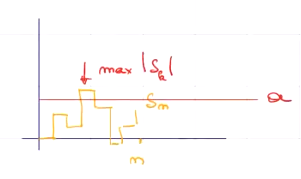
\includegraphics[width=0.6\linewidth]{screenshot017}
		\caption{The maximum of the random walk.}
		\label{fig:screenshot017}
	\end{figure}
	About this, we know that $\{S_{n}\}$ is a $\F$-martingale but in proving the Kolmogorov's inequaility we never talked about the martingale property! We could improve this inequality using the \emph{Doob's martingale inequality}. The problem is that we can prove very general inequalities that hold true for any \rv s but specifying more characteristic we can obtain stricter bounds. In this framework let's define 
	\begin{equation*}
		\begin{array}{l}
			M^{\star}_{n}=\max_{k\leq n}M_{k}\\
			m^{\star}_{n}=\min_{k\leq n}M_{k}\\
		\end{array}
	\end{equation*}
	as current maximum and current minimum of $M$.
	\begin{theorem}
		Take $M$ as a sub-martingale. For $b>0$ it holds:
		\begin{enumerate}
			\item $b\pr(M^{\star}_{n}\geq b)\leq\ev\left[M_{n}\indi_{\{M_{n}^{\star}\geq b\}}\right]\leq\ev\left[M_{n}^{+}\right]$;
			\item $b\pr(m^{\star}_{n}\leq-b)\leq-\ev M_{0}+\ev\left[M_{n}\indi_{\{m_{n}^{\star}\geq b\}}\right]\leq\ev M_{n}^{+}-\ev M_{0}$.
		\end{enumerate}
	\end{theorem}
	So we can further bound the result looking into the property of $M_{n}$.
	\begin{example}
		Now need to define the brownian motion (or Weiner process).
		\begin{definition}
			A real-valued stochastic process $B={(B_{t})}_{t\geq0}$ is called \emph{brownian motion} if:
			\begin{enumerate}
				\item the index set is $\R^{+}$;
				\item $B_{0}(\omega)=0$ for almost all $\omega$;
				\item $B_{t_{n}}-B_{t_{n-1}},\ldots,B_{t_{1}}-B_{t_{0}}$ are independent for $\every 0=t_{0}<t_1<\ldots<t_n<\infty$;
				\item $B_{t}-B_{s}\sim B_{t+b}-B_{s+b}$ for every $0\leq s<t<\infty\quad\every n>- s$;
				\item $B_{t}-B_{s}\sim N(0,t-s)$;
				\item $t\mapsto B_{t}(\omega)$ are continuous for every $\omega$.
			\end{enumerate}
		\end{definition}
		The brownian motion is in itself a martingale, but there is a class of martingales strictly related to it:
		\begin{equation*}
			M_{t}=\exp\left\{\lambda B_{t}-\frac{1}{2}\lambda^{2}t\right\},\qquad t\in\R^{+}.
		\end{equation*}
		Now we can get to the actual example: if $B$ is a brownian motion, we have 
		\begin{equation*}
			\pr(\sup_{0\leq t\leq\theta}B_{t}\geq b)\leq\exp\left\{-\frac{b^{2}}{s\theta}\right\}.
		\end{equation*}
		The sample paths of brownian motions are extremely irregular. We are asking with which probability the max of our process will be over $b$ at time $\theta$.
		\begin{figure}[H]
			\centering
			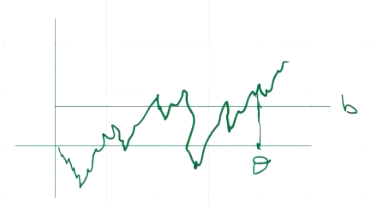
\includegraphics[width=0.6\linewidth]{screenshot018}
			\label{fig:screenshot018}
		\end{figure}
		I am basically asking if the maximum attained is above or below $b$.
		How can we use the Doob's inequality?
		\begin{fancyproof}
			Consider
			\begin{equation*}
				\pr(\sup B_{t}\geq b)=\pr(\sup e^{\lambda B_{t}}\geq e^{\lambda b})
			\end{equation*}
			and using Doob's inequality
			\begin{align*}
				\pr(\sup B_{t}\geq b)&=\pr(\sup e^{\lambda B_{t}}\geq e^{\lambda b})\\
				&\leq \frac{\overbrace{\ev\left[e^{\lambda B_{\theta}-\frac{\lambda^{2}}{2}\theta}\right]}^{\text{martingale}}}{e^{\lambda b}e^{-\frac{\lambda^{2}}{2}\theta}}\\
				&=e^{-\lambda b+\frac{\lambda^{2}}{2}\theta}\qquad\every\lambda>0
			\end{align*}
		\end{fancyproof}
	\end{example}
	\subsection{Predictable processes and Doob’s decomposition}
	\begin{definition}
		The process $F={(F_{n})}_{n\geq1}$ is \emph{$\F$-predictable} if $F_{0}\in\F_{0}$ and $\F_{n+1}\in\F_{n}$, for $\every n\in\N$.
	\end{definition}
	This means that the available information up to $n$ is ``enough'' to have a bet in the period $n+1$. Some predictable processes are:
	\begin{itemize}
		\item any deterministic processes;
		\item consider two stopping times $S,T$ of $\F$ and let $S\leq T$. Consider the \rv{} $V$ in $\F_{n}$. Then
		\[\begin{array}{c c c c}
			\color{DodgerBlue3}(1)&\color{DodgerBlue3}(2)&\color{DodgerBlue3}(3)&\color{DodgerBlue3}(4)\\
			V\indi_{(S,T]}&V\indi_{(S,\infty]}&\indi_{(S,T]}&\indi_{(0,T]}
		\end{array}\]
		are predictable processes.
		\begin{fancyproof}
			\begin{enumerate}
				\item[\color{DodgerBlue3}(2)] Consider $F=V\indi_{(S,\infty]}$, so that $F_{n}=\indi_{(S,\infty]}(n)$. Consider \begin{align*}
					F_{n+1}&=V\indi_{(S,\infty]}(n+1)\\
					&=V\indi_{\{S<n+1\}}\\
					&=V\indi_{\{S\leq n\}}\in\F_{n}
				\end{align*}
				so the process is $\F$-measurable and predictable.
				\item[\color{DodgerBlue4}(1)] Since we know by hypothesis that $S\leq T$ then $V\in\F_{S}\subset\F_{T}$. This means that $V\in\F_{T}$. Hence, of a consequence,
				\begin{equation*}
					V\indi_{(T,\infty]}-V\indi_{(S,\infty]}=V\indi_{(S,T]}
				\end{equation*}
				is predictable.
				\item[\color{DodgerBlue3}(3)] Take $V=1$.
				\item[\color{DodgerBlue3}(4)] Take $T=\infty$, $V=1$. $\indi_{(S,\infty]}$ is predictable. But then 
				\[\indi_{[0,S]}=\indi-\indi_{(S,\infty]}\]
				so it is predictable.
			\end{enumerate}
		\end{fancyproof}
	\end{itemize}
	\begin{theorem}
		\emph{Doob's decomposition}.\\
		$X$ is a stochastic process which is adapted to $\F$ and integrable. Then
		\begin{enumerate}
			\item it can be decomposed as 
			\[X_{n}=X_{0}+M_{n}+A_{n},\qquad n\in\N\]
			where:
			\begin{itemize}
				\item $M_{n}$ is a $\F$-martingale with $M_0=0$;
				\item $A_{n}$ is a predictable process with $A_0=0$.
			\end{itemize}
			\item The decomposition is unique up to equivalence.
			\item If $X_{n}$ is a sub-martingale then ${\{A_{n}\}}_{n\geq0}$ increasing, while if $X_{n}$ is a super-martingale then ${\{A_{n}\}}_{n\geq0}$ is decreasing.
		\end{enumerate}
	\end{theorem}
	\begin{fancyproof}
		Put $A_0=M_0=0$. Define $M$ and $A$ through their increments:
		\[ \begin{array}{l l}
			A_{n+1}-A_{n}&=\underbracket[0.3pt]{\ev\Big[X_{n+1}-X_{n}|\F_{n}\Big]}_{\F_{n}-\text{meas.}}\\
			M_{n+1}-M_{n}&=(X_{n+1}-X_{n})-(A_{n+1}-A_{n}).
		\end{array} \]
		If we look at these quantities we see that $A$ is predictable and $M$ is martingale. Imagine now there is another decomposition: let
		\[X=X_0+M'+A'\]
		be another decomposition. We must have
		\[\cancel{X_0}+M'+A'=\cancel{X_0}+M+A\iff A-A'=M-M'=B.\]
		Now $B$ is a process and it is predictable and martingale (because it is the difference between two martingales). Since $B$ is predictable \textit{and} a martingale we have
		\begin{align*}
			B_{n+1}-B_{n}&\underset{\mathclap{\text{\tiny predictable}}}{=}\ev[B_{n+1}-B_{n}|\F_{n}]\\
			&\underset{\mathclap{\text{\tiny martingale}}}{=}0\\
			&\implies B_{n+1}=B_{n}=B_0\;\as,A=A'\;\as,M=M'\as\\
		\end{align*}
		If $X$ is a sub-martingale then we have
		\[\ev[X_{n+1}-X_{n|\F_{n}}]\geq0\]
		and this means that we have $A_{n+1}\geq A_{n}$ is increasing.
	\end{fancyproof}
	\subsection{Doob’s stopping theorem}
	For a martingale we know
	\[\ev[X_{t}-X_{s}|\F_{s}]=0.\]
	The question is: is this true also if $s$ and $t$ are substituted by stopping times $S,T,S\leq T$?
	\begin{theorem}
		Let $M$ be adapted to $\F$. Then the following are equivalent:
		\begin{enumerate}[\circnum]
			\item $M$ is a submartingale;
			\item for every bounded stopping time $S\leq T$ the \rv s $M_{S}$ and $M_{T}$ are integrable and 
			\[\ev[M_{T}-M_{S}|\F_{S}]\geq0;\]
			\item for each pair of bounded stopping times the \rv s $M_{S}$ and $M_{T}$ are integrable and 
			\[\ev[M_{T}-M_{S}]\geq 0.\] 
		\end{enumerate}
	\end{theorem}
	\begin{remark}
		If $M$ is a martingale the theorem can be read in a different way:
		\begin{equation*}
			\ev M_{T}=\ev M_{S}=\ev M_{0}.
		\end{equation*}
		Previously, $\ev M_{n}=\ev M_{n-1}=\ev M_{0}$.
	\end{remark}
	\begin{fancyproof}
		To prove the theorem we need to show that from condition 1 follows 2 from which follows 3 from which follows 1.
		\begin{enumerate}
			\item[$1\to 2$] by hypothesis $M$ is a sub-martingale and our thesis is that if $S(\omega)<T(\omega)<n$ (because we asked for bounded times) then:
			\begin{enumerate}
				\item $M_{S}$ and $M_{T}$ are integrable;
				\item $\ev[M_{T}-M_{S}|\F_{S}]\geq0$.
			\end{enumerate}
			We know that $S$ and $T$ are bounded by $n$. Let $V$ be a positive bounded \rv{} and define $F=V\indi_{(S,T]}$ and use it in the discrete time integral:
			\[X_{n}=\underbrace{M_0F_0}_{X_0}+(M_1-M_0)\underbrace{F_1}_{\mathclap{V\indi_{\{1\in(S,T]\}}}}+\ldots+(M_{n}-M_{n-1})F_{n}\]
			So we have 
			\[X_{n}-X_{0}=V(M_{T}-M_{S})\]
			So $X_{n}$ is a sub-martingale. Take $V=1$ and $S=0$: now we have
			\begin{equation*}
				\begin{array}{c c c l}
					X_{n}&-&X_{0}&=M_{T}\\
					\downarrow&&\downarrow&\\
					\text{int.}&&\text{int.}&\implies M_{T}\text{ is integrable}.
				\end{array}
			\end{equation*}
			Now take $V=1$ and $T=n$ so that we get
			\begin{equation*}
				\begin{array}{c c c c l}
					X_{n}&-&X_{0}&=M_{n}&-M_{S}\\
					\downarrow&&\downarrow&\downarrow&\\
					\text{int.}&&\text{int.}&\text{int.}&\implies M_{S}\text{ is integrable}.
				\end{array}
			\end{equation*}
			We recall that $V\in\F_S$ and we use the defining property for $\ev(\cdot|\F_S)$. So we can write
			\begin{align*}
				\ev V\ev(M_{T}-M_{S}|\F_{S})&\underset{\mathclap{\text{def. prop.}}}{=}\ev V(M_{T}-M_{S})\\
				&\underset{\mathllap{\text{discr. time int.}}}{=}\ev[X_{n}-X_{0}]\\
				&\underset{\mathllap{\text{proved above}}}{\geq}0
			\end{align*}
			and this is true $\every V>0,V<b,V\in\F_{s}$. Hence
			\begin{equation*}
				\ev(M_{T}-M_{S}|\F_{S})\geq 0
			\end{equation*}
			So $1\to2$.
			\item[$2\to3$] We can use the tower rule. Take the expectation of point 2:
			\[\ev[\ev(M_{T}-M_{S}|\F_{S})]=\ev[M_{T}-M_{S}]\geq0.\]
			\item[$3\to1$] Let $3$ hold, so that $\ev[M_{T}-M_{S}]\geq0$. Choose $T=n$ and $S=0$. Then
			$M_{n}$ is integrable. Move to adaptness: this holds by hypothesis. Move to the martingale inequality:
			\begin{equation*}
				\ev[M_{n}-M_{m}|\F_{m}]\geq0.
			\end{equation*}
			Note that this is equivalent to prove 
			\begin{equation*}
				\ev\indi_H\ev[M_{n}-M_{m}|\F_{m}]\geq0\qquad H\in\F_{m},0\leq m\leq n.
			\end{equation*}
			Fix $H,m,n$ and define
			\begin{equation*}
				S(\omega)=m\qquad T(\omega)=n\indi_H(\omega)+m\indi_{\{\Omega\setminus H\}}(\omega)
			\end{equation*}
			The indicators are non-zero in complementary instances. Notice that:
			\begin{enumerate}
				\item $S$ is a fixed time so it is a stopping time;
				\item $S\leq T\leq n$ by definition of $S$ and $T$ because the indicators are non-zero in complementary instances;
				\item $T\geq S$ is a foretold time by $S=m$;
				\item $H\in\F_{S}$ by definition.
			\end{enumerate}
			So we can write $M_{T}-M_{S}=\indi_H(M_{n}-M_{m})$ where $M_{T}-M_{S}\geq0$ by hypothesis. This means that we have 
			\begin{equation*}
				\underbrace{\ev[\indi_{H}\ev(M_{n}-M_{m}|\F_{m})]}_{\ev[M_{n}-M_{m}|\F_{m}]\geq0}\geq0
			\end{equation*}
		\end{enumerate}
	\end{fancyproof}
	\subsection{Upcrossing inequality} 
	I believe that what is being asked is
	\begin{proposition}
		If $M$ is a sub-martingale with respect to its natural filtration then 
		\begin{equation*}
			(b-a)\ev U_{n}(a,b)\leq\ev\left[(M_{n}-a)^{+}-(M_{0}-a)^{+}\right].
		\end{equation*}
	\end{proposition}
	We wanted to find a bound for our profit, but our profit is a stochastic quantity: so it's only natural to think about the expectation to give a bound to the number of expected up/downcrossing.\\
	Observe that the number of upcrossings does not depend on the value of $T_0$ that we fix.
	\begin{fancyproof}
		Choose $a=0$. Consider hence the process $(M-a)^{+}$ that is sub-martingale (if $M$ is a sub-martingale). Take $M\geq 0$ and let 
		\begin{equation*}
			F_{n}=\indi_{(S_{k},T_{k}]}(n)
		\end{equation*}
		and consider 
		\begin{equation*}
			X=\int F\dif M
		\end{equation*}
		like in our example. We know that $F$ is predictable since by definition $F_{k+1}\in\F_{k}$. Consider the expectation of the increment
		\begin{equation*}
			\ev[X_{k+1}-X_{k}|\F_{k}]=\ev\left[F_{k+1}(M_{k+1}-M_{k})|\F_{k}\right].
		\end{equation*}
		But since $F_{k+1}$ is predictable we can take it out the expectation:
		\begin{equation*}
			F_{k+1}\ev\left[M_{k+1}-M_{k}|\F_{k}\right].
		\end{equation*}
		But since $F_{k+1}$ is an indicator we know it is $\leq1$:
		\begin{equation*}
			\ev[X_{k+1}-X_{k}|\F_{k}]\leq\ev\left[M_{k+1}-M_{k}|\F_{k}\right].
		\end{equation*}
		Now take the expectation of both sides:
		\begin{equation*}
			\ev[X_{k+1}-X_{k}]\leq\ev\left[M_{k+1}-M_{k}\right].
		\end{equation*}
		If we sum these inequalities over $k$ we get:
		\begin{equation*}
			\ev\left[X_{n}-X_{0}\right]\leq\ev\left[M_{n}-M_{0}\right].
		\end{equation*}
		So we now get that
		\begin{equation*}
			bU_{n}(a,n)\leq\ev\left[X_{n}-X_{0}\right]\leq\ev\left[M_{n}-M_{0}\right]
		\end{equation*}
		but given that $a=0$ we get that
		\begin{equation*}
			bU_{n}(0,b)\leq\ev[M_{n}-M_{0}].
		\end{equation*}
		Clearly we have to take the positive part.
	\end{fancyproof}
	But I also found this
	\begin{proposition}
		Suppose that $\{X={X_{t}:t\in[0,\infty)}\}$ satisfies the basic assumptions with respect to the filtration $\F=\{\F_t:t\in[0,\infty)\}$ and let $a,b\in\R$ with $a<b$. Let $U_{t}=u_{t}(a,b,X)$ the random number of upcrossings of $[a,b]$ by $X$ up to time $t\in[0,\infty)$. 
		\begin{enumerate}[\circnum]
			\item if $X$ is a super-martingale relative to $\F$ then
			\begin{equation*}
				\ev(U_{t})\leq\frac{1}{b-a}\ev\left[(X_{t}-a)^{-}\right]\leq\frac{1}{b-a}\left[\ev(X_{t}^-)+|a|\right]\leq\frac{1}{b-a}\left[\ev(|X_{t}|)+|a|\right];
			\end{equation*}
			\item if $X$ is a sub-martingale relative to $\F$ then
			\begin{equation*}
				\ev(U_{t})\leq\frac{1}{b-a}\ev\left[(X_{t}-a)^{+}\right]\leq\frac{1}{b-a}\left[\ev(X_{t}^+)+|a|\right]\leq\frac{1}{b-a}\left[\ev(|X_{t}|)+|a|\right];
			\end{equation*}
		\end{enumerate}	
	\end{proposition}
	\subsection{Doob’s decomposition}
	\begin{theorem}
		\emph{Doob's decomposition}.\\
		$X$ is a stochastic process which is adapted to $\F$ and integrable. Then
		\begin{enumerate}
			\item it can be decomposed as 
			\[X_{n}=X_{0}+M_{n}+A_{n},\qquad n\in\N\]
			where:
			\begin{itemize}
				\item $M_{n}$ is a $\F$-martingale with $M_0=0$;
				\item $A_{n}$ is a predictable process with $A_0=0$.
			\end{itemize}
			\item The decomposition is unique up to equivalence.
			\item If $X_{n}$ is a sub-martingale then ${\{A_{n}\}}_{n\geq0}$ increasing, while if $X_{n}$ is a super-martingale then ${\{A_{n}\}}_{n\geq0}$ is decreasing.
		\end{enumerate}
	\end{theorem}
	\begin{fancyproof}
		Put $A_0=M_0=0$. Define $M$ and $A$ through their increments:
		\[ \begin{array}{l l}
			A_{n+1}-A_{n}&=\underbracket[0.3pt]{\ev\Big[X_{n+1}-X_{n}|\F_{n}\Big]}_{\F_{n}-\text{meas.}}\\
			M_{n+1}-M_{n}&=(X_{n+1}-X_{n})-(A_{n+1}-A_{n}).
		\end{array} \]
		If we look at these quantities we see that $A$ is predictable and $M$ is martingale. Imagine now there is another decomposition: let
		\[X=X_0+M'+A'\]
		be another decomposition. We must have
		\[\cancel{X_0}+M'+A'=\cancel{X_0}+M+A\iff A-A'=M-M'=B.\]
		Now $B$ is a process and it is predictable and martingale (because it is the difference between two martingales). Since $B$ is predictable \textit{and} a martingale we have
		\begin{align*}
			B_{n+1}-B_{n}&\underset{\mathclap{\text{\tiny predictable}}}{=}\ev[B_{n+1}-B_{n}|\F_{n}]\\
			&\underset{\mathclap{\text{\tiny martingale}}}{=}0\\
			&\implies B_{n+1}=B_{n}=B_0\;\as,A=A'\;\as,M=M'\as\\
		\end{align*}
		If $X$ is a sub-martingale then we have
		\[\ev[X_{n+1}-X_{n|\F_{n}}]\geq0\]
		and this means that we have $A_{n+1}\geq A_{n}$ is increasing.
	\end{fancyproof}
	\subsection{Stochastic integral in discrete time}
	Let us consider two real-valued processes $M={(M_{n})}_{n}$ and $F={(F_{n})}_{n}$ and let us define
	\[X_{n}=F_0M_{0}+(M_1-M_0)F_1+\ldots+(M_{n}-M_{n-1})F_n.\]
	We say that $\{X_{n}\}$ is the integral of $F$ with respect to $M$ and we write
	\[X_{n}=\int F \dif M\]
	where $\dif M$ is a random signed measure. Remember the Lebesgue-Stieltjes integral? Me neither, but as long as $M$ has bounded variation this is a Lebesgue-Stieltjes integral. So a little explanation is due since I actually never saw a Stieltjes integral.
	\begin{theorem}
		Consider $F$ bounded and predictable. Then if $M$ is a martingale then $X$ is a martingale; If $M$ is a sub(super)-martingale then $X$ is a sub(super)-martingale.
	\end{theorem}
	This means that... \emph{we can't beat the system!}
	\begin{flushright}
		\begin{tikzpicture}
			\calloutquote[width=4cm,position={(1,-1)},fill=Turquoise4!30,rounded corners]{I can beat something else though.}
		\end{tikzpicture}\hspace*{2.5cm}
	\end{flushright}
	\begin{example}
		Consider $M_{n}$ as the price of a share at time $n$ and $F_{n}$ as the number of shares owned during $(n-1,n]$. Our profit will be 
		\[(M_{n}-M_{n=1})F_{n}\]
		and our total profit $X_{n}$ gained during $(0,n]$ will be:
		\[X_{n}=X_{0}+\underbrace{\sum_{k=1}^{n}(M_{k}-M_{k-1})F_{k}}_{\mathclap{\text{discrete time integral}}}\]
		$F_{n}$ is based on the knowledge in $n-1$ so it is predictable. The process $M_{n}$ should be a martingale (otherwise if it is a sub/super-martingale everyone/no one will buy). So the total profit will also be a martingale! We can only choose our buying politics $F_{k}$, but there is no way to select a politics that will change a martingale in a super-martingale or sub-martingale.
	\end{example}
	Clearly this works in mean! 
	\begin{fancyproof}
		\begin{enumerate}
			\item	We have $M$ being a martingale and $F_0,F_1,\ldots,F_n\in\F_{n}$ as well as $M_0,M_1,\ldots,M_{n}\in\F_n$. Therefore $X_{n}\in\F_{n}$ and $X$ is adapted to $\F$.
			\item We need to check whether the discrete time integral is a martingale. We know by hypothesis that $F$ is bounded, so $F<b$ for some $b$. This implies
			\begin{equation*}
				|X_{n}|<b(|M_{0}|+|M_1+M_0|+\ldots+|M_n-M_{n-1}|)
			\end{equation*}
			Since $M$ is a martingale and it is integrable, we get that $X_n$ is bounded and integrable.
			\item Consider
			\begin{equation*}
				\ev[X_{n+1}-X_{n}|\F]=\ev[F_{n+1}(M_{n+1}-M_{n})|\F_n]
			\end{equation*}
			since all the terms cancel out and only the last ones survive. But $F_{n+1}\in\F_{n}$ so we can take it out of the expectation:
			\[F_{n}\underbrace{\ev[M_{n+1}-M_{n}|\F_{n}]}_{=0}=0.\]
		\end{enumerate}
	\end{fancyproof}
	\subsection{Stochastic integral and its application}
	Let us consider two real-valued processes $M={(M_{n})}_{n}$ and $F={(F_{n})}_{n}$ and let us define
	\[X_{n}=F_0M_{0}+(M_1-M_0)F_1+\ldots+(M_{n}-M_{n-1})F_n.\]
	We say that $\{X_{n}\}$ is the integral of $F$ with respect to $M$ and we write
	\[X_{n}=\int F \dif M\]
	where $\dif M$ is a random signed measure. Remember the Lebesgue-Stieltjes integral? Me neither, but as long as $M$ has bounded variation this is a Lebesgue-Stieltjes integral. So a little explanation is due since I actually never saw a Stieltjes integral.
	\begin{theorem}
		Consider $F$ bounded and predictable. Then if $M$ is a martingale then $X$ is a martingale; If $M$ is a sub(super)-martingale then $X$ is a sub(super)-martingale.
	\end{theorem}
	This means that... \emph{we can't beat the system!}
	\begin{flushright}
		\begin{tikzpicture}
			\calloutquote[width=4cm,position={(1,-1)},fill=Turquoise4!30,rounded corners]{I can beat something else though.}
		\end{tikzpicture}\hspace*{2.5cm}
	\end{flushright}
	\begin{example}
		Consider $M_{n}$ as the price of a share at time $n$ and $F_{n}$ as the number of shares owned during $(n-1,n]$. Our profit will be 
		\[(M_{n}-M_{n=1})F_{n}\]
		and our total profit $X_{n}$ gained during $(0,n]$ will be:
		\[X_{n}=X_{0}+\underbrace{\sum_{k=1}^{n}(M_{k}-M_{k-1})F_{k}}_{\mathclap{\text{discrete time integral}}}\]
		$F_{n}$ is based on the knowledge in $n-1$ so it is predictable. The process $M_{n}$ should be a martingale (otherwise if it is a sub/super-martingale everyone/no one will buy). So the total profit will also be a martingale! We can only choose our buying politics $F_{k}$, but there is no way to select a politics that will change a martingale in a super-martingale or sub-martingale.
	\end{example}
	Clearly this works in mean! 
	\begin{fancyproof}
		\begin{enumerate}
			\item	We have $M$ being a martingale and $F_0,F_1,\ldots,F_n\in\F_{n}$ as well as $M_0,M_1,\ldots,M_{n}\in\F_n$. Therefore $X_{n}\in\F_{n}$ and $X$ is adapted to $\F$.
			\item We need to check whether the discrete time integral is a martingale. We know by hypothesis that $F$ is bounded, so $F<b$ for some $b$. This implies
			\begin{equation*}
				|X_{n}|<b(|M_{0}|+|M_1+M_0|+\ldots+|M_n-M_{n-1}|)
			\end{equation*}
			Since $M$ is a martingale and it is integrable, we get that $X_n$ is bounded and integrable.
			\item Consider
			\begin{equation*}
				\ev[X_{n+1}-X_{n}|\F]=\ev[F_{n+1}(M_{n+1}-M_{n})|\F_n]
			\end{equation*}
			since all the terms cancel out and only the last ones survive. But $F_{n+1}\in\F_{n}$ so we can take it out of the expectation:
			\[F_{n}\underbrace{\ev[M_{n+1}-M_{n}|\F_{n}]}_{=0}=0.\]
		\end{enumerate}
	\end{fancyproof}
	and for the applications:\\
	\begin{definition}
		Define $M={(M_{n})}_{n\in\N}$ as a process and let $T$ be a random time with values on $\overline{\N}$. The process
		\[X_{n}(\omega)=M_{n\wedge T}(\omega)=\begin{cases}
			M_{n}(\omega)&n<T(\omega)\\
			M_{T}(\omega)&n>T(\omega)
		\end{cases}\]
		(where $n\wedge T$ is a truncated random time) is called \emph{$M$ stopped at $T$}.
	\end{definition}
	As a consequence $X$ is exactly the discrete time integral if $F=\indi_{[0,T]}$:
	\begin{equation*}
		X_{n}=\underbracket[0.6pt]{M_0F_0}_{0}+(M_{1}+M_{0})\indi_{[0,T]}(1)+\ldots+(M_{n}-M_{n-1})\indi_{[0,T]}(n).
	\end{equation*}
	The indicators only select the current time interval. If this is the case we can observe that $F_{[0,T]}$ is bounded, positive and predictable. Hence if $M$ is a martingale the theorem applies with this special choice of $M$ and we can write the result as a different theorem:
	\begin{theorem}
		Let $T$ be a stopping time and let $X$ be the process $M$ stopped at $T$. If $M$ is a martingale then so is $X$ (the same holds for sub-martingales and super-martingales).
	\end{theorem}
	So we cannot determine a policy based on stopping times that can change the nature of our martingale. In the remote case in which you are interested in this you can read Williams - Introduction to martingales. \\
	\subsection{Impossibility to win against the system: related theorems and examples}
	\begin{theorem}
		Consider $F$ bounded and predictable. Then if $M$ is a martingale then $X$ is a martingale; If $M$ is a sub(super)-martingale then $X$ is a sub(super)-martingale.
	\end{theorem}
	This means that... \emph{we can't beat the system!}
	\begin{flushright}
		\begin{tikzpicture}
			\calloutquote[width=4cm,position={(1,-1)},fill=Turquoise4!30,rounded corners]{I can beat something else though.}
		\end{tikzpicture}\hspace*{2.5cm}
	\end{flushright}
	\begin{example}
		Consider $M_{n}$ as the price of a share at time $n$ and $F_{n}$ as the number of shares owned during $(n-1,n]$. Our profit will be 
		\[(M_{n}-M_{n=1})F_{n}\]
		and our total profit $X_{n}$ gained during $(0,n]$ will be:
		\[X_{n}=X_{0}+\underbrace{\sum_{k=1}^{n}(M_{k}-M_{k-1})F_{k}}_{\mathclap{\text{discrete time integral}}}\]
		$F_{n}$ is based on the knowledge in $n-1$ so it is predictable. The process $M_{n}$ should be a martingale (otherwise if it is a sub/super-martingale everyone/no one will buy). So the total profit will also be a martingale! We can only choose our buying politics $F_{k}$, but there is no way to select a politics that will change a martingale in a super-martingale or sub-martingale.
	\end{example}
	Clearly this works in mean! 
	\begin{fancyproof}
		\begin{enumerate}
			\item	We have $M$ being a martingale and $F_0,F_1,\ldots,F_n\in\F_{n}$ as well as $M_0,M_1,\ldots,M_{n}\in\F_n$. Therefore $X_{n}\in\F_{n}$ and $X$ is adapted to $\F$.
			\item We need to check whether the discrete time integral is a martingale. We know by hypothesis that $F$ is bounded, so $F<b$ for some $b$. This implies
			\begin{equation*}
				|X_{n}|<b(|M_{0}|+|M_1+M_0|+\ldots+|M_n-M_{n-1}|)
			\end{equation*}
			Since $M$ is a martingale and it is integrable, we get that $X_n$ is bounded and integrable.
			\item Consider
			\begin{equation*}
				\ev[X_{n+1}-X_{n}|\F]=\ev[F_{n+1}(M_{n+1}-M_{n})|\F_n]
			\end{equation*}
			since all the terms cancel out and only the last ones survive. But $F_{n+1}\in\F_{n}$ so we can take it out of the expectation:
			\[F_{n}\underbrace{\ev[M_{n+1}-M_{n}|\F_{n}]}_{=0}=0.\]
		\end{enumerate}
	\end{fancyproof}
	We know that using a policy that it is predictable it is impossible to beat the system. Finance bros try to overcome this possibility using stopping times. If my policy is not only based on a predictable process but I add the randomness of the time in which I decide to sell or buy can I break the curse of martingales and make shareholders want to suck my dick? Well, it depends.
	\subsection{Predictable and adapted processes: definition and examples}
	\begin{definition}
		The process $F={(F_{n})}_{n\geq1}$ is \emph{$\F$-predictable} if $F_{0}\in\F_{0}$ and $\F_{n+1}\in\F_{n}$, for $\every n\in\N$.
	\end{definition}
	This means that the available information up to $n$ is ``enough'' to have a bet in the period $n+1$. Some predictable processes are:
	\begin{itemize}
		\item any deterministic processes;
		\item consider two stopping times $S,T$ of $\F$ and let $S\leq T$. Consider the \rv{} $V$ in $\F_{n}$. Then
		\[\begin{array}{c c c c}
			\color{DodgerBlue3}(1)&\color{DodgerBlue3}(2)&\color{DodgerBlue3}(3)&\color{DodgerBlue3}(4)\\
			V\indi_{(S,T]}&V\indi_{(S,\infty]}&\indi_{(S,T]}&\indi_{(0,T]}
		\end{array}\]
		are predictable processes.
		\begin{fancyproof}
			\begin{enumerate}
				\item[\color{DodgerBlue3}(2)] Consider $F=V\indi_{(S,\infty]}$, so that $F_{n}=\indi_{(S,\infty]}(n)$. Consider \begin{align*}
					F_{n+1}&=V\indi_{(S,\infty]}(n+1)\\
					&=V\indi_{\{S<n+1\}}\\
					&=V\indi_{\{S\leq n\}}\in\F_{n}
				\end{align*}
				so the process is $\F$-measurable and predictable.
				\item[\color{DodgerBlue4}(1)] Since we know by hypothesis that $S\leq T$ then $V\in\F_{S}\subset\F_{T}$. This means that $V\in\F_{T}$. Hence, of a consequence,
				\begin{equation*}
					V\indi_{(T,\infty]}-V\indi_{(S,\infty]}=V\indi_{(S,T]}
				\end{equation*}
				is predictable.
				\item[\color{DodgerBlue3}(3)] Take $V=1$.
				\item[\color{DodgerBlue3}(4)] Take $T=\infty$, $V=1$. $\indi_{(S,\infty]}$ is predictable. But then 
				\[\indi_{[0,S]}=\indi-\indi_{(S,\infty]}\]
				so it is predictable.
			\end{enumerate}
		\end{fancyproof}
	\end{itemize} 
	Example of adapted process:
	\begin{example}
		This is called ``the secretary problem'': in this case we must start from the filtration and then understand the problem.
		Here i have $N$ candidates for a position; a candidate disregarded after the interview is lost. The interviewer wants to hire exactly 1 candidate and each candidate has different abilities and the interviewer knows only the relative ability of those already interviewed so far. Our goal is to maximizing the probability of hiring the best one. We have three questions:
		\begin{enumerate}
			\item what is $\Omega$?
			\item what is the filtration $\F$ for this experiment?
			\item what process should we use?
		\end{enumerate}
		In this case $\Omega=N!$ permutations of the ranking of the candidates (the order in which they show up) and the filtration is the information earned from interview up to time $t$ (that is the ranking of the candidates up to time $t$). But what is the process that I should use? Consider the sequence
		\[V_1,V_2,\ldots\qquad{\{V_i\}}_{i\geq 1}\]
		with $V_i=1$ if and only if the best candidate is the $i$-th candidate and $V_i=0$ otherwise. Could this process ${\{V_i\}}_{i\geq 1}$ be used? No, because $V$ is not adapted to $\F$... because to understand if $i$-th candidate is te best we need to compare it to the other candidates, including the ones that didn't show up yet! But then how can we get an adapted process? Let us consider the expectation
		\[U_n=\ev\left[V_n|\F_n\right]\]
		What do we know about the measurability of $U_n$? We know that it is for sure $\F_n$-measurable. This trick gives us a simple way to build an adapted process. So now we will have:
		$U_n=
		0$ if the candidate is not the best up to $n$ and $U_n=1$ otherwise. More specifically, we will have
		\begin{align*}
			U_n&=1\cdot\substack{\text{proability that the best candidate}\\\text{is among the first $n$}}+0\cdot\substack{\text{proability that the best candidate}\\\text{is not among the first $n$}}\\
			&=1\cdot\frac{n}{N}+0\cdot\frac{N-n}{N}.\\
			&=\frac{n}{N}
		\end{align*}
		This is a quantity that I can measure and it is therefore adapted.\par
	\end{example}
	\subsection{Poisson process and its martingale property}
	Consider $\R_+$ as our index set. $\F$ is our filtration and we consider the counting process $N={(N_{t})}_{y\geq0}$: this counts the number of events up to time $t$, it has unit jumps and any path starts from 0 so that $N_{0}(\omega)=0$, it is increasing and it is right continuous.
	\begin{definition}
		The counting process $N$ is said to be a \emph{Poisson process} with rate $\lambda$ with respect to $\F$ if it is adapted to $\F$ and
		\[\ev[f(N_{t+s}-N_s)|\F_s]=\sum_{k=0}^{\infty}e^{-\lambda t}\frac{(\lambda t)^{k}}{k!}f(k)\qquad\every s,t\in\R_+,\every\text{positive }f\mapsto\N.\]
	\end{definition}
	\begin{theorem}
		Let $N$ be a counting process. It is a Poisson process with rate $\lambda$ with respect to $\F$ \ifonly{}:
		\begin{equation*}
			M_{t}=N_{t}-\lambda t
		\end{equation*}
		is a $\F$-martingale.
	\end{theorem}
	We only prove that $M_t$ is a martingale if $N_{t}$ is Poisson.
	\begin{fancyproof}
		We know that 
		\begin{align*}
			\ev[M_{t}|\F_{s}]&=\ev[M_{t}-M_{s}+M_{s}|\F_{s}]\\
			&=\ev[M_{t}-M_{s}|\F_{s}]+M_{s}\\
			&=\ev[M_{t}-M_{s}]+M_{s}\\
			&=\ev[N_{t}-N_{s}+\lambda t+\lambda s]+M_{s}\\
			&=\underbrace{\ev[N_{t}-N_{s}]}_{\cancel{\lambda (t-s)}}-\cancel{\lambda (t-s)}+M_{s}\\
			&=M_{s}
		\end{align*}
	\end{fancyproof}
	\subsection{Stopped processes and their properties}
	\begin{example}
		Some stopping times:
		\begin{enumerate}[\circnum]
			\item The first time that $X(\omega)\in H\in\Omega$;
			\[T(\omega)=\begin{cases}
				\inf \left\{n\in\N:X_n(\omega)\in H\right\}&\\
				+\infty&\text{if $X_n(\omega)\notin H\;\every n$}
			\end{cases}\]
			So
			\[\left\{T\leq n\right\}=\bigcup_{k=0}^{n}\left\{X_k\in H\right\}.\]
			\item Consider i.i.d. \rv{}s 
			$X_1,X_2,\ldots$. Consider the probabilities
			\[\pr(X_i=1)=\pr(X_i=-1)=\frac{1}{2}\]
			and the random walk
			\[S_n=\sum_{1}^{n}X_i.\]
			Let's define 
			\[T_1=\begin{cases}
				\min\left\{n<50:S_n=3\right\}\\
				50 &\text{otherwise}.
			\end{cases}\]
			This is a stopping time because I can write $\left\{T_1\leq n\right\}$ as $$\underbracket[0.6pt]{\bigcup_{k=1}^{n}\underbracket[0.6pt]{\left\{S_k=3\right\}}_{\text{$\F_k$-measurable}}}_{\mathclap{\text{$\F_n$-measurbale}}}\qquad n<50.$$
			Moreover for $n=50$ we have $T_{1}\in\F_{50}$.
			\item Starting from the previously deifned random walk, consider the quantity 
			\[M_n=\min(S_1,\ldots,S_n)\]
			And the random time
			\[T_2=\min\left\{n:S_n\geq M_m+2\right\}\]
			is a stoppimg time. On the contrary, 
			\[T_3=\begin{cases}
				\max\left\{n<50:S_n=7\right\}&\text{if not empty}\\
				50 &\text{otherwise}
			\end{cases}\]
			is not a stopping time. Why? Because I have to wait until $n=50$ to answer the question. 
		\end{enumerate}
	\end{example}
	
	Consider the random times on $\R_+$
	\[0<T_1<T_2<\ldots\]
	With $\lim_{n\to\infty}T_n=+\infty$. Define the process $\left\{N_t\right\}$ as 
	\[N_t:=\sum\indi_{[0,t]}(T_n).\]
	This is called \emph{counting process}. It is a basic count of the number of events happened up to time $n$.
	$N_{t}$ is increasing, right continuous and incresases by unitary jumps. Moreover, $N_0=0$, $N_t<\infty$ for $t\in\R_+$. Of course $\lim_{t\to\infty}N_t=\infty$. Counting processes generate their natural filtration $\F$.
	
	Some problems require to stop the observation at a stopping time (because we don't care anymore\footnote{Assuming we ever did.})... So we don't actually need the whole knowledge of the complete filtration $\F={\left(\F_t\right)}_{t\geq 0}$. The problem is that as we said before the stopping time is a random time. So what we need is the \textit{information known up to time $T$} $\F_T$, basically the $\sigma$-field that is the filtration at time $T$. 
	\begin{example}
		\emph{Truncated stopping time}: let $T$ be a stopping time (for example, the time at which we sell certain shares) and that we want a finite horizon for this decision. In this case the quantity of interest is
		\begin{equation*}
			S=T\wedge n=\min\{T,n\}
		\end{equation*}
		where $n$ could be some sort of time horizon.\\
		Imagine that two cyclists participate to a race. Their children will have their snack when both the parents will arrive to the finish line. How long will the children wait for their snack?
		We can think about the following stopping times:
		\[ 	\begin{array}{l l}
			T: & \text{time employed by the first cyclist}\\
			S: & \text{time employed by the second cyclist}\\
			U: &\max\{S,T\}.
			
		\end{array} \]
		The waiting time for the children will be $U$.
	\end{example}
	\subsection{Important inequalities for sub-martingales}
	The problem is that we can prove very general inequalities that hold true for any \rv s but specifying more characteristic we can obtain stricter bounds. In this framework let's define 
	\begin{equation*}
		\begin{array}{l}
			M^{\star}_{n}=\max_{k\leq n}M_{k}\\
			m^{\star}_{n}=\min_{k\leq n}M_{k}\\
		\end{array}
	\end{equation*}
	as current maximum and current minimum of $M$.
	\begin{theorem}
		Take $M$ as a sub-martingale. For $b>0$ it holds:
		\begin{enumerate}
			\item $b\pr(M^{\star}_{n}\geq b)\leq\ev\left[M_{n}\indi_{\{M_{n}^{\star}\geq b\}}\right]\leq\ev\left[M_{n}^{+}\right]$;
			\item $b\pr(m^{\star}_{n}\leq-b)\leq-\ev M_{0}+\ev\left[M_{n}\indi_{\{m_{n}^{\star}\geq b\}}\right]\leq\ev M_{n}^{+}-\ev M_{0}$.
		\end{enumerate}
	\end{theorem}
	So we can further bound the result looking into the property of $M_{n}$.
	\begin{fancyproof}
		We introduce 2 stopping times: 
		\begin{equation*}
			\begin{array}{l l}
				T&=\inf\{n\geq0:M_{n}\geq b\}\\
				S&=\inf\{n\geq0:M_{n}\leq-b\}.
			\end{array}
		\end{equation*}
		\begin{figure}[H]
			\centering
			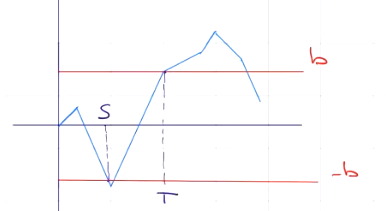
\includegraphics[width=0.6\linewidth]{screenshot019}
			\label{fig:screenshot019}
		\end{figure}
		Consider the current maximum and minimum above the level $b$:
		\begin{equation*}
			\{M^{\star}_{n}\geq b\}=\{T\leq n\}\qquad	\{m^{\star}_{n}<-b\}=\{S\leq n\}.
		\end{equation*}
		Fix $b$ and $n$. When $\{T\leq n\}$ we have
		\begin{align*}
			M_{T\wedge n}=M_{T}\geq b.
		\end{align*}
		Multiply by $\indi_{\{T\leq n\}}$:
		\begin{equation*}
			b\indi_{\{T\leq n\}}\leq M_{T\wedge n}\indi_{\{T\leq n\}}.
		\end{equation*}
		Using Doob's stopping theorem we know that 
		\begin{equation*}
			\ev\left[M_{T}-M_{S}|\F_{S}\right]\geq0
		\end{equation*}
		and using $S=T\wedge n$ and $T=n$ we obtain
		\begin{equation*}
			\ev\left[M_{n}|\F_{T\wedge n}\right]>M_{T\wedge n}.
		\end{equation*}
		So summing it all up:
		\begin{align*}
			b\indi_{\{T\leq n\}}&\leq M_{T\wedge n}\indi_{\{T\leq n\}}\\
			&\leq\indi_{\{T\leq n\}}\ev\left[M_{n}|\F_{T\wedge n}\right]\\
			&=\ev\left[M_{n}\indi_{\{T\leq n\}}|\F_{T\wedge n}\right].
		\end{align*}
		Now take the expectation:
		\begin{align*}
			b\pr(T\leq n)&=b\pr(M^{\star}_{n}\geq b)\\
			&\leq\underbrace{\ev\left[M_{n}\indi_{\{T\leq n\}}\right]}_{\mathclap{\ev\left[M_{n}\indi_{\{M_{n}^{\star}\geq b\}}\right]}}\\
			&\leq\ev(M^{+}_{n}).
		\end{align*}
		For the minimum we work on $\{S\leq n\}$ and we get 
		\begin{align*}
			M_{S\wedge n}&=M_{S}\indi_{\{S\leq n\}}+M_{S}\indi_{\{S>n\}}\\
			&\leq-b\indi_{\{S\leq n\}}+M_{n}\indi_{S\geq n}.
		\end{align*}
		Now take the expectation:
		\begin{equation*}
			\ev M_{S\wedge n}\leq-b\pr(m^{\star}_{n}\leq-b)+\ev\left[M_{n}\indi_{\{S>n\}}\right].
		\end{equation*}
		So that we get
		\begin{equation*}
			\pr(m^{\star}_{n}\leq-b)\leq-\ev M_{S\wedge n}+\ev[M_{n}\indi_{\{S>n\}}].
		\end{equation*}
		Now use Doob's stopping theorem with $T=0$ and $S=S\wedge n$ so that $\ev M_{0}\leq\ev M_{\{S\wedge n\}}$. This gets us our result:
		\begin{align*}
			b\pr(m^{\star}_{n}-b)&\leq-\ev M_{0}+\ev\left[M_{n}\indi_{\{m_{n}^{\star}\}}\right]\\
			&\leq\ev M^{+}_{n}-\ev M_{0}.
		\end{align*}
	\end{fancyproof}
	\subsection{Convergence theorems for sub-martingales}
	\begin{theorem}
		Let $X$ be a sub-martingale. If (and note that is a sufficient condition)
		\begin{equation*}
			\sup_{n}\ev X_{n}^{+}<\infty
		\end{equation*}
		Then
		\begin{enumerate}
			\item $\{X_{n}\}$ converges $\as$;
			\item $\{X_{n}\}$ converges to an integrable \rv.
		\end{enumerate}
	\end{theorem}
	\begin{fancyproof}
		We prove the theorem by contradiction. Pick an outcome $\omega$ and suppose that $\{X_{n}(\omega)\}$ is a numerical sequence that has not a limit. But if it doesn't have a limit, then 
		\[\exists\inf\lim\neq\sup\lim\qquad\inf\lim<\sup\lim.\]
		So there exist at least 2 rationals $a<b$ such that
		\begin{equation*}
			\inf\lim<a<b<\sup\lim.
		\end{equation*}
		The sequence $\{X_{n}(\omega)\}$ crosses $(a,b)$ $\infty$ many times. Now take the union over rational $a$ and $b$, $a<b$ of the sets
		\begin{equation*}
			\{U(a,b)=\infty\}
		\end{equation*}
		with $U(a,b)=\lim_{n\to\infty}U_{n}(a,b)$. Our aim is now to show that $U(a,b)\leq\infty$ almost surely to get a contradiction.\\
		Fix $a,b$. We know that $U_{n}(a,b)$ is increasing with $n$. Now consider
		\begin{align*}
			(b-a)\ev U(a,b)&=(b-a)\ev\lim U_{n}(a,b)\\
			&\underset{\mathclap{\text{monotone conv.}}}{=}(b-a)\lim\ev U_{n}(a,b)\\
			&\underset{\mathclap{\text{upcross inequalities}}}{\leq}\sup\ev(X_n-a)^{+}\\
			&\leq \sup\ev X_{n}^{+}+|a|.
		\end{align*}
		So this means that $\ev U(a,b)<\infty$. But this is a contradiction, so it exists a limit $X_{n}=X_{\infty}\as$.\\
		Now consider the second part of the theorem:
		\begin{align*}
			\ev|X_{\infty}|&=\ev\lim\inf|X_{n}|\\
			&\underset{\mathclap{\text{Fatou's lemma}}}{\leq}\lim\inf\ev|X_{n}|\\
			&\leq 2\sup\ev X_{n}^{+}-\ev X_{0}\leq\infty
		\end{align*}
		so the limit is integrable.
	\end{fancyproof}
	\subsection{Uniform integrability and its consequences on convergence of martingales}
	We will need:
	\begin{enumerate}
		\item a collection $\mathcal{K}$ of real \rv s is said to be uniformly integrable if 
		\begin{equation*}
			k(b)=\sup_{X\in\mathcal{K}}\ev|X|\indi_{\{X>b\}}\xrightarrow[b\to\infty]{}0.
		\end{equation*}
		\item If $\mathcal{K}$ is dominated by an integrable \rv{} $Z$ then it is uniformly integrable.
		\item uniform integrability implies $L^{1}$-boundedness but not the converse.
		\item If $\mathcal{K}$ is $L^{p}$-bounded for some $p>1$ then it is uniformly integrable.
	\end{enumerate}
	\begin{lemma}
		Let $Z$ be an integrable \rv{}. Then
		\begin{equation*}
			\mathcal{K}=\left\{X:X=\ev(Z|\G)\right\}
		\end{equation*}
		for some sub-\sa{} $\G$ of $\HS$ is uniformly integrable.
	\end{lemma}
	\begin{proposition}
		Let $Z$ be an integrable \rv{}. Define 
		\begin{equation*}
			X_{t}=\ev(Z|\F_{t})\qquad t\in\T.
		\end{equation*}
		This means that $\{X_{t}\}$ is a uniformly integrable $\F$-martingale.
	\end{proposition}
	\begin{theorem}
		Let $\{X_{n}\}$ be a sequence of real-valued \rv s. The following are equivalent:
		\begin{enumerate}
			\item it converges in $L^{1}$;
			\item it converges in probability and it is uniformly integrable.
		\end{enumerate}
	\end{theorem}
	We can now prove the theorem about the convergence of sub-martingales.
	\begin{theorem}
		Let $X$ be a sub-martingale. We have that $X$ converges almost surely and in $L^{1}$ \ifonly{} it is uniformly integrable. Moreover, if it is so, setting 
		\begin{equation*}
			X_{\infty}=\lim X_{n}
		\end{equation*}
		extends $X$ to a sub-martingale
		\begin{equation*}
			\xbar={(X_{n})}_{n\in\overline{\N}}.
		\end{equation*}
	\end{theorem}
	We only prove the first part of the theorem.
	\begin{fancyproof}
		\emph{Necessity}. If $X$ converges in $L^{1}$ by the theorem above it is uniformly integrable.\\
		\emph{Sufficiency}. If $X$ is uniformly integral then it is $L^{1}$-bounded for the property above. So our previous theorem holds and the martingale converges almost surely with $X_{\infty}$ integrable. Furthermore, for the property above, it also converges in $L^{1}$.
	\end{fancyproof}
	\subsection{Features of the sample paths of a submartingale (or martingale)}
	\begin{remark}
		If $M$ is a martingale then $|M|^{p}$ is a sub-martingale for $p\geq1$. If $M_{n}\in\lp\every n$ we can apply Doob's inequality.
	\end{remark}
	\begin{corollary}
		If $M$ is martingale in $\lp$ for some $p\geq 1$ then for $b>0$ we have that
		\begin{equation*}
			b^{p}\pr(\max_{k\leq n}|M_{k}|>b)\leq\ev|M_{n}|^{p}.
		\end{equation*}
	\end{corollary}
	There are also other bounds:
	\begin{itemize}
		\item $b\pr(\max_{k\leq n}|M_{k}>b)\leq 2\ev M_{n}^{+}-3M_{0}$;
		\item \emph{Doob's norm inequality}: if $M$ is a martingale in $\lp,p\geq 1$ and $q$ is the exponent conjugate to $p$ ($\frac{1}{p}+\frac{1}{q}=1$) then
		\begin{equation*}
			\ev\max_{  k\leq n}|M_{k}|^{p}\leq q^{p}\ev|M_{n}|^{p}.
		\end{equation*}
		\item  Consider $L^{2}$-bounded martingales characterized by final coordinate $X$ with $\var X=\sigma^{2}$ (that is I am fixing the variance of the last value I consider). We want to assess the variability of this process.
		\begin{theorem}
			\emph{Dubin \& Schwartz 1998}: it holds
			\begin{enumerate}
				\item $\ev\left[\max_{0\leq T\leq t}M_{T}\right]\leq\sigma$;
				\item $\ev\left[\max_{0\leq T\leq t}|M_{T}|\right]\leq\sigma\sqrt{2}$.
			\end{enumerate}
			Moreover, there exist suitable martingales for which this bound is attained and is scrict.
		\end{theorem}
	\end{itemize}
	\subsection{Uniform integrability and its role in convergence problems}
	\begin{theorem}
		A process $M={(M_{n})}_{n\in\N}$ is a uniformly integrable martingale \ifonly{} for some integrable \rv{} $Z$
		\begin{equation}
			M_{n}=\ev\left[Z|\F_{n}\right]\qquad n\in\N.\tag{$\bullet$}\label{AAAA}
		\end{equation}
		If so it converges almost surely and in $L^{1}$ to the integrable \rv
		\begin{equation*}
			M_{\infty}=\ev[Z|\F_{\infty}].
		\end{equation*}
	\end{theorem}
	\begin{corollary}
		For every integrable \rv{} $Z$ we have
		\begin{equation*}
			\ev(Z|\F_{n})\convas\xrightarrow[]{L^{1}}\ev(Z|\F_{\infty}).
		\end{equation*}
	\end{corollary}
	\begin{theorem}
		Let $Z$ be an integrable \rv{} and let 
		\begin{equation*}
			M_{n}=\ev(Z|\F_{n})_{n\in\overline{\N}}.
		\end{equation*}
		For every stopping time $T$ define
		\begin{equation*}
			M_{T}=\ev[Z|\F_{T}]
		\end{equation*}
		and for arbitrary stopping times $S$ and $T$ we get
		\begin{equation*}
			\ev[M_{T}|\F_{S}]=M_{S\wedge T}.
		\end{equation*}
	\end{theorem}
	This lets us rethink Doob's theorem.
	\begin{theorem}
		If $S$ and $T$ are arbitrary stopping times such that $S\leq T$ then
		\begin{equation*}
			\ev[M_{T}|\F_{S}]=M_{S}
		\end{equation*}
		for an uniformly integrable martingale.
	\end{theorem}
	The dominated convergence theorem requires adaptness. 
	\begin{theorem}
		\emph{Hunt's dominated convergence theorem}.\\
		Let $\{X_{n}\}$ be dominated by an integrable \rv{} and suppose that exists
		\begin{equation*}
			X_{\infty}=\lim X_{n}
		\end{equation*}
		So ${(\ev_{n}X_{n})}_{n}$ converges to $\ev X_{\infty}$ almost surely and in $L^{1}$.
	\end{theorem}
	\subsection{Stopped martingales}
	\begin{definition}
		Define $M={(M_{n})}_{n\in\N}$ as a process and let $T$ be a random time with values on $\overline{\N}$. The process
		\[X_{n}(\omega)=M_{n\wedge T}(\omega)=\begin{cases}
			M_{n}(\omega)&n<T(\omega)\\
			M_{T}(\omega)&n>T(\omega)
		\end{cases}\]
		(where $n\wedge T$ is a truncated random time) is called \emph{$M$ stopped at $T$}.
	\end{definition}
	As a consequence $X$ is exactly the discrete time integral if $F=\indi_{[0,T]}$:
	\begin{equation*}
		X_{n}=\underbracket[0.6pt]{M_0F_0}_{0}+(M_{1}+M_{0})\indi_{[0,T]}(1)+\ldots+(M_{n}-M_{n-1})\indi_{[0,T]}(n).
	\end{equation*}
	The indicators only select the current time interval. If this is the case we can observe that $F_{[0,T]}$ is bounded, positive and predictable. Hence if $M$ is a martingale the theorem applies with this special choice of $M$ and we can write the result as a different theorem:
	\begin{theorem}
		Let $T$ be a stopping time and let $X$ be the process $M$ stopped at $T$. If $M$ is a martingale then so is $X$ (the same holds for sub-martingales and super-martingales).
	\end{theorem}
	So we cannot determine a policy based on stopping times that can change the nature of our martingale. In the remote case in which you are interested in this you can read Williams - Introduction to martingales. \\
	A further theorem about this is \emph{Doob's stopping theorem}. For a martingale we know
	\[\ev[X_{t}-X_{s}|\F_{s}]=0.\]
	The question is: is this true also if $s$ and $t$ are substituted by stopping times $S,T,S\leq T$?
	\begin{theorem}
		Let $M$ be adapted to $\F$. Then the following are equivalent:
		\begin{enumerate}[\circnum]
			\item $M$ is a submartingale;
			\item for every bounded stopping time $S\leq T$ the \rv s $M_{S}$ and $M_{T}$ are integrable and 
			\[\ev[M_{T}-M_{S}|\F_{S}]\geq0;\]
			\item for each pair of bounded stopping times the \rv s $M_{S}$ and $M_{T}$ are integrable and 
			\[\ev[M_{T}-M_{S}]\geq 0.\] 
		\end{enumerate}
	\end{theorem}
	\begin{remark}
		If $M$ is a martingale the theorem can be read in a different way:
		\begin{equation*}
			\ev M_{T}=\ev M_{S}=\ev M_{0}.
		\end{equation*}
		Previously, $\ev M_{n}=\ev M_{n-1}=\ev M_{0}$.
	\end{remark}
\end{document}